\documentclass[11pt,letterpaper]{article}

\usepackage{threeparttable}
\usepackage{textcomp,marvosym}
\usepackage{amsmath,amssymb}
\usepackage[left]{lineno}
\usepackage{changepage}
\usepackage{rotating}
\usepackage{natbib}
\usepackage{setspace}
\usepackage{fancyhdr}
\usepackage{graphicx}
\usepackage{booktabs}
\usepackage{pdfpages}
\usepackage{url}
\usepackage{longtable}
\usepackage{pdflscape}
\usepackage[outercaption]{sidecap}
\doublespacing

\raggedright
\textwidth = 6.5 in
\textheight = 9 in
\oddsidemargin = 0.0 in
\evensidemargin = 0.0 in
\topmargin = 0.0 in
\headheight = 0.0 in
\headsep = 0.0 in
\parskip = 0.1 in
\parindent = 0.2 in

\usepackage[aboveskip=1pt,labelfont=bf,labelsep=period,justification=raggedright,singlelinecheck=off]{caption}

%commands that were used to generate a PDF that was copied to make the .docx version for GSAB
%\pagestyle{empty}
%\usepackage[nomarkers,figuresonly]{endfloat}

\begin{document}

\begin{flushleft}
{\Large \textbf{Failed rifting and fast drifting: Midcontinent Rift development, Laurentia's rapid motion and the driver of Grenvillian orogenesis}}
\\

Nicholas L. Swanson-Hysell\textsuperscript{1},
Jahandar Ramezani\textsuperscript{2},
Luke M. Fairchild\textsuperscript{1},
Ian R. Rose\textsuperscript{1}

\bigskip

\textsuperscript{1} Department of Earth and Planetary Science, University of California, Berkeley, CA 94720 USA
\\
\textsuperscript{2} Department of Earth, Atmospheric, and Planetary Sciences, Massachusetts Institute of Technology, Cambridge, MA 02139, USA
\bigskip

\end{flushleft}

\noindent\textit{This article was published in Geological Society of America Bulletin in 2019 with doi: 10.1130/B31944.1}

%\linenumbers

\section*{ABSTRACT}
The late Mesoproterozoic was a time of large-scale tectonic activity both in the interior and on the margins of Laurentia---most notably the development of the Midcontinent Rift and the Grenvillian orogeny. Volcanism within the North American Midcontinent Rift between ca. 1109 and 1083 Ma, as well as other contemporaneous volcanism within Laurentia, has provided an opportunity to develop extensive paleomagnetic data sets spanning this time period. These data result in an apparent polar wander path (APWP) for Laurentia that goes from a high latitude apex known as the Logan Loop into a swath known as the Keweenawan Track. A long-standing challenge of these data was the appearance of asymmetry between relatively steep reversed polarity directions from older rift rocks and relatively shallow normal polarity directions from younger rift rocks. This asymmetry was used to support an interpretation that there were large non-dipolar components to the geomagnetic field at the time. Recent data sets support the interpretation that this directional change was progressive and therefore a result of very rapid motion of Laurentia from high to low latitudes rather than a stepwise change across non-dipolar reversals. We present high precision U-Pb dates from Midcontinent Rift volcanics that result in an improved chronostratigraphic framework for rift volcanics and unconformities that improves correlations as well as constraints on rift development. We use these dates in volcanostratigraphic context to temporally constrain a new compilation of Midcontinent Rift paleomagnetic poles. These paleomagnetic poles include new data from the North Shore Volcanic Group and the Osler Volcanic Group. The  U-Pb dates constrain the rate of implied plate motion more precisely than has previously been possible. We apply a novel Bayesian approach to assess the rate of implied plate motion through inverting for paleomagnetic Euler poles. If the path is to be explained by a single Euler pole these inversions reveal that motion of the continent exceeded 27 cm/year. The path is particularly well-explained by a model wherein there is continuous true polar wander in addition to rapid plate motion that changes direction and slows at ca. 1096 Ma. Laurentia's movement from high to low latitudes resulted in collisional tectonics on its leading margin which could be associated with such a change in plate motion. We propose that upwelling of the Keweenawan mantle plume was associated with an avalanche of subducted slab material with downwelling that drove fast plate motion. This fast plate motion was followed by the Grenvillian orogeny from ca. 1090 to ca. 980 Ma. Prolonged collisional orogenesis could have been sustained due to this strong convective cell that therefore played an integral role in the assembly of the supercontinent Rodinia.

\section{INTRODUCTION}

There is a storied and fruitful history of paleomagnetic study of rocks from the ca. 1.1 Ga Midcontinent Rift of North America (Fig. \ref{fig:MCR_Map}; \citealp[e.g.,][]{Dubois1955a, Halls1982a}). This work has provided much of the foundation for lithostratigraphic correlation of units across the rift and is the central record used in reconstructions of late Mesoproterozoic paleogeography. Paleomagnetic study of rocks from the rift have led to a series of paleomagnetic poles that form an apparent polar wander path known as the ``Logan Loop'' for the older high-latitude poles at its apex that continues into the ``Keweenawan Track'' of younger lower latitude poles that form a progression as the apparent polar wander path heads towards the ``Grenville Loop'' (Fig. \ref{fig:MCR_Map}C). The high resolution of the Keweenawan Track contrasts with much of the Precambrian record given that reliable paleomagnetic poles on a given craton are often widely spread in time, restricting the possibility of generating well-resolved APWPs. Therefore, it is largely through comparison of paleomagnetic data from other cratons to this apparent polar wander path for Laurentia that Earth scientists seek to reconstruct relative paleogeography during the late Mesoproterozoic  \cite[e.g.,][]{Weil1998a,Li2008a,Evans2009a}. It is during this time that the supercontinent Rodinia is postulated to have been undergoing assembly and rearrangement from positions within the hypothesized Nuna supercontinent \citep{Evans2013b}.

Magmatic activity in the ca. 1.1 Ga Midcontinent Rift lasted for more than 20 million years with radioisotopic dates constraining flows to have erupted from before 1105 Ma to after 1085 Ma (Fig. \ref{fig:geochron}). The early to main stages of Midcontinent Rift volcanism resulted in a thick succession of tholeiitic to basaltic andesite flows in the present-day Lake Superior region along with felsic ignimbrites and rhyolites that are particularly prevalent in the North Shore Volcanic Group of Minnesota \citep{Green1989a}.

In the Midcontinent Rift, paleomagnetic data developed from the older rift rocks are dominantly of reversed polarity, while data for younger rift rocks are dominantly of normal polarity (Figs. \ref{fig:geochron} and \ref{fig:chronostrat}). Compilations of paleomagnetic data sets from the rift have long revealed that these normal and reversed directions are consistently not antiparallel to one another (with inclination differences of 20\textdegree-30\textdegree; \citealp{Halls1982a}). There have been two main hypotheses to explain this feature of the record:

\begin{enumerate}
\item The difference in directions between the older reversed and younger normal directions is the result of plate motion throughout rift volcanism and that a hiatus in volcanic activity throughout much of the rift led to an apparent lack of transitional directions \citep{Davis1997a,Schmidt2003a}.
\item The difference in the inclination of normal and reverse directions is a result of primary asymmetry across geomagnetic reversals that stem from the presence of significant persistent non-dipole contributions to the geomagnetic field \citep{Pesonen1981a,Nevanlinna1983a,Buchan1990a}.
\end{enumerate}

The hypothesis that the geomagnetic field is dominated through Earth history by a geocentric axial dipole (GAD), once short term secular variation has been averaged out by time, predicts that time-averaged directions on either side of a reversal are antiparallel. In contrast, the persistent presence of a significant contribution from an axially symmetric non-dipole contribution (such as a quadrupole) to the main dipole field could lead to asymmetric reversals where the directions on either side are not antiparallel. If the large persistent non-dipole field hypothesis were correct, it would imply that paleomagnetic poles calculated from paleomagnetic data assuming a dipolar field aligned with Earth's geographic spin axis are invalid for this time period thereby complicating paleogeographic reconstructions (a concern raised in \citealp{Weil1998a}, \citealp{Buchan2001a}, and \citealp{Piper2007a}).

Leveraging stratigraphic context to improve paleomagnetic interpretation has now provided strong support for the hypothesis that shallower paleomagnetic inclinations in younger rift rocks relative to older ones are the result of the motion of Laurentia towards the equator, rather than an artifact of large non-axial dipole contributions to the geomagnetic field. Data from the volcanostratigraphy at Mamainse Point, Ontario, which may be the most temporally complete stratigraphic exposure of rift volcanics, reveal a progressive decrease in paleomagnetic inclination across multiple symmetric geomagnetic reversals \citep{Swanson-Hysell2009a, Swanson-Hysell2014a}. Paleomagnetic data from the lower reversed polarity zone in the Osler Volcanic Group also reveal a significant progressive decrease in paleomagnetic inclination upwards through the stratigraphy indicative of continuous paleogeographic change \citep{Swanson-Hysell2014b}. In addition, dual polarity data from intrusions that formed during the initial phases of Midcontinent Rift development within the Kapuskasing structural zone \citep{Symons1994a} and the Coldwell Complex \citep{Kulakov2014a} have been interpreted to indicate symmetric geomagnetic reversals during their emplacement.

Taken together, these data strongly support the hypothesis that there was continuous and rapid motion of Laurentia during rift development. The interpreted reversal asymmetry was an artifact of comparing mean directions from normal and reversed populations that span a period of rapid motion of the continent. As a result, the main rationale used to argue against a predominantly GAD field in the late Mesoproterozoic is removed and we can proceed with greater confidence in applying the GAD hypothesis to interpretations of paleolatitude and the calculation of paleomagnetic poles. With this bolstered confidence, and the addition of many new paleomagnetic and geochronologic data sets since the last major compilation of paleomagnetic data from the Midcontinent Rift by \cite{Halls1982a}, we develop a new compilation of the Logan Loop and Keweenawan Track. This contribution seeks to pair paleomagnetic data with high-precision U-Pb zircon geochronology developed through chemical abrasion-isotope dilution-thermal ionization mass spectrometry (CA-ID-TIMS) in order to robustly quantify the rates of plate motion. The goal is to precisely constrain how rapid Laurentia's motion was between ca. 1110 and 1080 Ma and develop a calibrated record that can be used to advance reconstructions of late Mesoproterozoic paleogeography.

\section{GEOLOGIC SETTING}

\begin{figure}
\centering
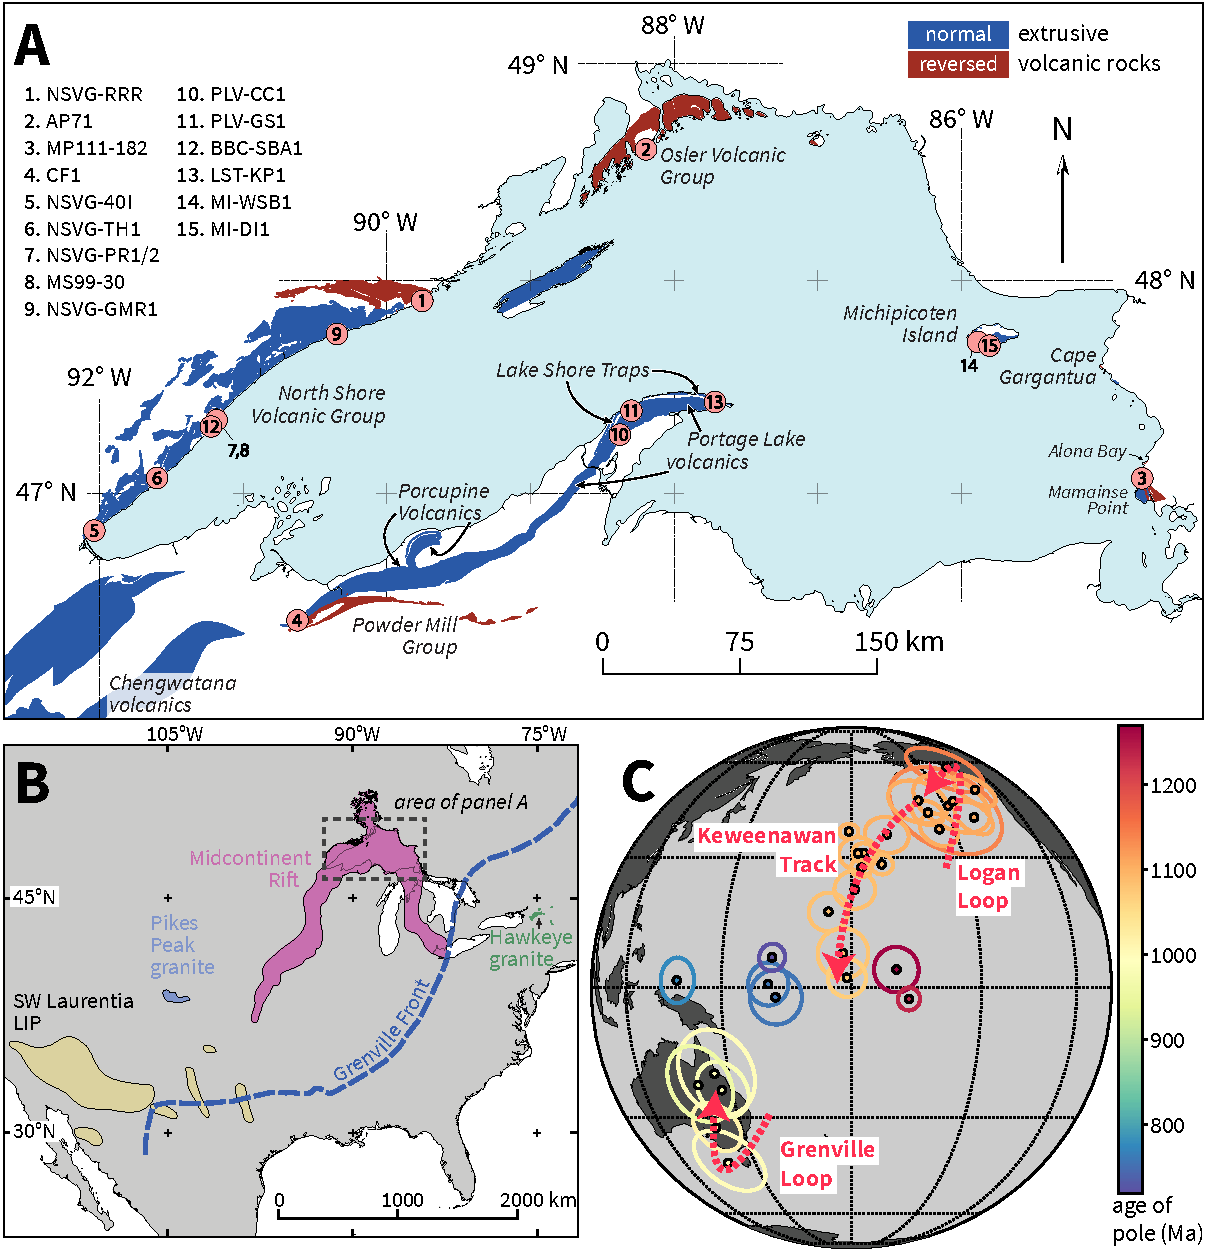
\includegraphics[width=6.5 in]{Figures/Fig1_MCR_map.pdf}
\caption{\small{\textbf{A: Geological map of Midcontinent Rift volcanics in the Lake Superior Region. The geomagnetic polarity is indicated by red (reversed) and blue (normal). Volcanic successions referred to in the text are labeled and the locations of geochronology samples are shown with circles and numbers that are keyed out to the sample name. B: Map of North America showing the position of the Midcontinent Rift inferred from surface geology and gravity anomaly data along with other ca. 1.1 Ga volcanic rocks including the SW Laurentia large igneous province (from \citealp{Bright2014a}) and the Hawkeye Granite (from \citealp{McLelland_ref}) as well as the the Grenville Front (from \citealp{Rivers2015a}) . C: Overview of Laurentia's apparent polar wander path from 1300 Ma to 700 Ma with the oldest pole coming from the Mackenzie large igneous province (ca. 1267 Ma) and the youngest from the Franklin large igneous province (ca. 720 Ma). The poles progress through the Logan Loop, the Keweenawan Track and the Grenville Loop.}}}
\label{fig:MCR_Map}
\end{figure}

The Midcontinent Rift system forms a $>$2500 km arcuate swath extending from the Lake Superior region, where rift rocks are exposed, far to the southwest into the Great Plains under Phanerozoic sedimentary cover where it is recognized by prominent gravity and aeromagnetic anomalies as well as drill core (Fig. \ref{fig:MCR_Map}; \citealp{Van-Schmus1985a, Van-Schmus1992a}). Geophysical anomalies related to the rift also extend to the southeast of Lake Superior under the Michigan Basin (Fig. \ref{fig:MCR_Map}; \citealp{Keller1983a}). While it is difficult to obtain precise U-Pb dates on the earliest mafic volcanics of the rift due to an overall lack of zircon, current constraints suggest that volcanism within the Midcontinent Rift initiated ca. 1110 Ma \citep{Davis1985a, Heaman2007a}. Older diabase dikes of the Abitibi swarm and coeval lamprophyre dikes in the northeastern Lake Superior region that were emplaced ca. 1140 Ma have been interpreted as magmatic precursors to rift development \citep{Queen1996a,Piispa2018a}. Volcanism within the Midcontinent Rift basin continued, albeit with hiatuses in different regions, until ca. 1083 Ma constrained by the youngest dated volcanics of the Michipicoten Island Formation (Figs. \ref{fig:geochron} and \ref{fig:chronostrat}; \citealp{Fairchild2017a}). The end of volcanic activity and active normal faulting occurred before the rift was able to completely dismember Laurentia. As a result, the rift is considered to have ``failed'' and geoscientists are left with a thick intact record of volcanism and sedimentation. Had the rift succeeded and led to the development of an ocean basin, North America would not exist as we know it today and there is a high likelihood that modification of the resulting margins by subsequent passive margin sedimentation and eventual collisional orogenesis would have resulted in a far less pristine record of rift-related rocks.

It has been estimated that more than 2 million km$^{3}$ of lava erupted throughout the history of volcanism in the Midcontinent Rift basin with more than 1.5 million km$^{3}$ of volcanics currently preserved \citep{Cannon1992b}. Thick portions of the succession are dominated by basaltic lava flows, many of which are interpreted to have been derived from an enriched mantle source rather than depleted mantle asthenosphere variably mixed with lithospheric mantle \citep{Shirey1997a}. Taken together, these features have been interpreted to indicate rifting above a plume-related thermal anomaly in the mantle \citep{Hutchinson1990a}. A more recent analogue for this type of tectonic setting is the early Cenozoic North Atlantic Igneous Province which is interpreted to have formed in a continental rift associated with a plume---although that event was associated with successful, rather than failed, continental rifting \citep{Hutchinson1990a, Saunders1997a}.

On the basis of chronostratigraphic interpretations of extrusive volcanics and the geochronology of intrusions, the Midcontinent Rift has been split by some researchers into four stages: an early stage (ca. 1109-1104 Ma), a latent stage (ca. 1104-1098 Ma), a main stage (ca. 1098-1090 Ma) and a late stage (ca. 1090-1083 Ma) \citep{Miller1996a, Davis1997a, Vervoort2007a}. The age ranges assigned to these stages are informed by both existing geochronology and are further refined by new U-Pb data presented in this paper. During the early stage, widespread flood basalt volcanism resulted in picritic to tholeiitic basalt flows across the Lake Superior region. The interpretation that there were low rates of eruption in portions of the Midcontinent Rift, such as the North Shore Volcanic Group, and a gap in the emplacement of shallow-level intrusions inferred from U-Pb dates \citep{Davis1997a, Vervoort2007a} led to the proposal of a latent stage which has also been referred to as the hiatus stage \citep{Miller2013a}. The continuation of volcanism during this interval in the eastern part of the present-day Lake Superior Basin, as recorded at Mamainse Point, may explain why additional geomagnetic reversals are seen through the stratigraphy there prior to a regional volcanic hiatus and deposition of a thick conglomerate \citep{Swanson-Hysell2014a}. The main stage of rift volcanism resulted in the outpouring of thick successions of tholeiitic basalts that are exposed within the North Shore Volcanic Group \citep{Green1989a}, the Portage Lake Volcanics \citep{Nicholson1997a} and the upper portion of the succession at Mamainse Point \citep{Shirey1994a}. Much of the thickness of the $>$20 km of lava flows that have been revealed through seismic profiles to underlie the center of Lake Superior (the GLIMPCE lines; \citealp{Cannon1992b}) are interpreted to have erupted during this stage of rift development.

Volcanism that persisted following this interval of particularly voluminous eruptions is referred to as the late stage. These late stage lava flows include the volcanics within the Copper Harbor Conglomerate known as the Lake Shore Traps \citep{Lane1911a, Davis1990a} and the youngest volcanics exposed on Michipicoten Island \citep{Annells1974a, Fairchild2017a}. The Davieaux Island Rhyolite of the Michipicoten Island Formation at 1083.52 $\pm$ 0.23 (2$\sigma$ internal error) is the youngest igneous rock that has been dated from the Midcontinent Rift (Figs. \ref{fig:geochron} and \ref{fig:chronostrat}; \citealp{Fairchild2017a}). While sedimentary rocks are found as interflow deposits throughout many successions of rift volcanics, it is during and after this late stage of volcanic activity that sedimentary rocks become dominant with the deposition of the Oronto Group. The Copper Harbor Conglomerate is a formation of the Oronto Group that interfingers with lavas of the Lake Shore Traps. Above the Copper Harbor Conglomerate is the Nonesuch Formation and then the Freda Formation. Taken together, these Oronto Group sedimentary rocks are more than 5500 meters thick. The accommodation space for this deposition came from post-rift thermal subsidence associated with conductively cooling mantle throughout the region where the lithosphere had been dramatically thinned \citep{Cannon1992b}.

Overall, the protracted history of volcanism, the prodigious volume, and the lack of metamorphism (beyond what occurred during rift-related burial) are what make the volcanics, intrusives and rift-related sediments of the Keweenawan Rift excellent archives of paleogeographic information.

\section{GEOMAGNETIC POLARITY}

To aid in the discussion of geomagnetic polarity zones, we propose naming them following the guidelines of the International Commission on Stratigraphy. To date, four polarity zones have been recognized within the Midcontinent Rift (Figs. \ref{fig:geochron} and \ref{fig:chronostrat}).

\begin{figure}
\centering
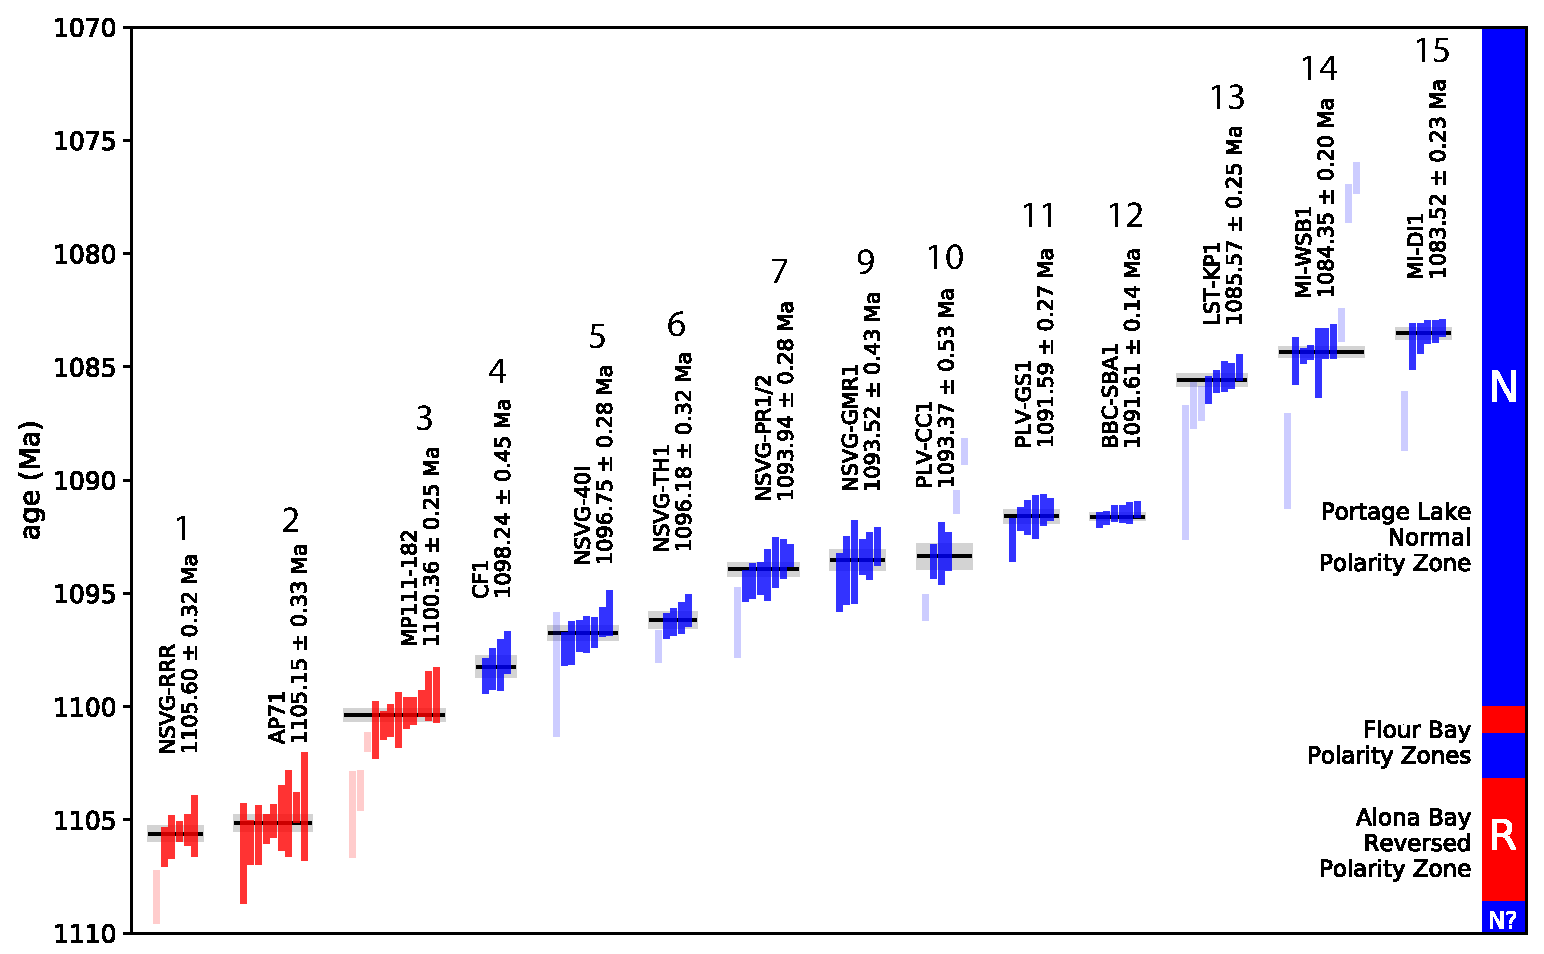
\includegraphics[width=6.5 in]{Figures/Fig2_MCR_dates.pdf}
\caption{\small{\textbf{Date distribution plots for CA-ID-TIMS $^{206}$Pb/$^{238}$U dates from the Midcontinent Rift colored by magnetic polarity (red for reversed, blue for normal). Vertical bars represent 2$\sigma$ analytical uncertainty of individual zircon analyses; darker bars are data used in age calculations while light bars were excluded based on interpreted inheritance or Pb-loss. Horizontal lines and shaded bands signify weighted mean dates and their 2$\sigma$ uncertainties. All dates are from this study with the exception of MP111-182 which was published in \cite{Swanson-Hysell2014a} and BBC-SBA1/MI-WSB1/MI-DI1 which were published in \cite{Fairchild2017a}. See Table S1 in Data Repository Item for complete U-Pb data, as well as the text and Table 1 for details regarding the geochronology. The interpreted geomagnetic polarity timescale is shown to the right. The geomagnetic reversal associated with the end of the Alona Bay reversed-polarity zone and the normal to reversed reversal within the Flour Bay polarity zones are constrained to have occurred between 1105.15 $\pm$ 0.33 Ma and 1100.36 $\pm$ 0.25 Ma. The geomagnetic reversal associated with the start of the Portage Lake normal-polarity zone is constrained to have occurred between 1100.36 $\pm$ 0.25 Ma and 1098.24 $\pm$ 0.45 Ma.}}}
\label{fig:geochron}
\end{figure}

\begin{itemize}
\item \textbf{Alona Bay reversed-polarity zone}: The first directions of reversed polarity published from Midcontinent Rift lavas were from the lavas exposed at Alona Bay which is 13 km north of Mamainse Point in eastern Lake Superior (Fig. \ref{fig:MCR_Map}; \citealp{Dubois1962a}). These lavas are nearby, and correspond to, the lower reversed polarity zone in the Mamainse Point stratigraphy \citep{Palmer1970a}. This polarity zone was referred to as ``lower reversed" in \cite{Swanson-Hysell2009a,Swanson-Hysell2014a}. The Alona Bay reversed-polarity zone is associated with the early stage of Midcontinent Rift magmatic activity. On the basis of the geomagnetic polarity implications of dual-polarity data from the Umkondo large igneous province of the Kalahari Craton, \cite{Swanson-Hysell2015b} suggested via correlation that this polarity zone started at ca. 1109 Ma. Reversed polarity continued until after 1105.15 $\pm$ 0.33 Ma based on geochronology from the Osler Volcanic Group (Figs. \ref{fig:geochron} and \ref{fig:Osler_Map}).
\item \textbf{Flour Bay normal-polarity zone} and \textbf{Flour Bay reversed-polarity zone}: The only extrusive succession where paleomagnetic data have definitively been developed from the normal and reversed polarity zones between the older Alona Bay reversed-polarity zone and the Portage Lake normal-polarity zone (defined below) are the volcanics in the vicinity of Flour Bay in the Mamainse Point lavas \citep{Palmer1970a,Robertson1973a,Swanson-Hysell2009a}. Therefore, we propose naming both the normal and reversed polarity zone after Flour Bay. These polarity zones were referred to as ``lower normal'' and ``upper reversed'' in \cite{Swanson-Hysell2009a,Swanson-Hysell2014a}. The Flour Bay reversed-polarity zone was ongoing at 1100.36 $\pm$ 0.25 Ma (Fig. \ref{fig:geochron}; \citealp{Swanson-Hysell2014a}). Normally magnetized intrusive rocks from the Coldwell Complex \citep{Kulakov2014a} may correspond to the Flour Bay normal-polarity zone although they could potentially be from the normal polarity zone that preceded the Alona Bay reversed-polarity zone. These polarity zones are associated with what has been interpreted as the latent stage of Midcontinent Rift magmatic activity \citep{Swanson-Hysell2014a}.
\item \textbf{Portage Lake normal-polarity zone}: \cite{Dubois1955a} was the first to measure paleomagnetic directions from Keweenawan volcanics and sedimentary rocks and found WNW and downward directions for samples of Portage Lake Volcanics, Lake Shore Trap volcanics and Copper Harbor Conglomerate sandstones. We therefore propose that this polarity zone should be referred to as the Portage Lake normal-polarity zone in recognition of where it was first identified within the Portage Lake Volcanics near Portage Lake in the Keweenaw Peninsula of Michigan. This polarity zone --- referred to as ``upper normal'' in \cite{Swanson-Hysell2009a,Swanson-Hysell2014a} --- is associated with both the main and late stages of Midcontinent Rift magmatic activity. \cite{Driscoll2016a} suggest that the Portage Lake normal-polarity zone is a geomagnetic superchron with a duration on the order of 40 million years, which they term the Keweenawan Normal Superchron. Geochronology from this study show that the polarity zone likely started prior to 1098.24 $\pm$ 0.45 Ma, was certainly ongoing by 1096.75 $\pm$ 0.28 Ma, and continued past 1083.52 $\pm$ 0.23 Ma (Fig. \ref{fig:geochron}).
\end{itemize}

\section{METHODS}

\subsection{Paleomagnetic data compilation}

Abundant paleomagnetic data have been generated from extrusive lava flows and intrusive igneous units throughout the Midcontinent Rift. This contribution is focused on the calculation of paleomagnetic poles from data developed from lava flows for two principal reasons:
\begin{enumerate}
\item Interflow sediments and lava flow tops provide a means to estimate paleohorizontal that is more robust than what is possible for intrusive rocks. Rocks across the Lake Superior Region generally tilt towards the axis of the rift. While the tilt of intrusions can sometimes be estimated using data from nearby flows, it can be directly measured in extrusive successions. As a result, the tilt-corrected directions used to estimate pole position can be considered more reliable from lavas than from intrusions.
\item The development of a paleomagnetic pole requires paleomagnetic directions from many individual sites wherein each site can be considered to record a distinct snapshot of the geomagnetic field. If a volcanic unit within a sequence of flows has been dated, it is more straightforward to associate a sequence of lava flows with that date than in the case of intrusions. If an intrusion is dated, it is sometimes unclear what other intrusions in the vicinity should be associated with the dated unit and which may be substantially older or younger. The large magnitude of apparent polar wander ongoing at this time results in this issue being more problematic in the Midcontinent Rift than many other igneous provinces.
\end{enumerate}

Paleomagnetic poles and their associated 95$\%$ cones of confidence (A$_{95}$) from Midcontinent Rift rocks have been determined in different ways in different studies given the range of time over which they have been developed. This study uses the methodology as summarized by \cite{Butler1992a} and strongly advocated for by \citet{Deenen2011a}. First, a site-mean virtual geomagnetic pole (VGP) is calculated from each site-mean direction whereby a site is defined as a single igneous cooling unit. Subsequently, a paleomagnetic pole is calculated using Fisher statistics treating each VGP as a point on a unit sphere to yield a mean pole and associated A$_{95}$ confidence cone. The rational for this treatment of the data, rather than transforming the directional mean and its confidence ellipse into pole space, is that the most significant source of scatter in a data set of site mean directions is interpreted to be that from paleosecular variation of the geomagnetic field \citep{Deenen2011a}. The leading statistical models of geomagnetic secular variation, developed to fit modern and geologically recent data, are constructed such that time variation of the field results from changing spherical harmonic coefficients drawn from Gaussian distributions---termed a ``giant Gaussian process'' \cite[e.g.,][]{Constable1988a, Tauxe2004a}. An aspect of these paleosecular variation models is that the predicted distributions of VGPs are circularly symmetric. This circular symmetry of poles on the globe does not result in a circularly symmetric distribution of paleomagnetic directions in geologic materials that record the geomagnetic field. Therefore, calculating the Fisher statistics for VGPs is preferable to transforming the circularly symmetric $\alpha_{95}$ directional error ellipse into pole space and reporting the major and minor axis (\textit{dp} and \textit{dm}) of the resulting ellipse.

In contrast, within an individual lava flow all samples should record the same spot reading of the geomagnetic field and therefore any deviation from this mean direction can be considered to be a result of random sampling and measurement errors. Therefore, it is appropriate to apply Fisher statistics to the distribution of declination/inclination unit vectors in directional space in order to calculate the site mean and the 95$\%$ cone of confidence ($\alpha_{95}$). This approach is taken in this study  on paleomagnetic data from the literature as well as new data. Previously published data were compiled into Magnetics Information Consortium (MagIC) format at the site level and contributed to the MagIC database.

\subsection{Paleomagnetic data development}

Demagnetization and measurements associated with new paleomagnetic data presented in this study were conducted in the UC Berkeley Paleomagnetism Lab using a 2G Enterprises DC-SQUID superconducting rock magnetometer equipped with an automated pick-and-place sample changer system and an inline coils capable of preforming alternating field demagnetization. The magnetometer is housed in a magnetostatic shield with magnetic fields $<$500 nT. A quartz glass sample rod brings the samples into the measurement region and is typically measured at 5 x 10$^{-12}$ Am$^2$. Samples being analyzed via thermal demagnetization, samples first underwent liquid nitrogen immersion following the measurement of natural remanent magnetization (NRM). During this liquid nitrogen step, the samples were equilibrated at 77 K and then warmed back to room temperature all in a low-field environment ($<$10 nT). This step was implemented with the goal of preferentially removing remanence associated with multidomain magnetite. Such multidomain grains undergo low-temperature demagnetization when cycled through the isotropic point ($\sim$130 K) and the Verwey transition ($\sim$120 K; \citealp{Verwey1939a, Feinberg2015a}). Following acquisition of the data, principal component analysis \citep{Kirschvink1980a} was conducted using the PmagPy software package (\url{https://github.com/PmagPy}; \citealp{Tauxe2016a}). All new and compiled data associated with this work are available within a Github repository associated with this article (\url{https://github.com/Swanson-Hysell-Group/2018_Midcontinent_Rift}) and the MagIC database (\url{https://www.earthref.org/MagIC/doi/10.1130/B31944.1}).

\subsection{U-Pb geochronology}

New high-resolution age constraints on paleomagnetic poles are achieved through U-Pb zircon geochronology carried out at the MIT Isotope Lab using chemical abrasion isotope-dilution thermal ionization mass spectrometry (CA-ID-TIMS). Zircon crystals were isolated from bulk rock by standard crushing and pulverizing followed by magnetic and high-density liquid separation techniques. All U-Pb analyses were made on single zircon crystals that were pre-treated by a chemical abrasion technique modified after \cite{Mattinson2005a} and analyzed following the procedures described in \cite{Ramezani2011a}. Chemical abrasion was achieved through leaching of zircon in 29 M hydrofluoric acid at 210\textdegree C for $\sim$12 hours. This intensive leach schedule often resulted in extensive disintegration or near complete dissolution of zircon crystals, but was deemed necessary in order to fully mitigate the effects of Pb loss due to accumulated radiation damage in the zircon crystals.

The EARTHTIME ET535 mixed $^{205}$Pb€“-$^{233}$U€“-$^{235}$U isotopic tracer and, when appropriate, the ET2535 tracer solution containing additional $^{202}$Pb \citep{Condon2015a, McLean2015a} were used to spike the pre-treated zircons prior to complete dissolution and analysis. A VG Sector 54 or an Isotopx X62 multi-collector thermal ionization mass spectrometer equipped with Daly photomultiplier ion-counting systems was used to measure Pb and U isotopic ratios. Data reduction, U-Pb date calculation and error propagation were carried out with Tripoli and ET$\_$Redux algorithms and software \citep{Bowring2011a, McLean2011a}.

Sample dates representing zircon crystallization ages are calculated based on the weighted mean $^{206}$Pb/$^{238}$U date of the analyzed zircons from each sample. For some samples, older zircon analyses interpreted as xenocrysts or antecrysts were excluded from the weighted mean. Weighted mean date uncertainties are given in the $\pm$ \textit{X/Y/Z} format, where \textit{X} is the 2$\sigma$ analytical error exclusive of external sources of uncertainty, \textit{Y} includes \textit{X} and additional tracer calibration error, and \textit{Z} incorporates the U decay constant uncertainties of \cite{Jaffey1971a}. The uncertainty from tracer calibration (\textit{Y}) must be taken into account when comparisons are made between U-Pb dates from different techniques or from different ID-TIMS labs that utilize different tracers. For comparison between dates from different chronometers (e.g., U-Pb versus $^{40}$Ar-$^{39}$Ar or Re-Os), the total uncertainty (\textit{Z}) must be considered. The U-Pb geochronology presented here can be integrated with that reported in \cite{Swanson-Hysell2014a} and \cite{Fairchild2017a} at the \textit{X} uncertainty level without taking into account \textit{Y} or \textit{Z} given the use of the same tracer and analytical protocols. Calculated weighted mean dates and their uncertainties are summarized in Table \ref{tab:geochron} and illustrated with date distribution plots in Figure \ref{fig:geochron}.

There are important considerations to make when comparing recent high-precision CA-ID-TIMS U-Pb geochronology (\citealp{Swanson-Hysell2014a}; \citealp{Fairchild2017a}; this paper) to previously published U-Pb geochronology from the Midcontinent Rift and elsewhere. The first consideration is that many existing analyses in the literature were developed prior to the advent of higher precision techniques that enable isotopic analyses to be conducted on single zircon crystals. Data were instead developed from multiple grains in a single analysis which can potentially result in a skew toward older ages due to unrecognized xenocrystic zircons. In contrast, single-zircon analyses at high precision facilitate the identification of such outliers in addition to the detection of open-system behavior due to radiation-induced Pb-loss. Another important consideration is that while most published U-Pb ages from the Midcontinent Rift have been calculated as $^{207}$Pb/$^{206}$Pb dates from discordant zircon analyses, this study is focused on the development of high-precision $^{206}$Pb/$^{238}$U dates from chemically-abraded zircon. The chemical abrasion technique of \cite{Mattinson2005a} has proven more effective than prior mechanical abrasion methods \citep{Krogh1982a} leading to improved accuracy in U-Pb zircon geochronology by the ID-TIMS method. While mechanical abrasion was beneficial, it is less effective in eliminating Pb-loss leading to discordant analyses and a reliance on $^{207}$Pb/$^{206}$Pb or upper concordia intercept dates. Effective elimination of Pb-loss through chemical abrasion allows the more robust, but sensitive to Pb-loss, $^{206}$Pb/$^{238}$U chronometer to be exploited in producing more reliable dates. $^{206}$Pb/$^{238}$U dates are more precise given that the error contribution from common lead correction is systematically smaller than for $^{207}$Pb/$^{235}$U and $^{207}$Pb/$^{206}$Pb dates. $^{206}$Pb/$^{238}$U dates are also considered more accurate because of suspected inaccuracies in the decay constant of $^{235}$U \citep{Schoene2006a, Mattinson2010a} that result in typically older $^{207}$Pb/$^{235}$U (and thus older $^{207}$Pb/$^{206}$Pb and concordia intercept) dates. Another difference comes from the progress that has been made in constraining the present-day isotopic ratio of natural uranium which needs to be assumed in U-Pb analysis by the ID-TIMS method. The value for the $^{238}$U/$^{235}$U ratio is now taken to be 137.818 $\pm$ 0.044 (2$\sigma$) rather than 137.88 \citep{Hiess2012a} and this updated ratio is used in the reduction of U-Pb isotopic data in this study (as well as in \citealp{Swanson-Hysell2014a} and \citealp{Fairchild2017a}). For rocks that are ca. 1 Ga, $^{207}$Pb/$^{206}$Pb dates calculated using this ratio are roughly 1 million years younger than if they were calculated using the outdated ratio \citep{Hiess2012a}. Consequently, systematic biases between the majority of previously published U-Pb geochronology from the Midcontinent Rift and more recent CA-TIMS geochronology from the same units are to be expected. Our analysis of rates is focused on comparisons between $^{206}$Pb/$^{238}$U dates to minimize these complications and be able to compare dates at the level of analytical uncertainty ($\pm$ \textit{X}).

\begin{table}[h!]
\footnotesize
\caption{Summary of CA-ID-TIMS $^{206}$Pb/$^{238}$U dates from Midcontinent Rift volcanics}
\begin{tabular}{|p{2.2 cm}|p{2 cm}|p{1.6 cm}|c|ccc|c|c|p{1.7 cm}|}
\hline
Sample & Group & Latitude & $^{206}$Pb/$^{238}$U & \multicolumn{3}{|c|}{Error (2$\sigma$)} & MSWD & n & Reference \\
 &  & Longitude & date (Ma) & X & Y & Z & & & \\
\hline
NSVG-RRR \textit{Red Rock Rhyolite} & North Shore Volcanic Group (lower NE sequence) & 47.90402\textdegree N 89.75767\textdegree W & 1105.60 & 0.32 & 0.42 & 1.3 & 0.64 & 5 & this study \\
\hline
AP71 \newline \textit{Agate Point rhyolite flow} & Osler Volcanic Group & 48.60716\textdegree N 88.19866\textdegree W & 1105.15 & 0.33 & 0.56 & 1.3 & 1.4 & 9 & this study\\
\hline
MP111-182 \newline \textit{Flour Bay tuff} \newline & Mamainse Point Formation & 47.0691\textdegree N  84.7427\textdegree W & 1100.36 & 0.25 & 0.42 & 1.2 & 1.4 & 9 & \cite{Swanson-Hysell2014a} \\
\hline
CF1 \textit{Sheep Farm Rhyolite} & Kallander Creek Volcanics & 46.37547\textdegree N 90.63715\textdegree W & 1098.24 & 0.45 & 0.63 & 1.3 & 1.3 & 4 & this study \\
\hline
NSVG-40I \textit{40th Avenue Icelandite} & North Shore Volcanic Group (upper SW sequence) & 46.82037\textdegree N 92.04131\textdegree W & 1096.75 & 0.28 & 0.53 & 1.3 & 1.7 & 7 & this study \\
\hline
NSVG-TH1 \textit{icelandite within Two Harbors basalts} & North Shore Volcanic Group (upper SW sequence) & 47.0703\textdegree N 91.6039\textdegree W & 1096.18 & 0.32 & 0.54 & 1.3 & 0.83 & 4 & this study \\
\hline
NSVG-PR1$\&$PR2 \textit{Palisade Rhyolite} & North Shore Volcanic Group (upper SW sequence) & 47.34445\textdegree N 91.18944\textdegree W & 1093.94 & 0.28 & 0.52 & 1.3 & 2.6 & 7 & this study \\
\hline
MS99-30 \newline\textit{Palisade Rhyolite} & North Shore Volcanic Group (upper SW sequence) & 47.346\textdegree N 91.188\textdegree W & 1094.2 & 0.2 & 0.4 & 1.5 & 0.7 & 19 & \cite{Schoene2006a} \\
\hline
NSVG-GMR1 \textit{Grand Marais Rhyolite} & North Shore Volcanic Group (upper NE sequence) & 47.74943\textdegree N 90.35150\textdegree W & 1093.52 & 0.43 & 0.57 & 1.3 & 1.0 & 6 & this study \\
\hline
PLV-CC1 \newline\textit{Copper City Flow} & Portage Lake Volcanics & 47.2758\textdegree N 88.3803\textdegree W & 1093.37 & 0.53 & 0.69 & 1.4 & 0.33 & 3 & this study \\
\hline
PLV-GS1 \textit{Greenstone Flow} & Portage Lake Volcanics & 47.3882\textdegree N 88.3005\textdegree W & 1091.59 & 0.27 & 0.52 & 1.3 & 1.4 & 6 & this study \\
\hline
BBC-SBA1 \newline\textit{Silver Bay aplite intrusion} & Beaver Bay Complex & 47.3143\textdegree N 91.2281\textdegree W & 1091.61 & 0.14 & 0.30 & 1.2 & 1.0 & 6 & this study \\
\hline
LST-KP1 \newline\textit{Keweenaw Point andesite} & Lake Shore Traps & 47.4331\textdegree N 87.7147\textdegree W & 1085.57 & 0.25 & 0.50 & 1.3 & 1.5 & 5 & \cite{Fairchild2017a} \\
\hline
MI-WSB1 \textit{West Sand Bay tuff} & Michipicoten Island Formation & 47.7117\textdegree N 85.8871\textdegree W & 1084.35 & 0.20 & 0.34 & 1.2 & 0.88 & 6 & \cite{Fairchild2017a} \\
\hline
MI-DI1 \textit{Davieaux Island Rhyolite} & Michipicoten Island Formation & 47.6947\textdegree N 85.8056\textdegree W & 1083.52 & 0.23 & 0.35 & 1.2 & 0.86 & 5 & \cite{Fairchild2017a} \\
\hline
\end{tabular}
\begin{tablenotes}[para,flushleft]
Notes: X--internal (analytical) uncertainty in the absence of all external or systematic errors; Y--uncertainty incorporating the U-Pb tracer calibration error; Z--uncertainty including X and Y, as well as the uranium decay constant uncertainty; MSWD--mean square of weighted deviates; n--number of zircon analyses included in the calculated date.
\end{tablenotes}
\label{tab:geochron}
\end{table}

\section{Volcanic Successions}

\begin{figure}
\centering
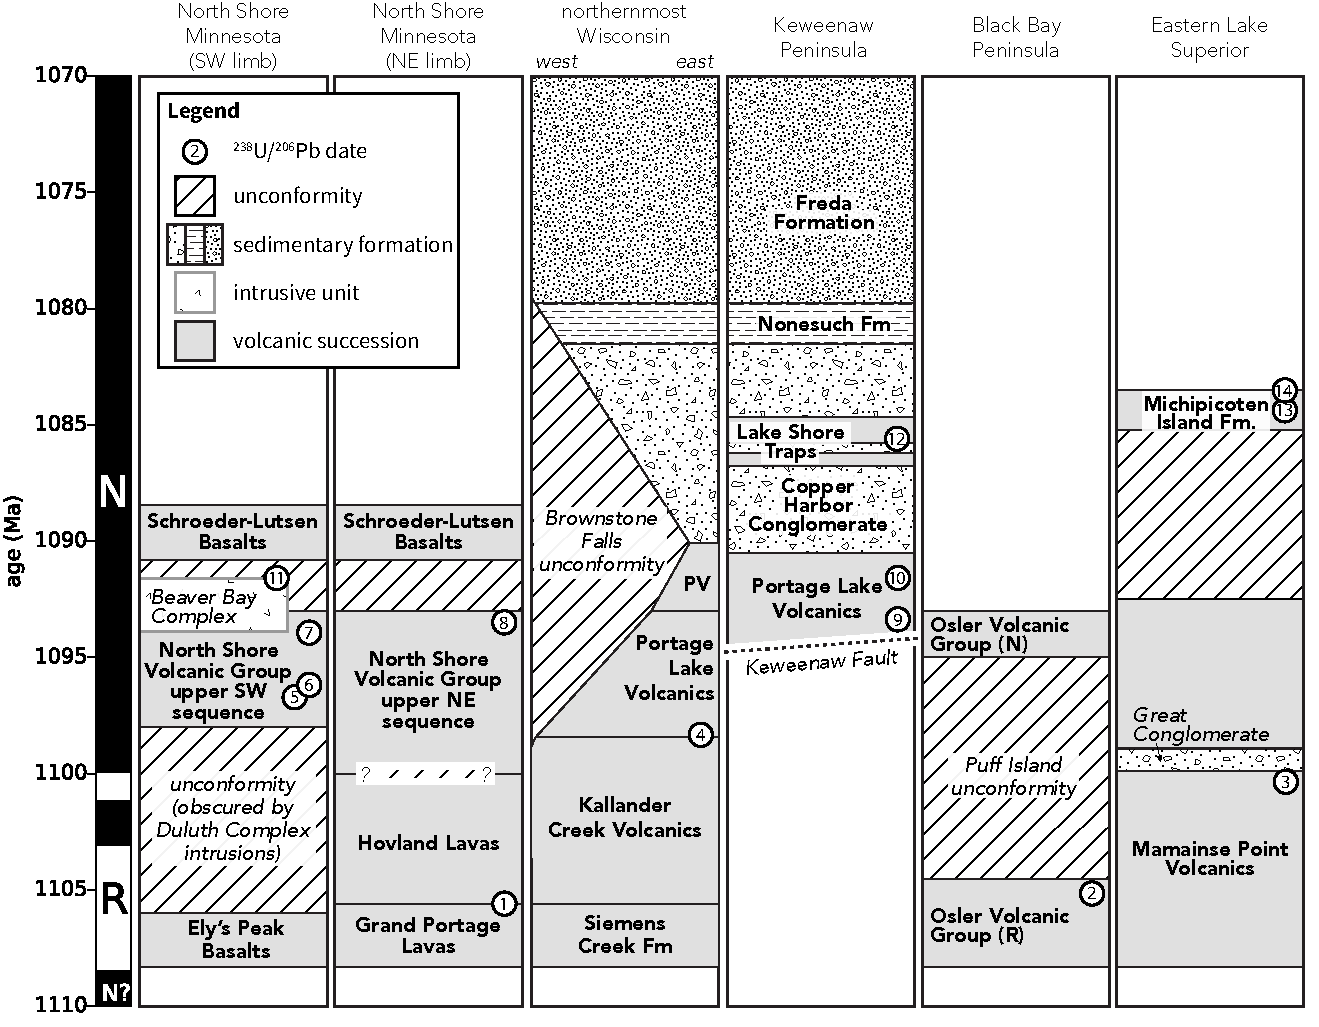
\includegraphics[width=6.5 in]{Figures/Fig3_MCR_chronostrat.pdf}
\caption{\small{\textbf{Chronostratigraphic correlation of Midcontinent Rift volcanic sequences informed by new U-Pb dates. The numbered circles correspond to CA-ID-TIMS $^{206}$Pb/$^{238}$U dates using the same numbering scheme as in Figures \ref{fig:MCR_Map} and \ref{fig:geochron}. The analytical uncertainty, which should be used when comparing these dates to one another, is less than the time represented by the height of the circles. Extrapolated eruption rates, paleomagnetic data (both polarity and pole position) and $^{207}$Pb/$^{206}$Pb dates (not shown) inform the chronostratigraphic interpretation, but the chronostratigraphy is most robust in the proximity of the $^{206}$Pb/$^{238}$U dates. PV: Porcupine Volcanics; Fm: Formation.}}}
\label{fig:chronostrat}
\end{figure}

\subsection{Osler Volcanic Group}

\subsubsection{Background and Paleomagnetism}

The Osler Volcanic Group is a sequence of Midcontinent Rift lava flows exposed on Black Bay Peninsula and throughout the Lake Superior Archipelago in northern Lake Superior (Fig. \ref{fig:Osler_Map}). The stratigraphically lowest lavas are primitive Mg-rich tholeiites that continue up into lower-Mg tholeiites \citep{Keays2015a}. \cite{Halls1974a} conducted the first paleomagnetic study of these flows targeting the upper portion of the succession in order to test for the presence of a geomagnetic polarity reversal that had been interpreted from aeromagnetic data \citep{Halls1972a}. That work determined that the Osler Volcanic Group flows were of dominantly reversed polarity with a paleomagnetic reversal near the top of the exposed stratigraphy. This reversal is associated with an angular unconformity of $\sim$20\textdegree$\;$that is exposed on Puff Island (Fig. \ref{fig:Osler_Map}). The unconformity is associated with the deposition of the Puff Island conglomerate which is dominated by basalt clasts and also contains clasts of felsic porphry. While the sole exposure of the unconformity is on Puff Island and the overlying normally magnetized volcanics are only exposed on Puff Island and a few small islands in the immediate vicinity (Fig. \ref{fig:Osler_Map}), aeromagnetic data suggest that the unconformity extends along the entire $>$100 km length of the Lake Superior Archipelago \citep{Halls1972a, Halls1974a}. The angular nature of this unconformity and its association with a geomagnetic reversal suggest that it corresponds to a significant temporal gap in the record of volcanism within the Osler Volcanic Group (Fig. \ref{fig:chronostrat}). The unconformity may be associated with rift flank uplift that occurred during extension that confined lavas to a narrower region of the central graben. Such rift flank uplift would have been followed by broader thermal subsidence, at which time lava flows again covered the region.

\begin{figure}[!h]
\centering
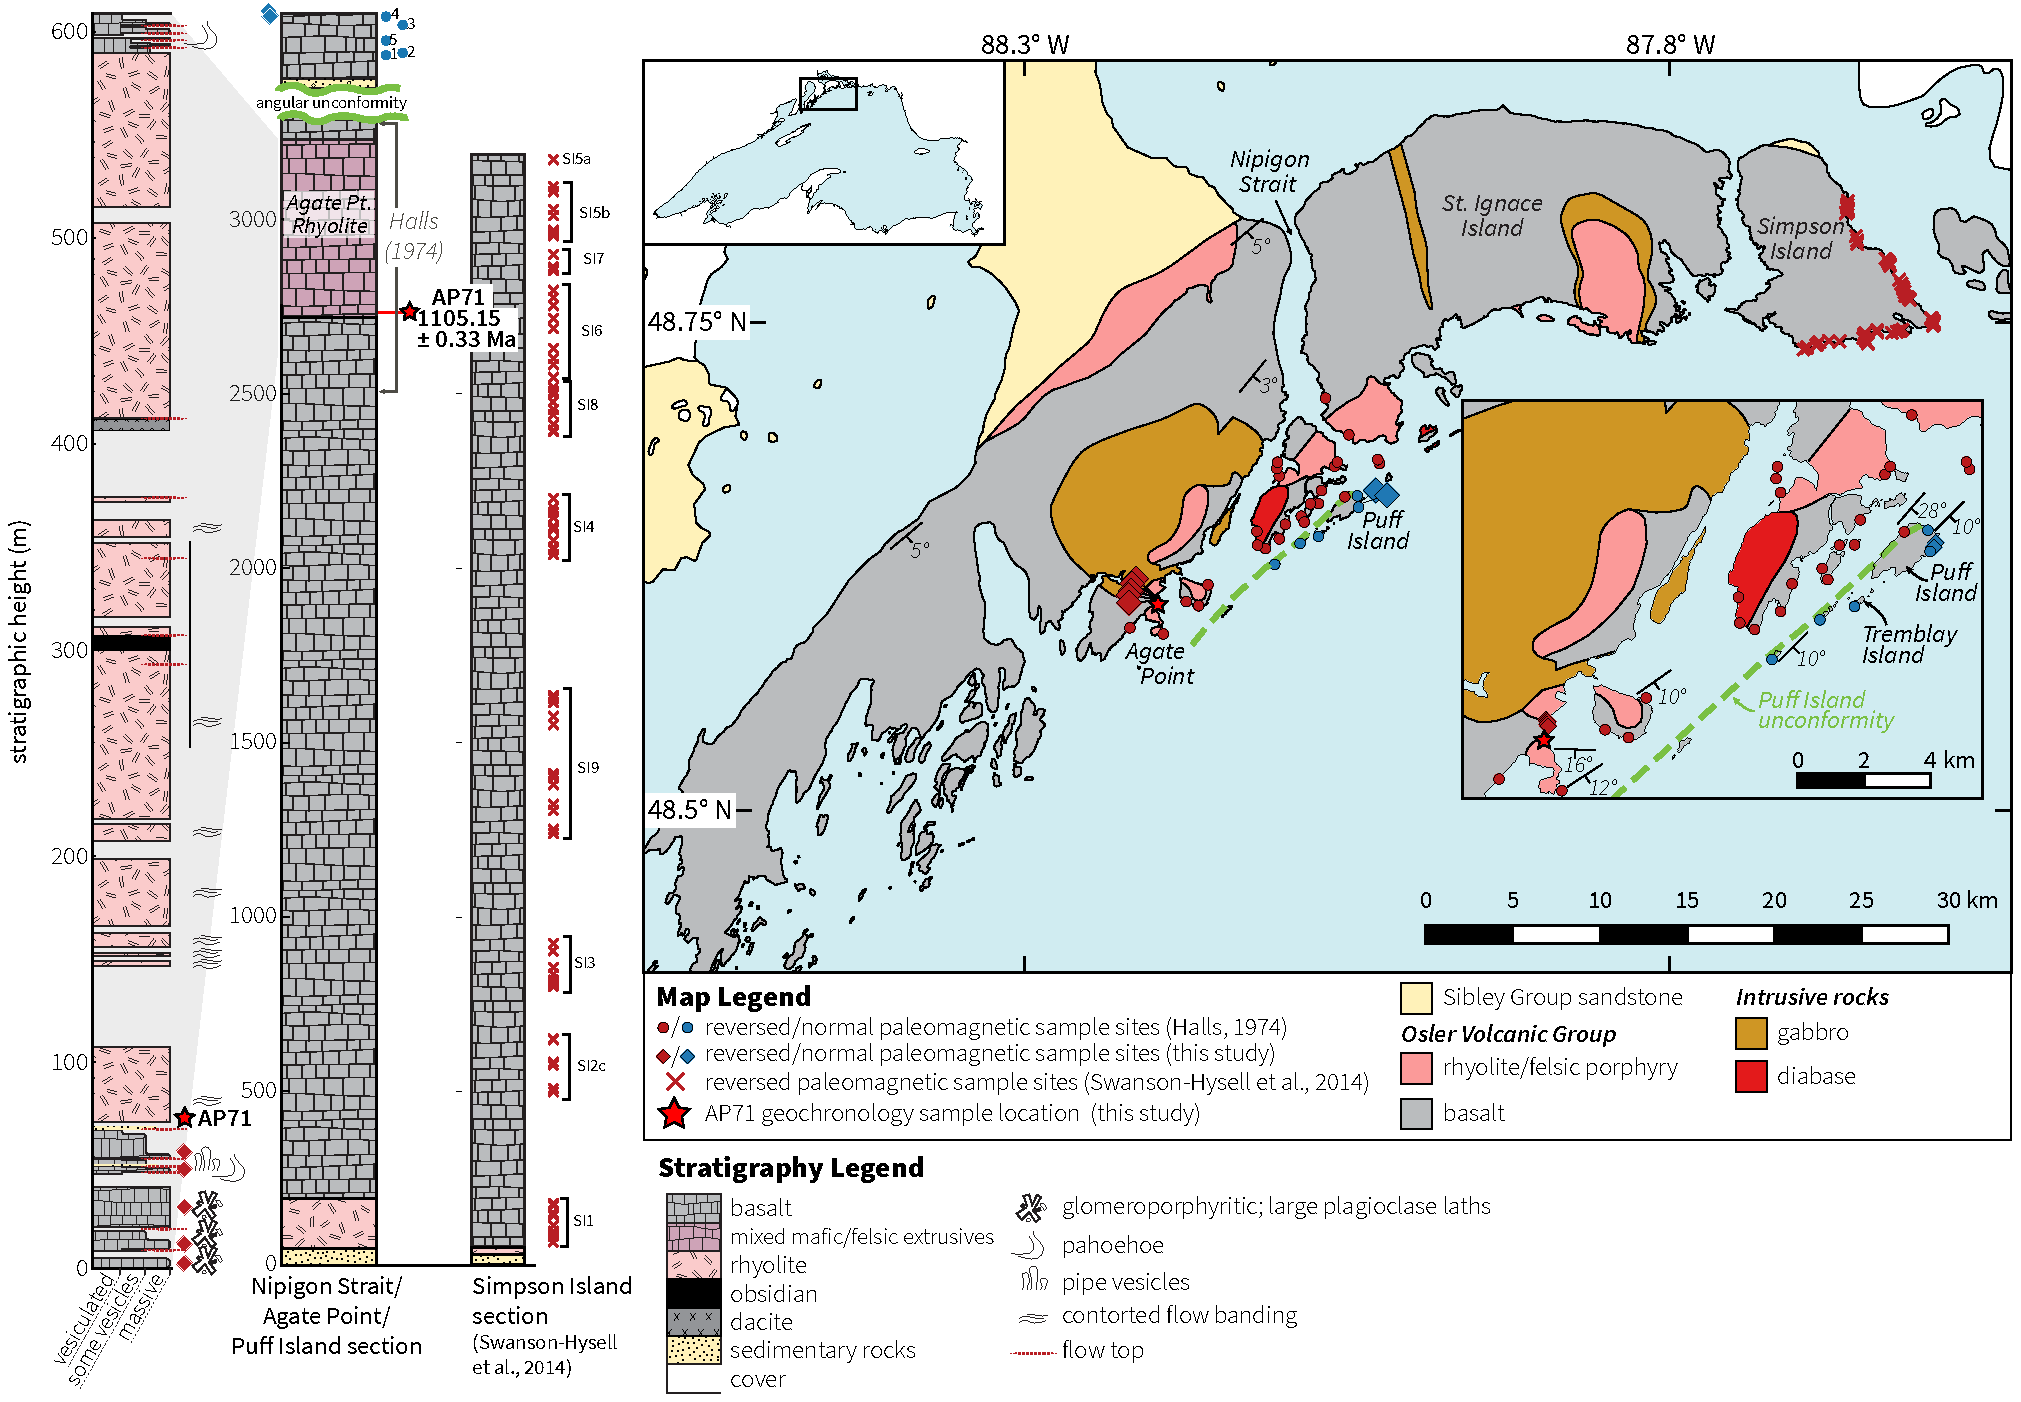
\includegraphics[width=6.5 in]{Figures/Fig4_Osler_map.pdf}
\caption{\small{\textbf{Geological map and summary Midcontinent Rift stratigraphy of the Lake Superior Archipelago, Ontario, Canada. Composite stratigraphic columns with the position of paleomagnetic sites from \cite{Halls1974a}, \cite{Swanson-Hysell2014b} and this study are shown for the Nipigon Strait/Agate Point/Puff Island region and for Simpson Island. The \cite{Halls1974a} sites are in the upper portion of the stratigraphy as indicated with the red bracket. Exposures of extrusive rhyolitic lava flows occur on Agate Point with basaltic lavas below and above. The more detailed stratigraphic section for Agate Point shows the position of the dated rhyolite (AP71). The geological map is modified from \cite{Carter1973a}. The map, and the zoomed-in inset, show the position of the Puff Island unconformity and sample sites.}}}
\label{fig:Osler_Map}
\end{figure}

The paleomagnetic data presented in \cite{Halls1974a} from the reversed polarity lavas were from flows near the top of that polarity interval such that they are stratigraphically within 800 meters of the overlying angular unconformity (Fig. \ref{fig:Osler_Map}). \cite{Swanson-Hysell2014b} conducted a paleomagnetic study that spanned the Osler Volcanic Group flows from their base atop the underlying Sibley Group up to the upper portions of the exposed reversed polarity flows (Fig \ref{fig:Osler_Map}). This work showed that the Osler Volcanic Group flows have simple, generally single-component remanence upon demagnetization that is dominantly held by (titano)magnetite. The analysis of the site means in the study determined that there was a significant change in direction between the flows in the lower third of the reversed polarity stratigraphy and those in the upper third of the stratigraphy. This change in pole position was interpreted as progression along the APW path due to equatorward motion of Laurentia as is also recorded in the lower polarity zone at Mamainse Point. In the current compilation, we include the lower Osler reversed pole (218.6\textdegree E, 40.9\textdegree N, A95: 4.8\textdegree, N: 30; Fig. \ref{fig:VGP}; Table \ref{tab:poles}) developed with data from \cite{Swanson-Hysell2014b} and an upper Osler reversed pole (203.4\textdegree E, 42.3\textdegree N, A95: 3.7\textdegree, N: 64; Fig. \ref{fig:VGP}; Table \ref{tab:poles}) with data from \cite{Halls1974a}, \cite{Swanson-Hysell2014b} and new thermal demagnetization data from five additional basalt flows (AP1-AP5; Table \ref{tab:pmag_sites}; Fig. \ref{fig:Osler_Map}). These new paleomagnetic sites were collected from the exposure at Agate Point in the immediate vicinity of the rhyolite dated in this study that is described in more detail below (Fig. \ref{fig:Osler_Map}). Both the lower and upper Osler reversed poles are from the Alona Bay reversed-polarity zone.

\begin{table}[h!]
\footnotesize
\caption{Summary of new site level paleomagnetic data utilized for paleomagnetic poles}
\begin{tabular}{|l|l|l|r|r|r|r|r|r|r|r|}
\hline
volcanic succession & site name & n & dec & inc & k & R & $\alpha_{95}$ & VGP lat & VGP lon \\
\hline
Osler Volc. Group (Agate Point) & AP1 &  8 &  102.9 & -73.3 &  535 &  7.9869 &  2.4 & -46.0 &  45.6 \\
Osler Volc. Group (Agate Point) & AP2 &  8 &  94.4 & -64.7 &  562 &  7.9875 &  2.3 & -35.4 &  34.6 \\
Osler Volc. Group (Agate Point) & AP3 &  8 &  105.4 & -59.0 &  358 &  7.9804 &  2.9 & -37.9 &  21.8 \\
Osler Volc. Group (Agate Point) & AP4 &  8 &  89.5 & -69.1 &  177 &  7.9603 &  4.2 & -36.3 &  42.9 \\
Osler Volc. Group (Agate Point) & AP5 &  8 &  53.9 & -75.4 &  75 &  7.9062 &  6.5 & -29.0 &  66.5 \\
Osler Volc. Group (Puff Island) & Puf1 &  8 &  303.4 &  25.2 &  219 &  7.9680 &  3.8 &  31.7 &  164.8 \\
Osler Volc. Group (Puff Island) & Puf2 &  7 &  296.9 &  24.7 &  293 &  6.9795 &  3.5 &  27.3 &  170.1 \\
NSVG Gooseberry basalts & GB1 &  8 &  299.4 &  47.9 &  154 &  7.9545 &  4.5 &  40.3 &  179.5 \\
NSVG Gooseberry basalts & GB2 &  8 &  299.3 &  47.2 &  793 &  7.9912 &  2.0 &  39.9 &  179.0 \\
NSVG Gooseberry basalts & GB3 &  8 &  302.8 &  43.0 &  720 &  7.9903 &  2.1 &  40.1 &  173.0 \\
NSVG Gooseberry basalts & GB4 &  8 &  290.9 &  49.3 &  202 &  7.9653 &  3.9 &  35.3 &  186.6 \\
NSVG Gooseberry basalts & GB5 &  7 &  352.4 & -54.2 &  845 &  6.9929 &  2.1 &  7.8 &  94.8 \\
NSVG Gooseberry basalts & GB6 &  9 &  316.7 &  48.1 &  383 &  8.9791 &  2.6 &  52.1 &  165.7 \\
NSVG Gooseberry basalts & GB7 &  9 &  298.4 &  37.4 &  126 &  8.9363 &  4.6 &  34.3 &  172.8 \\
NSVG Gooseberry basalts & GB8 &  9 &  298.5 &  38.6 &  486 &  8.9835 &  2.3 &  35.0 &  173.4 \\
NSVG Gooseberry basalts & GB9 &  7 &  301.0 &  34.7 &  238 &  6.9748 &  3.9 &  34.8 &  169.1 \\
NSVG Gooseberry basalts & GB10 &  10 &  301.1 &  42.1 &  466 &  9.9807 &  2.2 &  38.5 &  173.8 \\
NSVG Gooseberry basalts & GB11 &  7 &  303.2 &  38.3 &  168 &  6.9643 &  4.7 &  38.0 &  169.5 \\
NSVG Gooseberry basalts & GB12 &  7 &  303.0 &  41.0 &  1112 &  6.9946 &  1.8 &  39.2 &  171.5 \\
NSVG Gooseberry basalts & GB13 &  8 &  295.1 &  42.3 &  742 &  7.9906 &  2.0 &  34.5 &  178.4 \\
NSVG Gooseberry basalts & GB14 &  7 &  298.3 &  42.4 &  249 &  6.9759 &  3.8 &  36.7 &  176.1 \\
NSVG Gooseberry basalts & GB15 &  7 &  302.5 &  45.0 &  835 &  6.9928 &  2.1 &  40.9 &  174.9 \\
NSVG Gooseberry basalts & GB16 &  8 &  295.0 &  41.6 &  382 &  7.9817 &  2.8 &  34.1 &  178.0 \\
NSVG Gooseberry basalts & GB17 &  6 &  300.8 &  46.3 &  464 &  5.9892 &  3.1 &  40.4 &  177.2 \\
NSVG Gooseberry basalts & GB18 &  6 &  306.7 &  41.9 &  239 &  5.9791 &  4.3 &  42.1 &  169.1 \\
NSVG Gooseberry basalts & GB19 &  8 &  299.5 &  44.7 &  1107 &  7.9937 &  1.7 &  38.7 &  176.9 \\
NSVG Gooseberry basalts & GB20 &  7 &  299.4 &  45.3 &  361 &  6.9834 &  3.2 &  38.9 &  177.5 \\
NSVG Gooseberry basalts & GB21 &  8 &  301.5 &  42.9 &  633 &  7.9889 &  2.2 &  39.1 &  174.0 \\
NSVG Gooseberry basalts & GB22 &  8 &  302.6 &  41.1 &  469 &  7.9851 &  2.6 &  39.0 &  171.9 \\
NSVG Gooseberry basalts & GB23 &  8 &  299.7 &  44.3 &  177 &  7.9605 &  4.2 &  38.6 &  176.5 \\
NSVG Gooseberry basalts & GB24 &  10 &  296.7 &  45.1 &  283 &  9.9682 &  2.9 &  37.0 &  179.3 \\
NSVG Gooseberry basalts & GB25 &  7 &  296.0 &  45.7 &  111 &  6.9460 &  5.8 &  36.8 &  180.3 \\
NSVG Gooseberry basalts & GB26 &  8 &  303.0 &  37.8 &  725 &  7.9903 &  2.1 &  37.6 &  169.4 \\
NSVG Gooseberry basalts & GB27 &  8 &  302.9 &  41.5 &  584 &  7.9880 &  2.3 &  39.4 &  171.9 \\
NSVG Gooseberry basalts & GB28 &  6 &  302.2 &  42.8 &  1163 &  5.9957 &  2.0 &  39.6 &  173.4 \\
NSVG Gooseberry basalts & GB29 &  7 &  299.0 &  39.3 &  297 &  6.9798 &  3.5 &  35.7 &  173.5 \\
NSVG Gooseberry basalts & GB30 &  7 &  325.5 &  39.0 &  64 &  6.9063 &  7.6 &  52.6 &  148.4 \\
NSVG Gooseberry basalts & GB31 &  7 &  286.1 &  36.9 &  1285 &  6.9953 &  1.7 &  25.7 &  181.6 \\
NSVG Gooseberry basalts & GB32 &  8 &  284.5 &  45.6 &  560 &  7.9875 &  2.3 &  29.0 &  188.1 \\
\hline
\end{tabular}
\begin{tablenotes}[para,flushleft]
Notes: n--number of samples analyzed and included in the site mean; dec--tilt-correction mean declination for the site; inc--tilt-correction mean inclination for the site; k--Fisher precision parameter; R--resultant vector length; $\alpha_{95}$--95$\%$ confidence limit in degrees; VGP lat--latitude of the virtual geomagnetic pole for the site; VGP lon--longitude of the virtual geomagnetic pole for the site.
\end{tablenotes}

\label{tab:pmag_sites}
\end{table}

The study of \cite{Halls1974a} also included 5 normal sites from above the angular unconformity and previous poles utilizing these data have calculated a mean pole wherein each of these sites is equally weighted. However, field mapping by Swanson-Hysell and Fairchild of the Osler Volcanic Group in the vicinity of Puff Island in the Lake Superior Archipelago revealed that the 5 normal sites of \cite{Halls1974a} are actually from two flows. \cite{Halls1974a} sites 1, 2 and 5 are all from the first thick flow above the Puff Island conglomerate while sites 3 and 4 are from a single flow that forms the SSE shoreline of Puff Island and Tremblay Island (Fig. \ref{fig:Osler_Map}). There is little prospect for significant improvement of the Osler normal pole as there only appear to be four total flows exposed above the Puff Island conglomerate at the current water level of Lake Superior. We sampled and developed data for the two flows not studied by \cite{Halls1974a} on Puff Island (Table \ref{tab:pmag_sites}; Fig. \ref{fig:Osler_Map}) such that there are now four VGPs that can comprise the Osler Volcanic Group normal pole (171.9\textdegree E, 32.0\textdegree N, A95: 9.7\textdegree, N: 4; Fig. \ref{fig:VGP}; Table \ref{tab:poles}). This low number of cooling units makes the pole of little use other than revealing that the direction is consistent with poles from successions of normally magnetized volcanics from across the Midcontinent Rift that erupted during the Portage Lake normal-polarity zone (Fig. \ref{fig:VGP}).

\begin{figure}
\centering
\includegraphics[width=6.5 in]{Figures/Fig5_VGPs.pdf}
\caption{\small{\textbf{Virtual geomagnetic poles (VGPs) and mean paleomagnetic poles from extrusive volcanics of the Midcontinent Rift. VGPs from individual cooling units are shown as circles, triangles and stars color-coded to portions of the volcanic successions. Mean paleomagnetic poles calculated from these VGPs are shown as squares with associated A$_{95}$ confidence ellipses. `T\&K, 2009' refers to \cite{Tauxe2009a} and `S-H et al., 2014a' and `S-H et al., 2014b' refer to \cite{Swanson-Hysell2014a, Swanson-Hysell2014b}.}}}
\label{fig:VGP}
\end{figure}

\subsubsection{Geochronology}

In the upper portion of the reversed-polarity lavas of the Osler Volcanic Group there are felsic volcanics and hypabyssal intrusions. A succession of felsic volcanic flows is well-exposed at Agate Point (Fig. \ref{fig:Osler_Map}). These flows are extrusive as they: (1) conformably overlie extrusive pahoehoe basalt flows (Fig. \ref{fig:Osler_Map}); (2) contain interbedded agglomerate near the base of the felsic-dominated portion of the stratigraphy; (3) have flow banding that is contorted and sometimes isoclinally folded; (4) are variably vesiculated. One of these flows was dated by \cite{Davis1997a} using the ID-TIMS method on air-abraded zircon with a resulting $^{\mathrm{207}}$Pb/$^{\mathrm{206}}$Pb date on zircon of 1105.3 $\pm$ 2.1 Ma. Which rhyolite flow in the Agate Point succession was dated by \cite{Davis1997a} is unclear. In this study, we present a new CA-ID-TIMS $^{\mathrm{206}}$Pb/$^{\mathrm{238}}$U zircon date from one of the lower rhyolite flows (sample AP71; Fig. \ref{fig:geochron}). Nine zircons analyzed from sample AP71 yield a weighted mean $^{\mathrm{206}}$Pb/$^{\mathrm{238}}$U date of 1105.15 $\pm$ 0.33/0.56/1.3 Ma with a mean square of weighted deviates (MSWD) of 1.4 (Fig. \ref{fig:geochron}; Table \ref{tab:geochron}). Given the close stratigraphic proximity of this dated rhyolite to the flows that are incorporated into the upper Osler Volcanic Group reversed pole, we consider this date to be the age of that paleomagnetic pole. The lower Osler Volcanic Group reversed pole is constrained to be older than this date. The Osler Volcanic Group normal pole is appreciably younger than this date given that it comes from flows above an angular unconformity, but there are currently no direct radiometric age constraints on the four exposed flows that contribute to this pole.

\subsection{Mamainse Point Volcanics}

\subsubsection{Background and Paleomagnetism}

In the vicinity of Mamainse Point, along the east shore of Lake Superior, outcrops a sequence of basaltic lava flows, interbedded conglomerates and hypabyssal felsic intrusions (Fig. \ref{fig:MCR_Map}). The lowermost Mamainse Point flows overlie an unconformity with the Superior Province basement, and the succession continues up to the uppermost exposures at Mamainse Point itself \citep{Giblin1969d,Swanson-Hysell2014a}. As in the Osler Volcanic Group, the lowermost flows are Mg-rich tholeiites (picrites) that continue up into lower Mg tholeiites \citep{Shirey1997a, Keays2015a}

In contrast to most volcanic successions in the rift wherein the older volcanics record reversed polarity and the younger volcanics record normal polarity, the Mamainse Point succession contains multiple polarity zones (reversed to normal to reversed to normal; \citealp{Swanson-Hysell2009a}). These polarity zones were first identified by \cite{Palmer1970a} and then confirmed by \cite{Robertson1973a}. However, operating within the paradigm that there was a single geomagnetic reversal during the eruption of Keweenawan lavas, both authors argued that the polarity stratigraphy was the result of a sequence-repeating fault (albeit one for which geological evidence was lacking). In addition to the lack of geological evidence for such a structure, subsequent geochemical data revealed that such a repetition of the sequence was incompatible with trends in the chemostratigraphy of the lavas \citep{Klewin1990a, Shirey1994a}.

Paleomagnetic data exist for 99 flows within the Mamainse Point stratigraphy from the studies of \citet{Swanson-Hysell2009a, Swanson-Hysell2014a}. \cite{Swanson-Hysell2014a} proposed that four poles be calculated from these data: a lower reversed pole 1 from the lowermost 600 meters of the stratigraphy within the Alona Bay reversed polarity zone (227.0\textdegree E, 49.5\textdegree N, A95: 5.3\textdegree, N: 24; Fig. \ref{fig:VGP}; Table \ref{tab:poles}), a lower reversed pole 2 from 600 meters up in the stratigraphy to the first reversal marking the end of the Alona Bay reversed polarity zone (205.2\textdegree E, 37.5\textdegree N, A95: 4.5\textdegree, N: 14; Fig. \ref{fig:VGP}; Table \ref{tab:poles}), a lower normal and upper reversed pole of flows from the Flour Bay normal-polarity and reversed-polarity zones (189.7\textdegree E, 36.1\textdegree N, A95: 4.9\textdegree, N: 24; Fig. \ref{fig:VGP}; Table \ref{tab:poles}) and an upper normal pole from the Portage Lake normal-polarity zone (183.2\textdegree E, 31.2\textdegree N, A95: 2.5\textdegree, N: 34; Fig. \ref{fig:VGP}; Table \ref{tab:poles}). These poles are used in this compilation.

\subsubsection{Geochronology}

The succession at Mamainse Point is dominated by mafic lava flows and conglomerates without the zircon-bearing thick felsic volcanic units that are found in other successions such as the North Shore Volcanic Group. There are also roughly bedding-parallel felsite intrusions within the stratigraphy \citep{Giblin1969a, Swanson-Hysell2014a} that can be confused for flows as \cite{Swanson-Hysell2014a} argued was the case for a unit dated by \cite{Davis1995a}. As a result, it has been difficult to obtain geochronological constraints on the Mamainse Point Volcanics. This situation was improved with the discovery of a tuff within the Flour Bay reversed-polarity zone stratigraphy that is only exposed at low lake levels \citep{Swanson-Hysell2014a}. A CA-ID-TIMS weighted mean $^{206}$Pb/$^{238}$U date of 1100.36 $\pm$ 0.25/0.42/1.2 Ma (MSWD of 1.4) was developed for this tuff (Fig. \ref{fig:geochron}; Table \ref{tab:geochron}). This date for the Flour Bay tuff suggests that eruptive activity at Mamainse Point spanned the time interval that is poorly represented in western Lake Superior successions and has therefore been called the latent stage (Fig. \ref{fig:chronostrat}). The preservation of additional geomagnetic reversals at Mamainse Point, and the associated record of progressively decreasing paleomagnetic inclination, is likely due to the succession being temporally more complete than others in the rift. As in \cite{Swanson-Hysell2014a}, we use the date of 1100.36 $\pm$ 0.25 Ma as the age constraint on the pole calculated for the Flour Bay normal-polarity and reversed-polarity zones.

\subsection{North Shore Volcanic Group and Schroeder-Lutsen Basalts}

\subsubsection{Background and Paleomagnetism}

The North Shore Volcanic Group constitutes a thick succession of Midcontinent Rift lava flows that are exposed along the western shore of Lake Superior in northeastern Minnesota. The lava flows generally dip towards Lake Superior and form a broad arcuate swath from the port city of Duluth up to the Canadian border (Figs. \ref{fig:MCR_Map} and \ref{fig:NSVG_Map}). The lowest stratigraphic levels are in the southwestern and northeastern-most parts of the exposure with the highest stratigraphic level midway in-between \citep{Miller2001a}. Extensive mapping and volcanostratigraphic research has revealed distinct successions within the $\sim$9.7 km thick  southwest limb and the $\sim$7.6 km thick northeast limb of the group (Fig. \ref{fig:NSVG_Map}; \citealp{Green1993a, Davis1997a}). Lavas within the North Shore Volcanic Group fall along a subalkalic tholeiitic trend that contains flows ranging in composition from olivine tholeiite to rhyolite \citep{Green2002a}. Extrusive felsic units within the sequence were emplaced both as lavas and rheoignimbrites \citep{Green1993a}. Many of these lavas and rheoignimbrites are exceptional in that they are thick (up to 350 meters) and extend over distances up to 40 km \citep{Green1993a, Miller2001a}. Petrography on these rhyolites reveal tridymite pseudomorphs indicating that the lavas erupted at very high temperature, which could have contributed to their anomalously high aspect ratio for silicic lavas \citep{Green1993a}. The lithostratigraphic framework and unit names detailed in \citet{Green2002a} and \citet{Green2011a} provide helpful divisions of the stratigraphy within the North Shore Volcanic Group and are used in Figure \ref{fig:NSVG_Map}. The Schroeder-Lutsen basalts unconformably overlie the North Shore Volcanic Group (Fig. \ref{fig:NSVG_Map}; \citealp{Green2011a}).

%\begin{figure}
\begin{SCfigure}
\caption{\small{\textbf{Geological map and summary stratigraphy of the North Shore Volcanic Group and Schroeder-Lutsen Basalts in northern Minnesota. Geologic map data are simplified from \cite{Miller2001a}. Stratigraphic columns are divided into the lithostratigraphic units of \cite{Green2002a} and the position of paleomagnetic sites and U-Pb dates are shown. Codes for the references associated with paleomagnetic sites are: B1968: \cite{Books1968a}, B1972: \cite{Books1972a}, TK2009: \cite{Tauxe2009a}, F2017: \cite{Fairchild2017a}. U-Pb dates are keyed out to indicate the reference and whether they are $^{206}$Pb/$^{238}$U or $^{207}$Pb/$^{206}$Pb dates. Dates from this study and \cite{Fairchild2017a} are the most directly comparable and are used for constraining the age of paleomagnetic poles. The reversed geomagnetic polarity shown for the Ely's Peak basalts and the lower half of the Hovland lavas is from unpublished data developed by Ken Books at the USGS that has been reported in Minnesota Geological Survey maps.}}}
\label{fig:NSVG_Map}
\includegraphics[width=4.4 in]{Figures/Fig6_NSVG_map.pdf}
\end{SCfigure}
%\end{figure}

\cite{Tauxe2009a} published paleomagnetic data from sites throughout the North Shore Volcanic Group and the overlying Schroeder-Lutsen basalts in the first study to develop such data using modern methods. Prior to that work, data were developed from the North Shore Volcanic Group by \citet{Books1968a,Books1972a} and \citet{Palmer1970a}. Combining data from \citet{Palmer1970a} with the other studies is not possible as that work did not report site level data. However, data published in \cite{Books1968a,Books1972a} included sites in portions of the stratigraphy that are unique to those studied by \cite{Tauxe2009a} and are combined with those data for the purposes of calculating mean poles. Given that step-wise demagnetization of volcanics of the North Shore Volcanic Group and Schroeder-Lutsen basalts using modern protocols reveals that the magnetizations are dominated by single-component remanence, the alternating field magnetic cleaning methods of \cite{Books1968a,Books1972a} should have effectively isolated the characteristic remanence direction from the studied sites.

The Grand Portage Basalts are reversed polarity lava flows in the lowermost portion of the northeast sequence of the North Shore Volcanic Group and are stratigraphically below the Red Rock Rhyolite (Fig. \ref{fig:NSVG_Map}). \cite{Books1968a} published data from 11 flows of the Grand Portage lavas and data from \cite{Tauxe2009a} include one flow from the Grand Portage Basalts and one from the Deronda Bay Andesite which is the flow immediately below the Red Rock Rhyolite. Taken together these sites can be used to calculate a mean pole for the Grand Portage lavas (201.7\textdegree E, 46.0\textdegree N, A95: 6.8\textdegree, N: 13; Fig. \ref{fig:VGP}; Table \ref{tab:poles}).

The study of \cite{Books1972a} developed data from the normally magnetized upper northeast sequence of the North Shore Volcanic Group into the unconformably overlying Schroeder-Lutsen basalts and \cite{Tauxe2009a} developed data from this portion of the sequence as well (Fig. \ref{fig:NSVG_Map}). A mean pole for the upper northeast Sequence calculated from these data (181.7\textdegree E, 31.1\textdegree N, A95: 4.2\textdegree, N: 28; Fig. \ref{fig:VGP}; Table \ref{tab:poles}) comprises flows that are all above the Devil's Kettle Rhyolite and below the unconformity with the Schroeder-Lutsen basalts.

Data from \cite{Tauxe2009a} include many sites from the southwest sequence with a particular concentration of sites within the Lakewood lavas and Sucker River basalts that are well-exposed along the shore of Lake Superior (Fig. \ref{fig:NSVG_Map}). To increase the number of sites within the southwest sequence, and span the full stratigraphy in-between the intermediate and felsic extrusive units that we targeted for geochronology, we sampled 32 lava flows within the Gooseberry River basalts exposed along the Gooseberry River (Fig. \ref{fig:NSVG_Map}). The Gooseberry River basalts are dominantly ophitic basalt and porphyritic ophitic olivine tholeiite basalt flows \citep{Boerboom2004a} and had not previously been targeted for paleomagnetic study. Thermal demagnetization data developed from the Gooseberry River basalts reveal a dominantly single-component remanence. Initial thermal demagnetization steps sometimes removed small overprints suggestive of the present local field direction, but these components were poorly resolved. Nearly all samples decayed unidirectionally to the origin as thermal demagnetization steps proceeded above 100\textdegree C. Demagnetization spectra are consistent with remanence being variably held by magnetite, maghemite and hematite in the samples. Where distinct magnetic mineralogies can be inferred by changes in slope in the magnetic intensity versus demagnetization temperature plot, there is no observed directional change. As a result, we interpret the remanence to dominantly be a thermal remanent magnetization (in the case of magnetite), a chemically modified thermal remanence (in the case of maghemite) or an early chemical remanence (in the case of hematite). The new Gooseberry River basalts site means are similar to other directions obtained from the upper southwest sequence with the exception of one flow which records a north and up direction that we interpret as excursional. Taken together with data from the upper southwest sequence of \cite{Tauxe2009a}, these data allow for a paleomagnetic pole with data from 78 sites to be calculated (179.3\textdegree E, 36.9\textdegree N, A95: 2.1\textdegree, N: 78; Fig. \ref{fig:VGP}; Table \ref{tab:poles}). This pole is stratigraphically bracketed by the 40th Avenue icelandite and the Palisade rhyolite for which new dates are presented below (Fig. \ref{fig:NSVG_Map}).

Portions of the North Shore Volcanic Group are intruded by the Duluth Complex and Beaver Bay Complex that formed during Midcontinent Rift development \citep{Miller2001a}. The lavas of the North Shore Volcanic Group are unconformably overlain by lavas of the Schroeder-Lutsen Basalts which also are interpreted to overlie the intrusions (Figs. \ref{fig:NSVG_Map} and \ref{fig:chronostrat}; \citealp{Green2011a, Fairchild2017a}). In the southwest sequence of the North Shore Volcanic Group, this unconformity is angular with the structurally disturbed uppermost flows of the North Shore Volcanic Group being overlain by the Little Marais conglomerate and the Schroeder-Lutsen Basalts (Fig. \ref{fig:chronostrat}; \citealp{Green2011a}). The structural complexity of the uppermost North Shore Volcanic Group arises from the hypabyssal instrusions of the Beaver Bay Complex which are pervasive within it, but are absent from the gently dipping Schroeder-Lutsen Basalts \citep{Miller2002b, Green2011a}. A paleomagnetic pole for the Schroeder-Lutsen Basalts is calculated here (187.4\textdegree E, 28.4\textdegree N, A95: 2.5\textdegree, N: 65; Fig. \ref{fig:VGP}; Table \ref{tab:poles}) which combines data from 40 sites developed by \cite{Fairchild2017a}, 10 sites developed by \cite{Tauxe2009a} and 15 sites developed by \cite{Books1972a}.

\subsubsection{Geochronology}

Both the upper northeast and upper southwest sequences of the North Shore Volcanic Group contain abundant rhyolite and icelandite extrusive units that can be successfully targeted for U-Pb zircon geochronology (\citealp{Davis1997a}; Fig. \ref{fig:NSVG_Map}). The petrographic term icelandite was proposed by \cite{Carmichael1964a} for lavas in Iceland that are intermediate in composition and lie between andesite and rhyolite in a tholeittic suite. The icelandites within the North Shore Volcanic Group erupted as lavas and are typically zircon-bearing \citep{Green1983a}.

We obtained a new U-Pb date from the Red Rock Rhyolite which is a porphyritic rhyolitic lava flow at the top of the Grand Portage basalts within the lower northeast sequence of the North Shore Volcanic Group (Fig. \ref{fig:NSVG_Map}). It has been interpreted to top a sequence of progressively geochemically evolved flows within that sequence \citep{Green1983a}. \cite{Davis1997a} previously reported a $^{207}$Pb/$^{206}$Pb date of 1107.9 $\pm$ 1.8 Ma from this flow. The new weighted mean $^{206}$Pb/$^{238}$U date calculated from 5 zircon analyses in this study is 1105.60 $\pm$ 0.32/0.42/1.3 Ma (MSWD of 0.64; Fig. \ref{fig:geochron}; Table \ref{tab:geochron}). This date overlaps within uncertainty with that of the AP71 rhyolite at Agate Point (Fig \ref{fig:geochron}; Table \ref{tab:geochron}) indicating that the eruption of the reversed polarity Osler Volcanic Group flows and the Grand Portage basalts was contemporaneous (Fig. \ref{fig:chronostrat}). Given that all of the paleomagnetic data developed for the Grand Portage basalts come from stratigraphically below this dated unit, we consider this date to be a minimum age on the associated paleomagnetic pole and likely close to its true age.

Given the abundant paleomagnetic data within the upper southwest sequence, we targeted units within that sequence for geochronology. The 40th Avenue icelandite, collected as sample NSVG-40I, is a red porphyritic icelandite lava flow within the Lakeside lavas (Fig. \ref{fig:NSVG_Map}). Six zircon analyses yield a weighted mean $^{206}$Pb/$^{238}$U date of 1096.75 $\pm$ 0.28/0.53/1.3 Ma (MSWD of 1.7; Fig. \ref{fig:geochron}; Table \ref{tab:geochron}). \cite{Davis1997a} previously reported a $^{207}$Pb/$^{206}$Pb of 1098.4 $\pm$ 1.9 Ma from this flow.

The Two Harbor basalts are dominantly ophitic basalt with minor icelandite \citep{Boerboom2003a}. A grayish-pink weakly porphyritic icelandite within the Two Harbor basalts was sampled for geochronology and data from 4 zircon analyses yield a weighted mean $^{206}$Pb/$^{238}$U date of 1096.18 $\pm$ 0.32/0.54/1.3 Ma (MSWD of 0.83; Fig. \ref{fig:geochron}; Table \ref{tab:geochron}).

The Palisade rhyolite is a $\sim$100 m thick rheoignimbrite that forms dramatic cliffs along the shore of Lake Superior. All but the basal few meters of the rheoignimbrite was mobile and crystallized after emplacement \citep{Green1993a}. It was emplaced near the top of the southwest sequence of the North Shore Volcanic Group. \cite{Davis1997a} reported a $^{207}$Pb/$^{206}$Pb date of 1096.6 $\pm$ 1.7 Ma from this flow. \cite{Schoene2006a} developed a $^{206}$Pb/$^{238}$U date of of 1094.2 $\pm$ 0.2/0.4/1.5 Ma for the Palisade rhyolite from a mixture of air abraded and chemically abraded zircons. Seven zircon analyses combined from two samples of the Palisade rhyolite (NSVG-PR1 and NSVG-PR2) in this study yield a weighted mean $^{206}$Pb/$^{238}$U date of 1093.94 $\pm$ 0.28/0.52/1.3 Ma (MSWD of 2.6; Fig. \ref{fig:geochron}; Table \ref{tab:geochron}).

We also developed a new U-Pb date from the red-pink quartz-feldspar porphyritic Grand Marais rhyolite at the top of the Grand Marais felsites which is the stratigraphically highest thick and well-exposed rhyolite in the northeast limb of the North Shore Volcanic Group (\citealp{Boerboom2008a}; Fig. \ref{fig:NSVG_Map}). Data from 6 zircon analyses yield a weighted mean $^{206}$Pb/$^{238}$U date of 1093.52 $\pm$ 0.43/0.57/1.3 Ma (MSWD of 1.0; Fig. \ref{fig:geochron}; Table \ref{tab:geochron}). The similarity of this date to that from the Palisade rhyolite suggests a similar timing of eruption of volcanics at the top of the northeast and southwest limbs of the North Shore Volcanic Group (Fig. \ref{fig:chronostrat}).

The Schroeder-Lutsen basalts consist of olivine tholeiitic basalt flows that are not amenable to zircon geochronology. The best existing constraint on the age of the sequence and associated paleomagnetic pole comes from a  $^{206}$Pb/$^{238}$U date of 1091.61 $\pm$ 0.14/0.30/1.2 Ma on an aplite dike within one of the Silver Bay intrusions which underlie the basalts and thereby provides a maximum age constraint (\citealp{Fairchild2017a}; Figs. \ref{fig:geochron} and \ref{fig:chronostrat}; Table \ref{tab:geochron}).

\subsection{Portage Lake Volcanics and Oronto Group including the Lake Shore Traps}

\subsubsection{Background and Paleomagnetism}

The Portage Lake Volcanics are a thick sequence of lava flows dominated by olivine basalt to andesite that outcrop throughout the Keweenaw Peninsula as well as other parts of northern Michigan and Wisconsin including Isle Royale (Fig. \ref{fig:PLV_Map}; \citealp{Huber1973b,Cannon2001a}. In addition to the mafic lavas, there are minor rhyolite domes and interflow conglomerates within the Portage Lake Volcanics. Notable within the sequence are unusually thick ophitic basaltic lavas, such as the Greenstone Flow (Fig. \ref{fig:PLV_Map}), that contain zircon-bearing pegmatoid segregations within their interiors \citep{Cornwall1951a}. The internal differentiation within thick pooled mafic magmas led to zircon growth within these pegmatoid segregations, even though lavas with similar bulk composition are typically devoid of the mineral \citep{Davis1990a}.

Paleomagnetic data for the Portage Lake Volcanics have been published by \cite{Books1972a} and \cite{Hnat2006a}. The study of \cite{Books1972a} contextualized the stratigraphic position of the studied flows within the sections developed by \cite{White1953a}. The paleomagnetic study of \cite{Hnat2006a} sought to evaluate whether or not curvature of the Keweenaw Peninsula could be considered to be the result of vertical axis rotations associated oroclinal bending. These data from sites along the peninsula did not reveal a relationship between the strike of bedding and the magnetic declination leading to the conclusion that such vertical axis rotation does not explain the curvature of the peninsula. The study of \cite{Books1972a} sampled flows like the Greenstone Flow multiple times with each sample locality being called a site. For the sake of calculating a mean pole wherein each VGP is a single site, we have combined data from \cite{Books1972a} and \cite{Hnat2006a} that are from the same cooling unit. After these data are combined, there are 78 VGPs for the calculation of a mean pole. Of these VGPs, 53 are constrained to be between the Copper City and Greenstone flows while an additional 14 are from a 300 meter interval immediately above the Greenstone Flow. Poles calculated from these subsets of the overall Portage Lake Volcanics VGPs are statistically indistinguishable from a pole calculated from all of them. As a result, we consider the Portage Lake Volcanic pole as a whole (Fig. \ref{fig:VGP}; 182.5\textdegree E, 27.5\textdegree N, A95: 2.3\textdegree, N: 78; Fig. \ref{fig:VGP}; Table \ref{tab:poles}) to be well-constrained by the new dates we have developed for the Copper City and Greenstone flows.

\begin{figure}[!h]
\centering
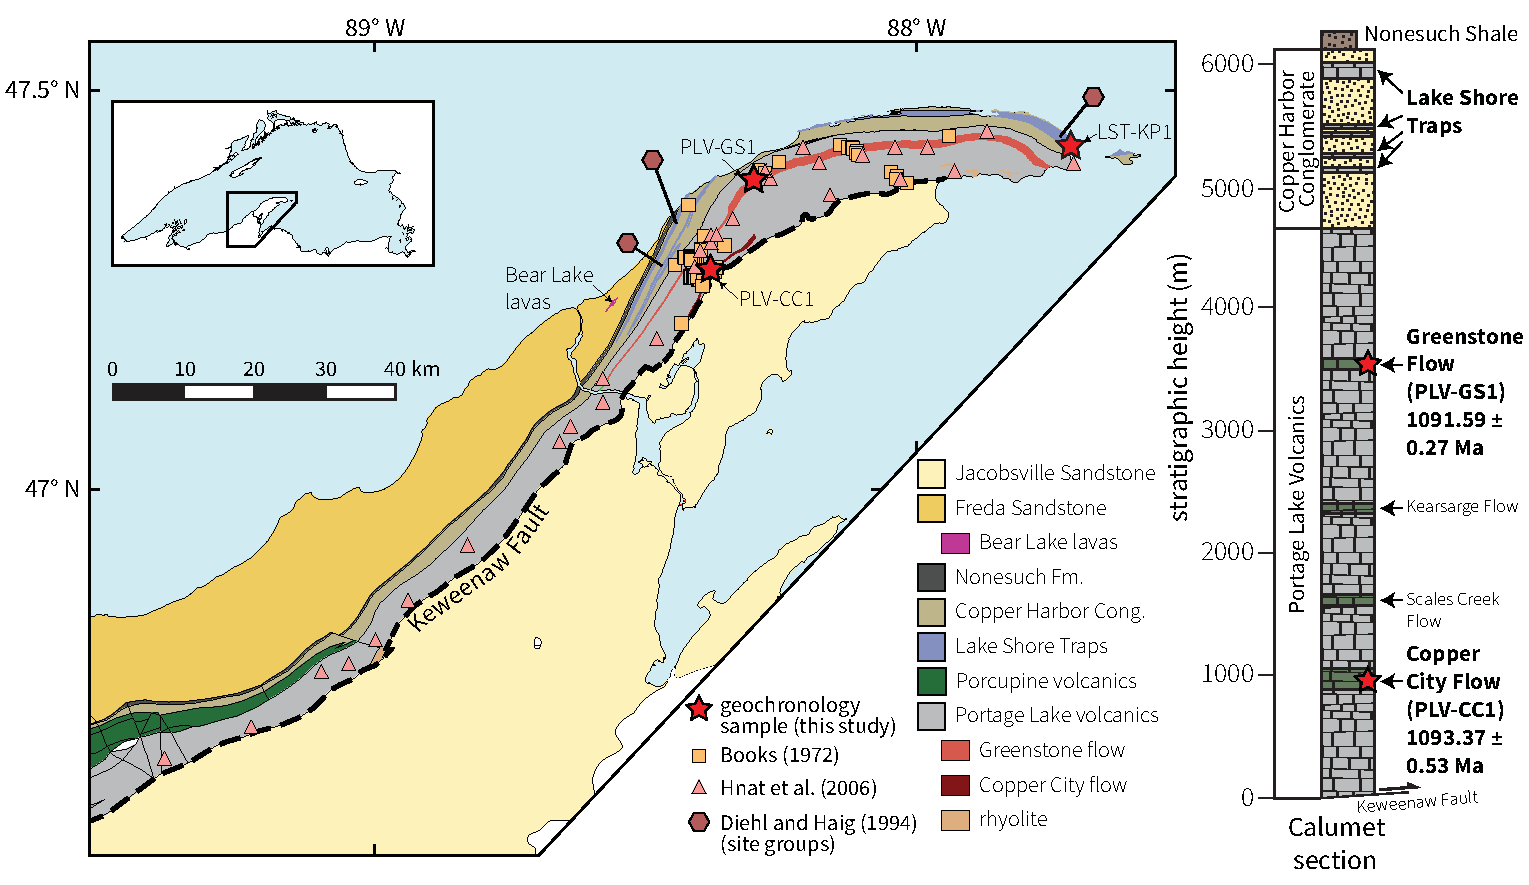
\includegraphics[width=6.5 in]{Figures/Fig7_PLV_map.pdf}
\caption{\small{\textbf{Geological map of the Keweenaw Peninsula, northern Michigan, and summary stratigraphy of the Portage Lake Volcanics and Copper Harbor conglomerate from a section near Calumet both modified from \cite{Cannon2001a}. The position of paleomagnetic sites from \cite{Books1972a} and \cite{Hnat2006a} used for the Portage Lake Volcanics pole and the localities of \cite{Diehl1994a} site groupings within the Lake Shore Traps are shown. The U-Pb dates shown for the Copper City Flow and the Greenstone Flow are from this study.}}}
\label{fig:PLV_Map}
\end{figure}

Atop the Portage Lake Volcanics are sedimentary rocks of the Copper Harbor Conglomerate which is the lowermost formation of the Oronto Group (Fig. \ref{fig:PLV_Map}). Within the Copper Harbor Conglomerate are basaltic to andesitic lava flows known as the Lake Shore Traps (Fig. \ref{fig:PLV_Map}; \citealp{Lane1907a}). These flows are concentrated into groupings within the conglomerate and were categorized into three flow clusters by \cite{Diehl1994a}: lower lava flows of the middle Lake Shore Traps, upper lava flows of the middle Lake Shore Traps and flows of the outer Lake Shore Traps. Paleomagnetic data were published from these flows by \cite{Diehl1994a} and \cite{Kulakov2013a}. The virtual geomagnetic poles from the Lake Shore Traps are grouped within three clusters as discussed in \cite{Diehl1994a} such that their distribution is non-Fisherian (Fig. \ref{fig:VGP}). The data of \cite{Kulakov2013a} added data from the easternmost cluster of middle Lake Shore Traps pulling the pole to the east (Fig. \ref{fig:VGP}). Following the interpretation of \cite{Diehl1994a} that the mean of the clusters provides a better positioning of the pole than each individual cluster, and given that a single cluster was heavily weighted by \cite{Kulakov2013a}, we use the pole position of \cite{Diehl1994a} in the compilation (180.8\textdegree E, 22.2\textdegree N, A95: 4.5\textdegree, N: 30; Fig. \ref{fig:VGP}; Table \ref{tab:poles}).

Overlying the Copper Harbor Conglomerate are the sedimentary rocks of the Nonesuch and Freda Formations (Fig. \ref{fig:PLV_Map}). Paleomagnetic data from the Nonesuch Formation and the lower 700 meters of the Freda Formation were developed by \cite{Henry1977a} and the calculated paleomagnetic poles for each formation are used for this compilation of the Keweenawan Track (Table \ref{tab:poles}). These pole positions are relatively insensitive to inclination shallowing as the shallow paleomagnetic directions of the data sets have shallow downwards and shallow upwards inclinations such that unflattening of both cancels out. In terms of the interpreted age of the units, new field mapping of the Bear Lake Felsite within the Freda Formation (Fig. \ref{fig:PLV_Map}) has revealed that it is a sequence of lava flows. While efforts to separate zircon from the flows has been unsuccessful, the presence of the volcanics suggests that deposition of the Freda Formation initiated while regional magmatism was still ongoing. The conformable nature of the Nonesuch Formation with the underlying Copper Harbor Conglomerate and the overlying Freda Formation are consistent with the Nonesuch Formation and basal portion of the Freda Formation having been deposited within the rift basin temporally close to the youngest dated volcanics (Fig. \ref{fig:chronostrat}).

\subsubsection{Geochronology}

Within the thickest lava flows of the Portage Lake Volcanics are pegmatoid horizons enclosed within ophitic basalt and dominantly comprised of coarse grained plagioclase and clinopyroxene with abundant magnetite and ilmenite. The pegmatoid layers are interpreted to have formed from partially differentiated, late-stage residual melt in the flow interior \citep{Longo1984a} and they typically contain zircon. \cite{Davis1990a} reported $^{207}$Pb/$^{206}$Pb dates developed from zircons in the pegmatoid layers of the Copper City Flow (1096.2 $\pm$ 1.8 Ma) and the Greenstone Flow (1094.0 $\pm$ 1.5 Ma). New data from 3 analyses of zircon separated from pegmatoid of the Copper City Flow (collected as sample PLV-CC1) yield a weighted mean $^{206}$Pb/$^{238}$U date of 1093.37 $\pm$ 0.53/0.69/1.4 Ma (MSWD of 0.33; Fig. \ref{fig:geochron}; Table \ref{tab:geochron}). Five zircon analyses from the Greenstone Flow pegmatoid (collected as PLV-GS1) yield a weighted mean $^{206}$Pb/$^{238}$U date of 1091.59 $\pm$ 0.27/0.52/1.3 Ma (Fig. \ref{fig:geochron}; Table \ref{tab:geochron}). The paleomagnetic pole calculated for the Portage Lake Volcanic is well-constrained by these new Copper City Flow and the Greenstone Flow dates.

Our new CA-ID-TIMS geochronology allows the eruption and subsidence analysis of \cite{Davis1990a} to be revisited. We approach this analysis by doing a Monte Carlo sampling of dates from their underlying distribution and calculate the implied eruption rate from these simulated date pairs using a thickness of 2850 meters between the flows. This analysis gives a median eruption rate of 1.6 mm/yr with a lower bound of 1.2 mm/yr and an upper bound of 2.4 mm/yr at 95$\%$ confidence. This fast rate of flow accumulation and associated subsidence supports other lines of evidence (e.g. \citealp{Fairchild2017a}) that active rift development was ongoing until at least 1092 Ma. The same analysis on the southwest sequence of the North Shore Volcanic Group yields similar rates with a median eruption rate of 2.1 mm/yr with a lower bound of 1.9 mm/yr and an upper bound of 2.5 mm/yr at 95$\%$ confidence.

The precision of the new geochronology now reveals that there is little temporal overlap in the accumulation of flows within the North Shore Volcanic Group and the Portage Lake Volcanics on the Keweenaw Peninsula (Fig. \ref{fig:chronostrat}). Following the eruption of the North Shore Volcanic Group there was a shift in the locus of subsidence and volcanism. The majority of the Portage Lake volcanics erupted during the period of time now represented by the unconformity between the North Shore Volcanic Group and the Schroeder-Lutsen basalts which are constrained to have erupted after the Greenstone Flow.

\subsection{Powder Mill Group}

\subsubsection{Background and Paleomagnetism}

The Powder Mill Group comprises the oldest volcanic rocks on the south shore of Lake Superior and underlies the Portage Lake Volcanics (Figs. \ref{fig:MCR_Map}, \ref{fig:chronostrat} and \ref{fig:PMG_Map}; \citealp{Palmer1986a,Nicholson1997a}). The Powder Mill Group is split into the Siemens Creek Volcanics, which are comprised of $\sim$2000 m of thin basalt flows, and the overlying Kallander Creek Volcanics, which are comprised of volcanic rocks ranging in composition from basalt to rhyolite  \citep{Palmer1986a, Cannon1996a}. The thickness of the Kallander Creek Volcanics is more difficult to estimate given variable thickness and the presence of the intrusive Mellen Complex, but it likely exceeds 6000 m near Kimball, Wisconsin. The uppermost lava flow in the Kallander Creek Volcanics is a quartz and feldspar-phyric rhyolite that is informally known as the Sheep Farm rhyolite \citep{Cannon1996a}. In the vicinity of Ironwood, Michigan and the Montreal River, the Kallander Creek Volcanics are overlain by the Portage Lake Volcanics followed by the Porcupine Volcanics and then the Copper Harbor Conglomerate (northernmost Wisconsin east in Figure \ref{fig:chronostrat}; Fig. \ref{fig:PMG_Map}). To the west, the Porcupine Volcanics and Portage Lake Volcanics are progressively missing such that at Brownstone Falls along the Bad River the unconformity is such that the Copper Harbor Conglomerate is directly atop the Sheep Farm rhyolite (northernmost Wisconsin west in Figure \ref{fig:chronostrat}; Fig. \ref{fig:PMG_Map}). Structural measurements on the upper Kallander Creek Volcanics and the unconformably overlying Oronto Group sedimentary rocks along the Tyler Forks and Bad Rivers on either side of Brownstone Falls reveal that this unconformity, termed the Brownstone Falls unconformity in Figure \ref{fig:chronostrat}, has angular discordance such that the time of Oronto Group deposition the Kallander Creek volcanics were locally dipping $\sim$40\textdegree$\;$to the northeast.

\begin{figure}[!h]
\centering
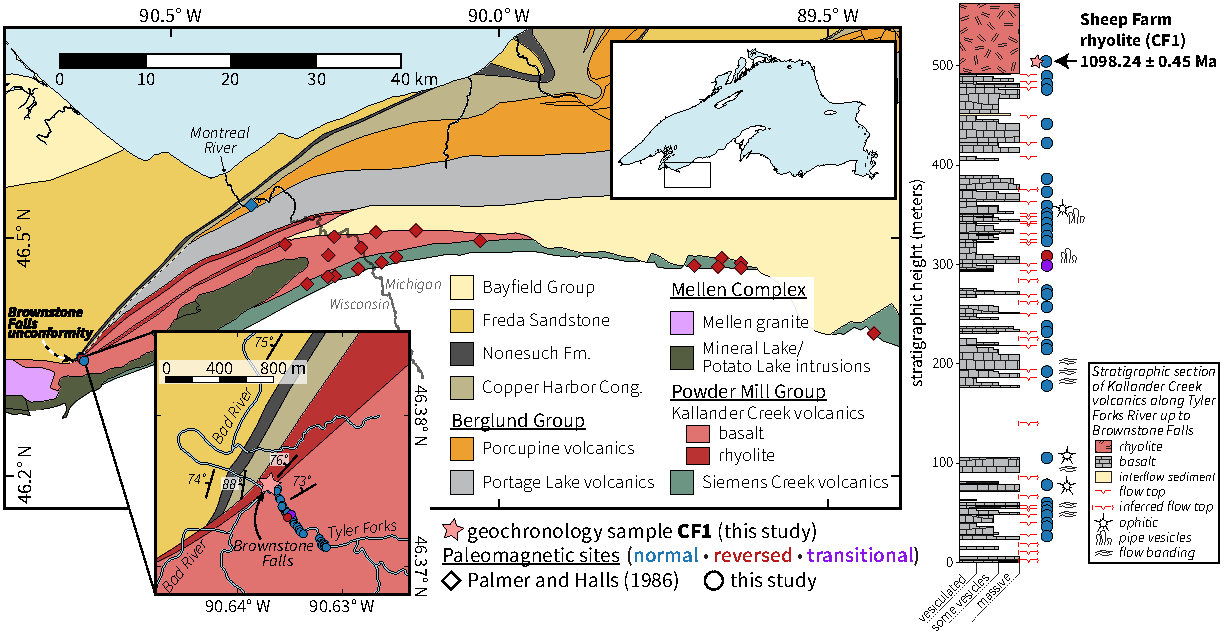
\includegraphics[width=6.5 in]{Figures/Fig8_PMG_map.pdf}
\caption{\small{\textbf{Geological map modified from \cite{Cannon1996a} focused on the Powder Mill Group in northern Wisconsin and the westernmost part of Michigan's upper Peninsula. The position of paleomagnetic sites deemed to have primary remanence from \cite{Palmer1986a} and those from this study are shown. The zoom-in map is centered Brownstone Falls within Copper Falls State Park and shows the location of the upper Kallander Creek Volcanics sites of this study and the Sheep Bed rhyolite geochronology sample. The stratigraphic column is of the upper 560 meters of the Kallander Creek Volcanics measured where the volcanics were sampled along the Tyler Forks River.}}}
\label{fig:PMG_Map}
\end{figure}

Paleomagnetic data previously developed from the Powder Mill Group have targeted the Siemens Creek Volcanics and the lower portion of the Kallander Creek Volcanics revealing dominantly reversed polarity (Fig. \ref{fig:PMG_Map}; \citealp{Books1972a,Palmer1986a}. The study of \cite{Palmer1986a} found that the four sites they studied that had normal polarity (one of which spanned the lower 150 meters of the Siemens Creek Volcanics) were associated with pervasive amphibole development and partial obliteration of original igneous texture. As a result, they suggested that these sites had been remagnetized through localized metamorphism during the Portage Lake Normal Polarity Zone. This result removed a pole determined from normally magnetized sites in the lowermost Siemens Creek Volcanics by \cite{Books1972a} that \cite{Halls1982a} had used to define an ascending arm up to the Logan Loop early in the history of rift volcanism. Instead, the pole positions from the ca. 1140 Ma Abitibi dikes \citep{Ernst1993a} and coeval ca. 1144 Ma lamprophyre dikes \citep{Piispa2018a}, as well of those of ca. 1160 Ma intrusions from southern Greenland \citep{Piper1992a, Upton2013a}, indicate that Laurentia was at high latitudes, and at a near standstill, prior to the Keweenawan Track (Fig. \ref{fig:MCR_Map}). Based on geophysical surveys conducted in the field, \cite{Nicholson1997a} suggested that there are also normally magnetized flows near the top of the Powder Mill Group in the upper Kallander Creek Volcanics immediately underlying the Sheep Farm rhyolite at the top of that unit. To evaluate these field survey data, we collected paleomagnetic samples from 35 lava flows in the uppermost 560 meters of the Kallander Creek Volcanics and developed alternating field (AF) demagnetization data (Fig. \ref{fig:PMG_Map}). AF demagnetization was variably successful in removing remanence from the samples as the result of varying dominance of magnetite and hematite. These data reveal that the flows, including the Sheep Farm rhyolite, are dominantly of normal polarity. The exception are two lava flows 170 to 198 meters below the Sheep Bed rhyolite (sites CF16 and CF17; Fig. \ref{fig:PMG_Map}). Site CF16 is of reversed-polarity and the lava below it (site CF17) has a transitional direction removed by AF demagnetization as well as a high coercivity remanence of reversed polarity likely corresponding to hematite that formed as the overlying reversed-polarity flow was emplaced. This transitional direction is similar to that see in the three flows below the start of the Flour Bay reversed-polarity zone in the Mamainse Point succession \citep{Swanson-Hysell2014a}. Below these lavas are another 18 analyzed flows within $\sim$300 meters of stratigraphy that all have normal polarity (Fig. \ref{fig:PMG_Map}). The reversed polarity CF16 flow could correspond with the Flour Bay reversed-polarity zone. However, given that it is a thin stratigraphic interval it is possible that it is associated with a brief reversed subchron early in the Portage Lake normal-polarity zone. The Kallander Creek Volcanics should be a target of future paleomagnetic study to further elucidate their polarity record including determining the position within the volcanics of the reversal from the Alona Bay reversed-polarity zone to the Flour Bay reversed-polarity zone.

The paleomagnetic data of \citet{Palmer1986a} included sites within both the Siemens Creek and Kallander Creek Volcanics. The researchers divided the data into three groups based on the structural panel from which they were sampled. One of the groups, with sites all within the Siemens Creek Volcanics, comes from a shallower dipping panel than the other two and the authors are more confident that it can be properly structurally corrected (``most reliable structural panel'' VGPs in Fig. \ref{fig:VGP}). A complication with structural correction in the more steeply dipping portions of the Powder Mill Group is that there were two significant and distinct tilting events. The first tilting occurred during rift development and led to the significant angular unconformity between the Kallander Creek Volcanics and the overlying Oronto Group sediments seen at Brownstone Falls. The second tilting was during the development of the Montreal River monocline which led to the near vertical dips of the Oronto Group \citep{Cannon1993a}. This complexity leads to uncertainty associated with tilt-correction and decreased confidence in declination of the site means and ultimately the pole position. We therefore follow the approach of \citet{Palmer1986a} and restrict the calculation of a pole to the subset of VGPs which come from a shallowly dipping structural panel within the Siemens Creek Volcanics (214.0\textdegree E, 45.8\textdegree N, A95: 9.2\textdegree, N: 10; Fig. \ref{fig:VGP}; Table \ref{tab:poles}).

\subsubsection{Geochronology}

\cite{Davis1997a} reported a $^{207}$Pb/$^{206}$Pb date of 1107.3 $\pm$ 1.7 Ma based on three multi-grain fractions from a felsic volcanic unit within the Kallander Creek Volcanics. \cite{Zartman1997a} obtained a multi-grain $^{207}$Pb/$^{206}$Pb date of 1098.8 $\pm$ 1.9 Ma for the Sheep Farm rhyolite at the very top of the Kallander Creek Volcanics. \cite{Zartman1997a} also reported $^{207}$Pb/$^{206}$Pb dates from samples of the Mellen Intrusive Complex that has been interpreted to be cogenetic with the upper Kallander Creek Volcanics \citep{Cannon1993b}: a date of 1102.0 $\pm$ 2.8 Ma for granophyre within the Mineral Lake intrusion and 1100.9 $\pm$ 1.4 Ma for the Mellen granite which cross-cuts the Mineral Lake intrusion (Fig. \ref{fig:PMG_Map}). Paleomagnetic data developed by \cite{Books1966a} show the Mineral Lake intrusion to have normal polarity.

 In order to develop a higher precision constraint on the chronostratigraphy of the Powder Mill Group, we developed new data for the Sheep Farm rhyolite with four zircon analyses from sample CF1 yielding a weighted mean $^{206}$Pb/$^{238}$U date of 1098.24 $\pm$ 0.45/0.63/1.3 Ma (Fig. \ref{fig:geochron}; Table \ref{tab:geochron}). Given that this flow is of normal polarity, as are 14 additional flows in the 170 meters of stratigraphy below it (Fig. \ref{fig:PMG_Map}), we consider this date to be within the early portion of the Portage Lake normal-polarity zone (Fig. \ref{fig:geochron}). That this date from the top of the Kallander Creek volcanics is only $\sim$2 Myr younger than the MP111-182 date from within the Flour Bay reversed-polarity at Mamainse Point suggests that the Kallander Creek Volcanics were erupting during the Flour Bay polarity zones. This interpretation would be consistent with the normally-magnetized Mineral Lake intrusion of the Mellen Complex being emplaced during the Flour Bay normal-polarity zone, but precise CA-ID-TIMS $^{206}$Pb/$^{238}$U dates and additional paleomagnetic analyses are required to make such an interpretation with confidence. The pole from the Siemens Creek Volcanics comes from units that are older than all of these dated units and corresponds to the Alona Bay Reversed Polarity Zone (Figs. \ref{fig:geochron} and \ref{fig:chronostrat}).

\subsection{Michipicoten Island Formation}

\subsubsection{Background and Paleomagnetism}

The Michipicoten Island Formation comprises late stage lava flows and tuffs that outcrop on Michipicoten Island in northeastern Lake Superior (Fig. \ref{fig:MCR_Map}). The formation was mapped in detail by \cite{Annells1974a} who split it into members dominated by differing volcanic lithologies including mafic, intermediate and felsic lavas and lithic tuffs. Many of the lavas in the formation are quite thick which limits the total number of exposed cooling units that can be sampled for paleomagnetism. \cite{Fairchild2017a} took the approach of developing data from 20 of the relatively thin mafic lavas of the South Shore Member and combined these data with data from three additional flows of \citet{Palmer1987a} for the development of a Michipicoten Island Formation paleomagnetic pole (174.7\textdegree E, 17.0\textdegree N, A95: 4.4\textdegree, N: 23; Fig. \ref{fig:VGP}; Table \ref{tab:poles}). This pole position falls on a progression from older paleomagnetic poles developed from volcanics and those obtained from the rift-related sedimentary formations that were deposited in the basin at the end of regional volcanism. Such a pole position is consistent with the interpretation, supported by geochronology, that the Michipicoten Island Formation comprises some of the youngest volcanics in the Midcontinent Rift (Fig. \ref{fig:chronostrat}).

Stratigraphically below the Michipicoten Island Formation and a thick package of hypabassal intrusions is a sequence of sub-ophitic to ophitic olivine tholeiitic basalt flows of the Quebec Mine Member. These flows were correlated by \cite{Annells1974a} to the main stage volcanics of the Mamainse Point Formation, but these thick ophites also bear physical resemblance to other main stage volcanics such as the Portage Lake Volcanics. The paleomagnetic data of \cite{Palmer1987a} include 8 sites from within these flows. Once one apparent outlier is excluded, these data yield a pole position (185.6\textdegree E, 36.9\textdegree N, A95: 13.4\textdegree, N: 7; Fig. \ref{fig:VGP}; Table \ref{tab:poles}) that is broadly consistent with other data from the Portage Lake normal-polarity zone, but the VGPs are scattered compared to other data from rift volcanics. This low precision, combined with the low number of sites, renders this pole of little use until more data are developed.

\subsubsection{Geochronology}

Age constraints for the Michipicoten Island Formation come from $^{206}$Pb/$^{238}$U zircon dates for the West Sand Bay Member tuff (1084.35 $\pm$ 0.20/0.34/1.2 Ma) and the Davieaux Island rhyolite (1083.52 $\pm$ 0.23/0.35/1.2 Ma; Fig. \ref{fig:geochron}; Table \ref{tab:geochron}) reported in \cite{Fairchild2017a}. The Michipicoten Island paleomagnetic pole described above was developed such that all of the VGPs within the pole are bracketed by these dated extrusive units.

\subsection{Volcanic Successions in the Midcontinent Rift not in the compilation}

\subsubsection{Chengwatana Volcanics}

The Chengwatana Volcanics of west central Wisconsin are the southernmost surface exposure of Midcontinent Rift volcanics (Fig. \ref{fig:MCR_Map}). Paleomagnetic data from the Chengwatana Volcanics were developed by \cite{Kean1997a}. These paleomagnetic data are intriguing as they include both normal and reversed directions that could potentially be correlative to the Flour Bay polarity zones. However, the definition of a site within the study was broad sampling regions (often more than 1 km across) that encompass multiple lava flows \citep{Kean1997a}. It is therefore not possible to calculate flow level VGPs from these data as would be necessary to calculate a paleomagnetic pole.

\subsubsection{Cape Gargantua Volcanics}

The Cape Gargantua volcanics north of Mamainse Point lie unconformably on Superior Province basement (Fig. \ref{fig:MCR_Map}). These volcanics have been shown by \cite{Palmer1970a} and \cite{Robertson1973a} to record a reversal from reversed to normal polarity which is likely associated with the end of the Alona Bay reversed-polarity zone. Paleomagnetic poles for the succession are not included in this compilation given that data generated by \cite{Palmer1970a} were not reported at the site level and data from \cite{Robertson1973a} only come from three sites.

\begin{landscape}
\begin{table}
\caption[Keweenawan track poles]{Paleomagnetic poles compiled for the Keweenawan Track.}
\scriptsize
\begin{tabular}{p{3.5 cm}rrrrp{3.5 cm}rrrp{3.5 cm}}
\toprule
                                           Pole &  Pole lon &  Pole lat &  $A_{95}$ &   N &                                               Pole reference &  Age (Ma) &  Lower age (Ma) &  Upper age (Ma) &                                  Age reference \\
\midrule
 Osler reverse (lower) &  218.6 &  40.9 &  4.8 &  30 &  Swanson-Hysell et al., 2014b &  1108.00 &  1105.15 &  1110.00 &  Davis and Sutcliffe, 1985; this study \\
 \midrule
 Osler reverse (upper) &  203.4 &  42.3 &  3.7 &  64 &  Halls, 1974; Swanson-Hysell et al., 2014b; this study &  1105.15 &  1104.82 &  1105.48 &  this study \\
 \midrule
 Osler normal &  171.9 &  32.0 &  9.7 &  4 &  Halls, 1974; this study &  1095.00 &  1080.00 &  1100.00 &   \\
 \midrule
 Mamainse lower reversed 1 &  227.0 &  49.5 &  5.3 &  24 &  Swanson-Hysell et al., 2014a &  1109.00 &  1106.00 &  1112.00 &   \\
 \midrule
 Mamainse lower reversed 2 &  205.2 &  37.5 &  4.5 &  14 &  Swanson-Hysell, 2014a &  1105.00 &  1100.40 &  1109.00 &  Swanson-Hysell, 2014a \\
 \midrule
 Mamainse lower normal and upper reversed &  189.7 &  36.1 &  4.9 &  24 &  Swanson-Hysell, 2014a &  1100.36 &  1100.10 &  1100.61 &  Swanson-Hysell, 2014a \\
 \midrule
 Mamainse upper normal &  183.2 &  31.2 &  2.5 &  34 &  Swanson-Hysell, 2014a &  1094.00 &  1090.00 &  1100.00 &   \\
 \midrule
 Grand Portage Basalts &  201.7 &  46.0 &  6.8 &  13 &  Books, 1968; Tauxe and Kodama, 2009 &  1106.00 &  1105.28 &  1108.00 &  this study \\
 \midrule
 North Shore Volcanic Group (upper NE sequence) &  181.7 &  31.1 &  4.2 &  28 &  Books, 1972; Tauxe and Kodama, 2009 &  1095.00 &  1092.00 &  1098.00 &  Davis and Green, 1997; Fairchild et al., 2017 \\
 \midrule
 North Shore Volcanic Group (upper SW sequence) &  179.3 &  36.9 &  2.1 &  78 &  Tauxe and Kodama, 2009; this study &  1096.18 &  1093.94 &  1096.75 &  this study \\
 \midrule
 Schroeder Lutsen Basalts &  187.6 &  28.3 &  2.5 &  65 &  Books, 1972; Tauxe and Kodama, 2009; Fairchild et al., 2017 &  1090.00 &  1085.00 &  1091.50 &  Fairchild et al., 2017 \\
 \midrule
 Portage Lake Volcanics &  182.5 &  27.5 &  2.3 &  78 &  Books, 1972; Hnat et al., 2006 &  1092.51 &  1091.59 &  1093.37 &  this study \\
 \midrule
 Lake Shore Traps &  180.8 &  22.2 &  4.5 &  30 &  Diehl and Haig, 1994 &  1085.47 &  1084.00 &  1091.00 &  Fairchild et al., 2017; this study \\
 \midrule
 Siemens Creek Volcanics &  214.0 &  45.8 &  9.2 &  10 &  Palmer and Halls, 1986 &  1108.00 &  1105.00 &  1111.00 &  Davis and Green, 1997 \\
 \midrule
 Quebec Mine Member (Michipicoten Island) &  185.6 &  36.9 &  13.4 &  7 &  Palmer and Davis, 1987 &  1095.00 &  1086.50 &  1100.00 &  Palmer and Davis, 1987 \\
 \midrule
 Michipicoten Island Formation &  174.7 &  17.0 &  4.4 &  23 &  Palmer and Davis, 1987; Fairchild et al., 2017 &  1083.95 &  1083.52 &  1084.39 &  Fairchild et al., 2017 \\
 \midrule
 Nonesuch Formation &  178.1 &  7.6 &  5.6 &  11 &  Henry et al., 1977 &  1080.00 &  1070.00 &  1083.50 &  see discussion in text \\
 \midrule
 Freda Formation &  179.0 &  2.2 &  4.2 &  20 &  Henry et al., 1977 &  1070.00 &  1060.00 &  1083.50 &  see discussion in text \\
\bottomrule
\end{tabular}
Notes: Pole lat and Pole lon give the latitude and longitude of the mean pole position, and A$_{95}$ gives the 95\% confidence ellipse for the pole. N indicates how many site mean VGPs were used for the calculation of the pole. The estimated ages of the paleomagnetic poles are shown with estimated lower and upper bounds which are particularly tightly constrained for poles associated with, or bracketed by, $^{206}$Pb/$^{238}$U dates. $^{207}$Pb/$^{206}$Pb dates from \cite{Davis1985a}, \cite{Palmer1987a} and \cite{Davis1997a} are not directly comparable to the $^{206}$Pb/$^{238}$U dates, but provide less precise constraints on additional poles.
\label{tab:poles}
\end{table}
\end{landscape}

\section{Discussion}

\subsection{The Keweenawan Track and implied rates of motion}

Often in dealing with Precambrian poles there is a sparsity of data such that poles are widely spaced temporally and spatially. Given the abundance of data from the Midcontinent Rift this is not the case, and we are in a situation where it would be advantageous to transform the poles into a synthesized apparent polar wander path (APWP). The goal of mean APWPs is to combine poles into a single path and to reduce potentially spurious motion that would occur if every mean pole position were utilized for paleogeographic reconstruction.

\subsubsection{Existing approaches for developing apparent polar wander paths}

The development of APWPs in the Phanerozoic is commonly done by calculating a running mean of the poles or by fitting a spherical spline to them \citep{Torsvik2008a,Torsvik2012a}. As typically implemented, both approaches require that poles are assigned absolute ages. The running mean approach takes all the poles whose age falls within a defined window and calculates the Fisher mean of those poles giving each pole equal weight. The mean is then taken to be the representative pole position for a continent at a given time with the associated A$_{95}$ having ambiguous meaning, but overall giving insight into the number of poles in the mean and how tightly they are clustered. The moving window approach that has typically been applied for running mean paths is to use a 20 Myr window to calculate mean poles every 10 Myr (e.g. \citealp{Torsvik2012a}). However, with certain data sets and intervals of time there can be over-smoothing with a window of this duration such that shorter duration bins are sometimes put into use (e.g. \citealp{Torsvik2008a}). An advantage of the running mean approach is that it is easily reproducible. A difficulty of the approach is that it is most effective when there are many poles in each time bin which can lead to increasing the duration of the windows. Increasing the duration of the running mean window can lead to smoothing that has the potential to eliminate real motion along a path. Running mean poles for this compilation of the Keweenawan Track are shown in Figure \ref{fig:mean_APWP} and Table \ref{tab:APWP}.

\begin{figure}
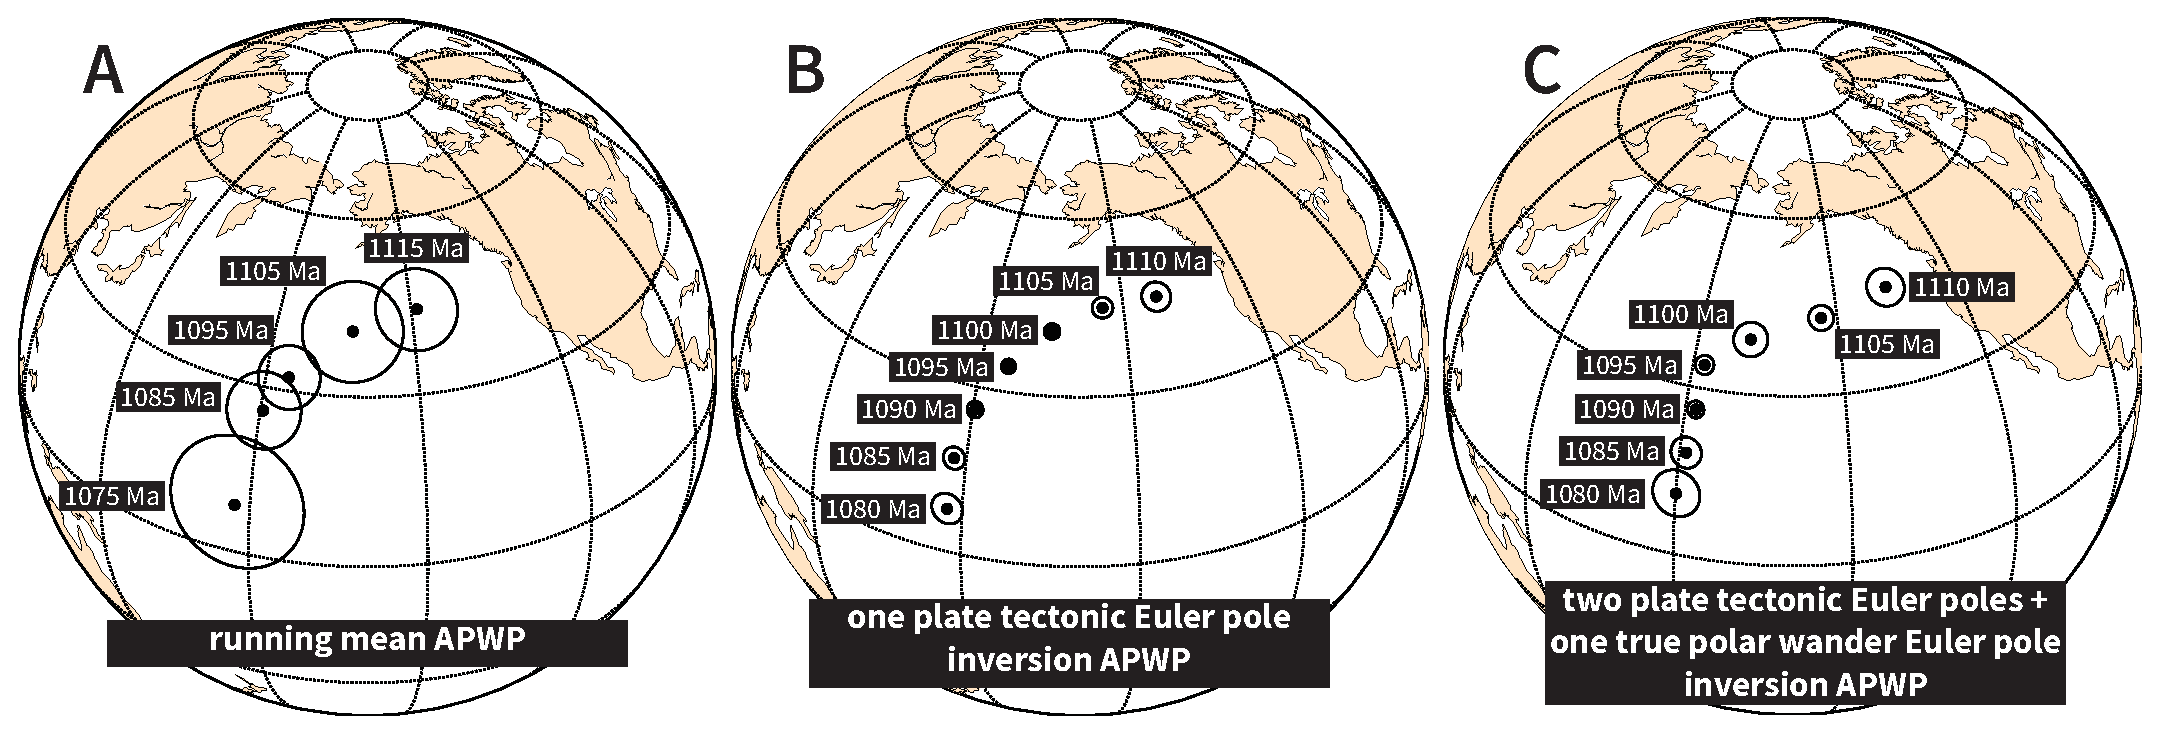
\includegraphics[width=\textwidth]{Figures/Fig9_mean_APWP.pdf}
\caption{\small{\textbf{Synthesized stage poles associated with apparent polar wander paths for the Keweenawan Track. A: Running mean poles. B: 1 Euler pole inversion. C: 2 plate tectonic Euler pole + 1 true polar wander Euler pole inversion.}}}
\label{fig:mean_APWP}
\end{figure}

The spherical spline approach, initially developed by \cite{Jupp1987a}, fits a smooth curve to data points. When fitting a spline, a smoothing factor needs to be assigned and data points can be weighted on various criteria such as the certainty of the pole position or other factors such as the quality (Q) factor of a pole \citep{Van-der-Voo1990a}. As explained in \cite{Torsvik2008a}, weighting splines by the Q factor produces APWPs that are anchored to the most reliable poles, but does not provide angular uncertainty on the spline path itself.

The Paleomagnetic Euler Pole (PEP) method is another approach to fitting APW paths in which small circles are fit to the data \citep{Gordon1984a}. Any plate motion that can be described by a single Euler pole should result in poles lying along a small circle. The long continuous and curvilinear shape of oceanic fracture zones and hot spot tracks have been argued to support the interpretation that plate motions can be consistent over timescales of tens of millions of years \citep{Gordon1984a, Tarling1996a}. This framework led \cite{Gordon1984a} to propose that one should find the best-fit paleomagnetic Euler pole to a set of paleomagnetic poles. In this method, maximum likelihood criteria are used to establish goodness of fit such that the best fit paleomagnetic Euler pole and a 95$\%$ confidence ellipse on that pole can be reported. This method can be weighted on the basis of the A$_{95}$ uncertainty of the poles.

In addition to the uncertainty related to the position of a paleomagnetic pole (typically expressed as the A$_{95}$ confidence ellipse), there is uncertainty associated with the age of the pole. None of the above methods provide a straightforward way of incorporating the age uncertainty of paleomagnetic poles. \cite{Jupp1987a} noted that for the spherical spline method: ``it should be observed that in examples such as this one [APWP], the data times are seldom known exactly, but are measured with error. Thus, strictly speaking, the spline solution is inappropriate. It would be better to use a spline-based theory of structural relationships. Unfortunately, such a theory does not yet exist.''

\subsubsection{A Bayesian paleomagnetic Euler pole inversion approach to APWP development}

It would be preferable to fit APWPs to data in a way that considers both the positional and temporal uncertainty of the paleomagnetic poles. We have developed such a method, in which we take a Bayesian approach to invert for the paleomagnetic Euler pole problem of \citet{Gordon1984a} using Markov-Chain Monte Carlo numerical methods. This approach provides a range of possible Euler pole solutions (each with three parameters: a latitude, a longitude, and a rotation rate), given the ages and positions of the paleomagnetic poles. The uncertainties in pole position and age are incorporated into the inversion for the paleomagnetic Euler poles. The inversion can be set up to invert for one or multiple Euler poles; in the latter case the timing of the changepoint from one Euler pole to another is an additional unknown that is solved for as part of the inversion.  An additional advantage of this approach is that the resulting paleomagnetic Euler poles provide an estimate for the total plate velocity, rather than just the latitudinal component of motion. This estimate of the total velocity is possible because both the latitudinal change and the rotation of the continent recorded in the paleomagnetic pole progression are being fit with an Euler pole, so the resulting angular vector constrains both latitudinal and longitudinal motion. The solutions that emerge from the inversion provide this velocity estimate as well as the associated uncertainty. The code that implements the inversion does so through a Markov-Chain Monte Carlo approach and is openly available within a Github repository associated with this work.

The Keweenawan Track pole compilation includes poles that are tightly constrained in time by radiometric dates, as well as poles that have looser constraints (Table \ref{tab:poles}; Fig. \ref{fig:bayesian_1_euler}). In a Bayesian framework, each unknown being inverted for is assigned a prior probability distribution. The ages of the paleomagnetic poles are one such unknown. When intimately associated with a radiometric date, the ages of the poles were assigned a Gaussian distribution. When age bounds came from looser stratigraphic bracketing or polarity zone constraints, the ages of the poles were taken to come from a uniform distribution between the lower and upper ages in Table \ref{tab:poles}. These probability distributions for the pole ages are displayed graphically in Figure \ref{fig:bayesian_1_euler}D.

A one-Euler-pole inversion for the Keweenawan Track does an effective job fitting the pole path resulting in a mean Euler pole of 215\textdegree E, 9\textdegree N (Fig. \ref{fig:bayesian_1_euler}). The median plate rate estimate from the one Euler pole inversion is 31 cm/year with 95$\%$ of the rates (referred to as the credible interval) coming between 27-34 cm/yr (Fig. \ref{fig:bayesian_1_euler}).

\begin{figure}
\begin{centering}
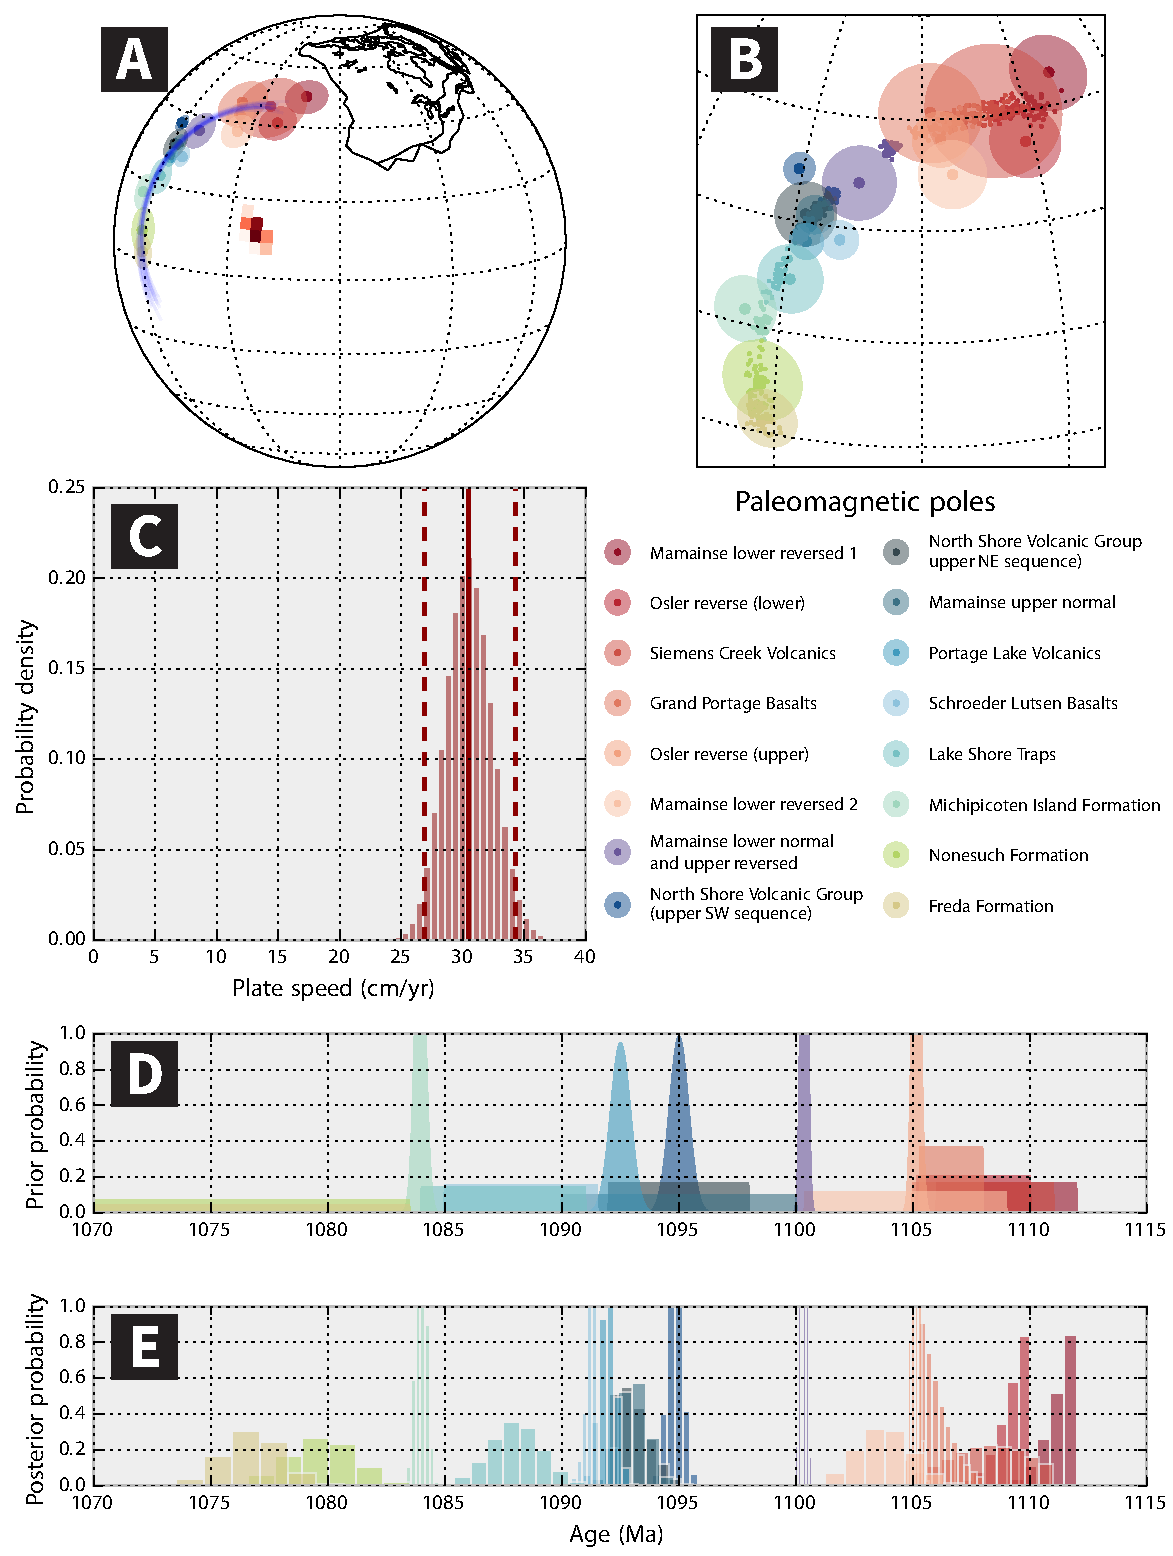
\includegraphics[width=0.85\textwidth]{Figures/Fig10_bayesian_1_euler.pdf}
\caption{\small{\textbf{Inversion of the Keweenawan track for a single Euler rotation using the Bayesian framework discussed in the text. A: Euler pole locations developed through the inversion shown as a density plot along with a representative resulting tracks drawn over the paleomagnetic poles. B: Paleomagnetic pole positions for draws from the posterior distribution of the inversion superimposed on observed pole positions and their uncertainty. C: Laurentia plate speed distribution from the inversions. The solid line shows the median plate speed (31 cm/yr) and the dashed lines show the 95\% credible interval (27-34 cm/yr). D: Prior probability distributions for the ages of the paleomagnetic poles. Poles with radiometric ages are given Gaussian prior distributions. Poles with stratigraphic age control are given uniform prior distributions between bracketing ages. E: Posterior probability distributions for the ages of the poles resulting from the inversion.}}}
\label{fig:bayesian_1_euler}
\end{centering}
\end{figure}

The motion of Laurentia manifest in the Keweenawan Track has been attributed both to:
\begin{itemize}
\item rapid differential plate tectonic motion---wherein the path is the result of the motion of Laurentian lithosphere relative to the asthenosphere, mesosphere (lower mantle) and other plates (as in \citealp{Davis1997a}).
\item rapid true polar wander (TPW)---wherein the path resulted from rotation of Earth's whole mantle with respect to the spin axis \citep{Evans2003b}.
\end{itemize}
That the motion from the Logan to Grenville Loop, which is captured in the Keweenawan Track, is the result of true polar wander factors significantly into the orthoversion model of supercontinent cyclicity and the associated reconstruction \citep{Mitchell2012a}. In that model, the Euler pole to a great circle fit from the Logan Loop to the Grenville Loop is taken to correspond to Earth's minimum inertial axis at the time, which is interpretted to be the ``true polar wander legacy'' of the Nuna supercontinent \citep{Evans2003b}. Rotations due to true polar wander should result in poles that trace out a great circle. To solely explain the Keweenawan Track as the result of true polar wander, we can modify the Bayesian inversion to be restricted to inverting the path as a great circle. This inversion is implemented by forcing the Euler pole to be 90\textdegree$\;$from the starting point of the path. Such an inversion does a poor job of fitting the entire path (Fig. \ref{fig:bayesian_results}). It is clear that the best fit to the pole swath is a small circle rather than a great circle (Figs. \ref{fig:bayesian_1_euler} and \ref{fig:bayesian_results}).

Though the whole Keweenawan Track cannot be adequately described by TPW, that does not rule out a combination of differential plate tectonic motion and TPW. Therefore, a more appropriate model is likely one wherein some component of the APWP is the result of true polar wander (and thereby a great circle) and another component is the result of differential tectonic motion (and thereby a small circle, although one solution would be a great circle). We therefore invert for both one plate tectonic Euler pole and one true polar wander Euler pole (Fig. \ref{fig:bayesian_results}). This model allows for a significant portion of the APWP to be ascribed to TPW, but the bulk of the track is still due to differential plate motion in the inversions, and a solution with zero TPW remains a good fit.  Therefore, while we can robustly conclude that the Keweenawan Track is not well-explained by true polar wander alone and can be well-explained by plate tectonics alone, it is possible that a portion of the motion is due to TPW. Even so, 97.5$\%$ of the solutions have small circle plate tectonic motion that is faster than 20 cm/year. That the rapid motion recorded in the Keweenawan Track precedes continental collision along leading margin of the continent is consistent with a significant component of the velocity being associated with differential plate tectonic motion (Fig. \ref{fig:cross_section}). The total speed resulting from the combination of TPW and differential plate tectonic motion is quite similar to the single Euler pole inversion with a median rate of 30 cm/year with a 95$\%$ credible interval of 27-34 cm/yr.

\begin{figure}
\begin{centering}
\includegraphics[width=0.85\textwidth]{Figures/Fig11_bayesian_inversions.pdf}
\caption{\small{\textbf{Inversion of the Keweenawan Track using four different models. Euler pole locations and sample tracks are shown for each inversion as are the paleomagnetic pole positions resulting from the inversion superimposed on observed pole positions (same color scheme as in Fig. \ref{fig:bayesian_1_euler}). The distribution of plate speeds attributable to each inverted Euler pole are shown in histograms with the 95\% credible interval indicated with dashed lines for each model.}}}
\label{fig:bayesian_results}
\end{centering}
\end{figure}

It has previously been argued that the Keweenawan Track records a slow-down in plate velocity in the late stage of Midcontinent Rift volcanism \citep{Davis1997a,Swanson-Hysell2009a}. \cite{Fairchild2017a} challenged this conclusion on the basis of a new paleomagnetic pole from the Michipicoten Island Formation which was interpreted to show continued rapid motion until 1083 Ma. If there was a slow-down, a single Euler pole inversion is not appropriate. To address this possibility, the pole path was fit with a two plate tectonic Euler pole inversion (Fig. \ref{fig:bayesian_results}). This inversion for two Euler poles is consistent with a hypothesized slow-down, but with a more minimal change than the slow-down from a latitudinal velocity of 22 cm/year to 8 cm/year proposed by \citet{Davis1997a}. The new two Euler pole inversion results in velocities at the high latitude portion of the track of 25 cm/yr (95$\%$ interval of 20 to 32 cm/yr) then changing at 1096 Ma (95\% interval of 1095-1099 Ma) to 19 cm/yr (95$\%$ interval of 11 to 31 cm/yr). As discussed below, the initiation of large-scale orogenesis associated with the Grenvillian orogeny provides a tectonic basis for a change in plate motion (Fig. \ref{fig:cross_section}).

Another model worth considering is one wherein there is constant true polar wander for the duration of the Keweenawan Track with plate tectonic motion associated with convergence between Laurentia and a conjugate continent that then changes with the initiation of collision. We explore this model with a combined inversion for two plate tectonic Euler poles with one overarching true polar wander Euler pole superimposed on top of it (Fig. \ref{fig:bayesian_results}). The results of this inversion are that the path can be well-explained by constant true polar wander of 14 cm/yr (95$\%$ interval of 5 to 22 cm/yr) with plate tectonic motion that starts at 15 cm/yr (95$\%$ interval of 7 to 25 cm/yr) and then changes at 1096 Ma (95\% interval of 1095-1099 Ma) to 4 cm/yr (95$\%$ interval of 0 to 19 cm/yr) (Fig. \ref{fig:bayesian_results}). In this inversion, the TPW pole and the second plate tectonic pole are in nearly the same location. This similarity in position results in significant tradeoffs between them, where a solution with fast TPW has slow plate speeds, and a solution with slow TPW speeds has fast plate speeds. The total motion in this inversion is 25 cm/year (95$\%$ credible interval of 20 to 32 cm/year) during the period of the first plate tectonic Euler pole that then slows to 17 cm/year (95$\%$ credible interval of 12 to 26 cm/year) following the changepoint.

When solving inverse problems, one must consider that adding more parameters to a model usually leads to a better fit, though the model may not be better from a theoretical or Occam's razor standpoint. That said, the inversions with two plate tectonic Euler poles do the best at fitting the data (especially for the Mamainse Point and North Shore Volcanic Group paleomagnetic poles) and is an intriguing solution given the dynamic and plate tectonic context. The resulting stage poles for this inversion are presented in Table \ref{tab:APWP} along with those for the running mean APWP and the inversion of a single plate tectonic Euler pole.

\begin{table}
\footnotesize
\caption{Synthesized apparent polar wander path stage poles for the Keweenawan Track}
\begin{tabular}{|l|llll|lll|lll|}
\hline
& \multicolumn{4}{l}{Running mean (20 Myr window)} & \multicolumn{3}{|l}{Bayesian PEP (1 plate} & \multicolumn{3}{|l|}{Bayesian PEP (1 true polar wander} \\
Age & \multicolumn{4}{l}{} & \multicolumn{3}{|l}{tectonic Euler pole)} & \multicolumn{3}{|l|}{+ 2 plate tectonic Euler poles)} \\
(Ma) & Plon (\textdegree) & Plat (\textdegree) & N & A$_{95}$ (\textdegree) & Plon (\textdegree) & Plat (\textdegree) & $\Theta_{95}$ (\textdegree) & Plon (\textdegree) & Plat (\textdegree) & $\Theta_{95}$ (\textdegree) \\
\hline
1115 & 211.3 & 44.0 & 6 & 6.8 &  &  &  &  &  &  \\
1110 & & & & &	218.2 & 45.4 & 2.5 &	222.7 & 46.3 & 3.2 \\
1105 & 195.5 & 40.0 & 12 & 7.9 &	205.2 & 44.7 & 1.7 &	206.4 & 42.7 & 2.1 \\
1100 & & &  &  &	193.9 & 40.7 & 1.3 &	191.1 & 39.0 & 2.8 \\
1095 & 184.5 & 32.2 & 10 & 5.3 &	185.6 & 34.2 & 1.2 &	182.3 & 33.9 & 1.6 \\
1090 & & & &  &	180.4 & 26.2 & 1.4 &	182.0 & 26.4 & 1.4 \\
1085 & 180.6 & 26.1 & 9 & 6.4 &	177.8 & 17.4 & 1.9 &	181.2 & 18.9 & 2.6 \\
1080 & & & & &	177.3 & 8.2 & 2.8 &	180.1 & 11.4 & 4.1 \\
1075 & 177.3 & 8.9 & 3 & 11.9 &  &  &  &  &  &  \\
\hline
\end{tabular}
\label{tab:APWP}
Notes: PEP: paleomagnetic Euler pole; $\Theta_{95}$ represents two angular standard deviations wherein 95$\%$ of the estimated path positions lie within that angle of the mean path position.
\end{table}

A more typical approach than this PEP inversion method for resolving how much of the change in pole position in a path is the result of true polar wander is to consider the APWP from other continents at the time that were not conjoined with the one of interest. Unfortunately, there are no contemporaneous paths that are comparable in terms of resolution and age-calibration to that of Laurentia. However, there are numerous paleomagnetic poles that are time-equivalent from the Kalahari Craton and the associated Sinclair terrane of present-day southern Africa. Poles have been developed from the ca. 1110 Ma Umkondo large igneous province \citep{Swanson-Hysell2015b}, the 1105.52 $\pm$ 0.41 Ma post-Guperas dikes \citep{Panzik2015a}, the $<$1108 $\pm$ 9 Ma Aubures Formation \citep{Kasbohm2015a} and the $\leq$1093 $\pm$ 7 Ma Kalkpunt Formation \citep{Briden1979a,Pettersson2007a}. These paleomagnetic poles all have similar positions to one another with the arc distance between the Kalkpunt Formation pole and the poles of the Umkondo large igneous province and post-Guperas dikes being less than that of time-equivalent Laurentia poles. This difference supports the interpretation that the pole position difference within the Keweenawan Track between 1110 and 1090 Ma has a component of rapid differential plate motion of Laurentia. However, the sense of motion along Kalahari's path is similar to that of the Keweenawan Track if Kalahari is reconstructed with the Namaqua-Natal Belt oriented towards the Grenville margin of North America \citep{Kasbohm2015a, Swanson-Hysell2015b}. The rate of TPW that results from the PEP inversion for one TPW and two plate tectonic Euler poles of the Keweenawan Track is consistent with the pole progression from the Kalahari craton.

\subsection{The transition from active rifting to thermal subsidence}

The timing of the transition from when the Midcontinent Rift basin was influenced by active extension to the post-rift interval when accommodation space was solely generated by thermal subsidence is of significant interest for understanding the history of rift development \citep{Cannon1992b,Stein2015a}. One line of argument for the timing of this transition is based on the lithofacies of the Oronto Group, with the widespread cobble-boulder conglomerates within the Copper Harbor Conglomerate interpreted to reflect alluvial-fan deposition that initiated during a time period of active fault-generated topography \citep{Elmore1984a, Zartman1997a}. In contrast, above the Copper Harbor Conglomerate and the lacustrine Nonesuch Formation, the Freda Formation is predominantly comprised of fluvial channel sandstones and overbank siltstones with conglomerate present only in the lower part of the formation within some successions \citep{Ojakangas2001a}. The Freda Formation was likely deposited within a broad low-gradient alluvial plain during the post-rift thermal subsidence phase of basin development \citep{Zartman1997a}. This lithofacies-based interpretation puts the syn- to post-rift transition within the Copper Harbor Conglomerate ca. 1086 Ma (Fig. \ref{fig:chronostrat}). Based on a crustal-scale cross-section informed by a deep seismic line from the GLIMPCE program, \cite{Cannon1992b} made a similar interpretation arguing that the last evidence for syn-depositional extension is within the very basal sedimentary units. In this interpretation, the majority of the volcanism was contemporaneous with active rifting, with the volumetrically more minor late stage volcanics of the Lake Shore Traps and the Michipicoten Island Formation post-dating active extension. A contrasting view was put forward in \cite{Stein2015a} wherein the end of active rifting occurred prior to the eruption of the Portage Lake Volcanics based on a reinterpretation of GLIMPCE seismic lines. In this interpretation, a more significant volume of volcanics within the Midcontinent Rift erupted during the post-rift phase of basin evolution.

Temporal constraints on angular unconformities can provide additional insight into the timing of this transition within a basin. In an active rift, rift-flank uplifts can arise associated with extension \citep{Braun1989a}. Subsequent thermal subsidence can lead to a post-rift unconformity as sediments being deposited in a thermally subsiding basin onlap onto eroded rift margins and flanks \citep{Braun1989a, Embry1990a, Bosence1998a}. While unconformities are also typical during the active syn-rift stage of basin development due to fault-driven differential subsidence and associated isostatic consequences, post-rift unconformities (sometime referred to as breakup unconformities) are particularly widespread \citep{Bosence1998a}. Post-rift unconformities can be particularly insightful for the timing of the end of rifting as they juxtapose underlying syn-rift strata with post-rift strata \citep{Embry1990a,Franke2013a}. The Brownstone Falls unconformity at which Oronto Group sedimentary rocks overlie progressively lower stratigraphic levels of the Porcupine Volcanics, Portage Lake Volcanics and Kallander Creek Volcanics, as seen in Figures \ref{fig:chronostrat} and \ref{fig:PMG_Map}, is well-explained as a post-rift unconformity. The volcanics underlying the unconformity could therefore be interpreted as syn-rift strata with the overlying Oronto Group having been deposited during widespread thermal subsidence. The syn-rift strata in this interpretation include the Portage Lake Volcanics which could constrain the post-rift phase to post-date 1091.59 $\pm$ 0.27/0.52/1.3 Ma. Another unconformity that is constrained with U-Pb geochronology is the angular unconformity between the upper southwest sequence of the North Shore Volcanic Group, along with the intrusive Beaver Bay Complex, and the overlying Schroeder-Lutsen Basalts (Figs. \ref{fig:chronostrat} and \ref{fig:NSVG_Map}). If the Schroeder-Lutsen Basalts are post-rift volcanics, this unconformity could also be considered as a post-rift unconformity. U-Pb dates of 1093.94 $\pm$ 0.28/0.52/1.3 Ma for the Palisade Rhyolite within the upper southwest sequence of the North Shore Volcanic Group and 1091.61 $\pm$ 0.14/0.30/1.2 Ma for an aplitic dike within the Beaver Bay Complex, put a similar age constraint on the timing of the syn- to post-rift transition as post-dating ca. 1091 Ma. Given these unconformity constraints and arguments based on sedimentary lithofacies, we consider the end of active extension within the rift to have most likely occurred between ca. 1091 and ca. 1086 Ma.

\subsection{The tectonic context of Midcontinent Rift development}

The margin of Laurentia to the present-day east of the Midcontinent Rift underwent polyphase orogenesis through the Mesoproterozoic (Fig. \ref{fig:cross_section}). The development of the Midcontinent Rift occurred within a time period of interpreted tectonic quiescence on that margin from ca. 1160 to 1090 Ma \citep{Rivers2008a, McLelland_ref}. Prior to this quiescence, there was accretionary orogenesis of the Shawinigan orogeny from ca. 1190 to 1160 Ma (Fig. \ref{fig:cross_section}; \citealp{McLelland_ref}). This orogeny has been interpreted to have resulted from the accretion of a terrane comprised of amalgamated arc volcanics and associated metasediments to the Laurentian margin \citep{McLelland_ref}. U-Pb zircon geochronology conducted on partial melts within metamorphic rocks, such as those in the Adirondack lowlands, provide temporal constraints on metamorphism associated with this accretionary orogenesis \citep{Heumann2006a}. The lack of deformation within the voluminous ca. 1155 Ma anorthosite-mangerite-charnockite-granite suite intrusives of the Adirondacks and elsewhere in the Grenville Province stands in contrast to ca. 1176-1162 Ma deformed plutons and has been inferred to constrain the cessation of Shawinigan deformation \citep{McLelland_ref}. The tectonic and magmatic quiescence that followed the Shawinigan orogeny implies that during the early stage of Midcontinent Rift volcanism the margin was not active (Fig. \ref{fig:cross_section}). There was local magmatism marked by the intrusion of the Hawkeye granite suite which was emplaced locally within the Adirondack Highlands Terrane and is temporally constrained by multigrain U-Pb TIMS upper intercept dates of 1100 $\pm$ 12 Ma, 1098 $\pm$ 4 Ma, 1095 $\pm$ 5 Ma, 1093 $\pm$ 11 Ma and 1089 $\pm$ 6 Ma \citep{Chiarenzelli1991a}. The overlap of the dates of this magmatic suite with the Midcontinent Rift has been hypothesized to be the result of a causal relationship \citep{McLelland_ref} and could be the result of melting associated with anomalously hot asthenosphere due to upwelling under Laurentian lithosphere. At ca. 1095 Ma, there was ongoing magmatic activity stretching across Laurentia from the Adirondack Highlands Terrane, through the Midcontinent Rift and throughout the Southwestern Laurentia large igneous province (Fig. \ref{fig:MCR_Map}; \citealp{Bright2014a}). Magmatism within the Southwestern Laurentia large igneous province appears to have spanned a similarly prolonged interval as magmatism within the Midcontinent Rift with dates spread between ca. 1100 and 1080 Ma \citep{Bright2014a}.

\begin{figure}
\centering
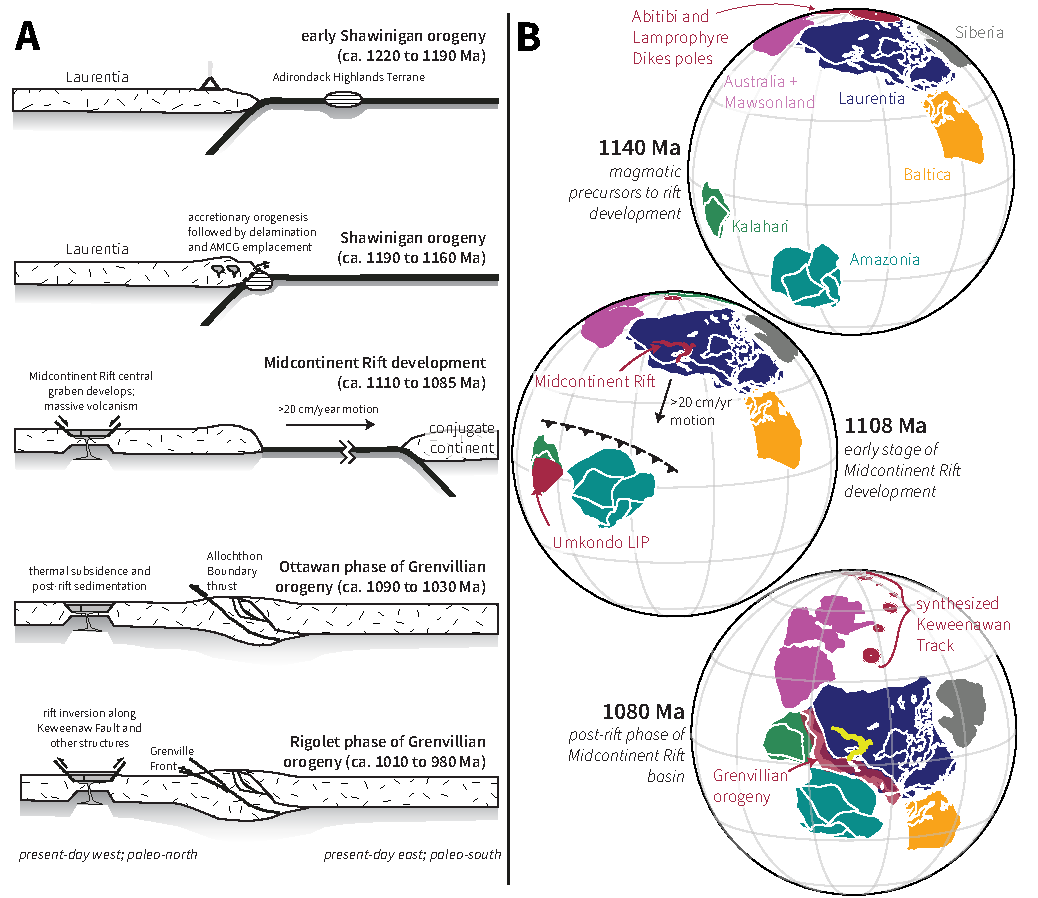
\includegraphics[width=6.5 in]{Figures/Fig12_cross-section_paleogeo.pdf}
\caption{\small{\textbf{A: Schematic cartoons of the development of the Midcontinent Rift in the context of Grenville margin orogenesis. The schematic transect extends from the interior of the Laurentia where the Midcontinent Rift developed to the margin of Laurentia in the vicinity of the modern day Adirondacks. The timescale and geometry of the Shawinigan orogeny follows that of \cite{Mclelland2013a}, while the timing and geometry of the Allochthon Boundary thrust and the Grenville Front follows that of \cite{Hynes2010a}. These cross-sections are schematic and not to scale. B: Paleogeographic reconstructions on an orthographic projection before, during and after active extension within the Midcontinent Rift. The positions of Baltica and Amazonia relative to Laurentia follows \cite{Evans2013b} with slight modifications. The ca. 1140 Ma reconstruction is consistent with the ca. 1150 Ma Fortuna Formation pole for Amazonia \citep{DAgrella-Filho2008a} and the ca. 1140 Ma Abitibi and lamprophyre dike poles of Laurentia \citep{Ernst1993a,Piispa2018a}. The position of Kalahari relative to Laurentia follows \cite{Swanson-Hysell2015b}, Australia relative to Laurentia follows \cite{Swanson-Hysell2012a} and Siberia relative to Laurentia follows \cite{Ernst2016a} and \cite{Evans2016b}.}}}
\label{fig:cross_section}
\end{figure}

Tectonic quiescence on the present-day eastern margin of Laurentia ended with the onset of the Ottawan phase of the Grenvillian orogeny which is typically interpreted to have started at 1090 Ma and continued to 1030 Ma \citep{McLelland2001a}. Note that this period of orogenesis is referred to both as the Ottawan orogeny (e.g. \citealp{McLelland2001a}) and as the Ottawan phase of the Grenvillian orogeny (e.g. \citealp{Rivers2008a}) wherein the Grenvillian orogeny also includes the Rigolet orogenic phase between ca. 1000 to 980 Ma (Fig. \ref{fig:cross_section}). There is also a tendency in the literature for the phrase ``Grenville orogeny'' to be broadly used to refer to any late Mesoproterozoic orogenesis on Laurentia's margins or those of other Proterozoic continents. Here, we restrict the use of ``Grenvillian orogeny'' to orogenesis along Laurentia's margin in the latest Mesoproterozoic and earliest Neoproterozoic (ca. 1090 to 980 Ma). Similarities in the timing of deformation, magmatism and metamorphism between the Grenville Province of Canada, the Adirondack Highlands of New York and the northern Blue Ridge Province of the Appalachians has been used to argue for extensive, in addition to prolonged, orogenesis at this time. Compilation of U-Pb zircon and monazite dates interpreted to record peak metamorphism have ages spanning largely from 1090 to 1050 Ma with ages from Ar-Ar dating of hornblende revealing cooling much later---from 990 to 950 Ma \citep{Rivers2008a}. These data have been used to develop a model wherein there was a long-lived orogeny with development of a thick orogenic plateau that subsequently gravitationally collapsed \citep{Rivers2008a}.

It has long been postulated that Midcontinent Rift development ceased as the result of far-field stresses associated with Grenville orogenesis \citep{Cannon1992a}. A contrasting model proposes that the Midcontinent Rift developed and then failed as a result of successful seafloor spreading along the present-day eastern margin of North America \citep{Stein2014a}. In this model, extension in the Midcontinent Rift ends when motion is accommodated by seafloor spreading between Laurentia and a conjugate continent. This model is difficult to reconcile with the temporal constraints of the Ottawan phase of Grenvillian orogenesis. \cite{Stein2014a} argued that the orogenic history of the Grenville Province in Canada may be erroneously being extrapolated into the continental United States. However, data from both the Adirondack Highlands Terrane and Grenville inliers through the Appalachians of the United States constrain high-grade metamorphism in that portion of the orogeny between ca. 1080 and 1050 Ma (McLelland et al., 2013). If a divergent plate boundary developed during Midcontinent rifting on that margin, it must have been short-lived and inverted soon after initiation given the record of collisional orogenesis.

In contrast to the high-precision U-Pb dates of volcanics from the Midcontinent Rift that can be obtained through CA-ID-TIMS, dates of Ottawan orogenesis can be complicated by the presence of polyphase growth that lead to zircon cores and rims of differing ages. These zircons are often better approached through techniques such as U-Pb dating through sensitive high-resolution ion microprobe (SHRIMP) techniques that can analyze portions of complexly zoned and polygenetic zircons, but do so at lower precision. Additionally, it is possible that the initiation of structural shortening associated with orogenesis could pre-date the formation of mineral phases that can be dated. Regardless, age constraints on the Midcontinent Rift and Grenville orogenesis have progressed such that the following summary statements can be made:
\begin{itemize}
\item Initiation of the Midcontinent Rift occurred during a period of relative tectonic quiescence on the Grenville margin. As a result, hypotheses that relate initiation of the Midcontinent Rift to far-field effects of Grenville collision (\textit{sensu stricto}) such as those proposed by \cite{Van-Schmus1985a} and \cite{Gordon1986a} are unlikely.
\item The cessation of extension within the Midcontinent Rift (after ca. 1091 Ma) is closely related in time with the onset of the Ottawan orogeny. This timing is consistent with hypotheses that postulate that Midcontinent Rift extension stopped due to lithospheric stresses associated with collisional orogenesis along the present-day eastern margin of North America.
\end{itemize}

Major structures within the Midcontinent Rift such as the Keweenaw Fault and the Douglas Fault were (re)activated during compression into reversed faults \citep{Cannon1992b}. However, whether the cessation of Midcontinent Rift extension was due to a change in lithospheric stress regime associated with Ottawan orogenesis need not imply that the timing of reverse-faulting along major structures such as the Keweenaw Fault occurred at the same time. The Grenvillian orogeny was quite protracted and it is the Rigolet phase of orogenesis (ca. 1000 to 980 Ma), rather than the Ottawan, that is hypothesized to have led to the development of the Grenville Front tectonic zone (Fig. \ref{fig:cross_section}; \citealp{Hynes2010a}). Earlier Ottawan orogenesis was concentrated further to the east within the Allochthon Boundary Thrust (Fig. \ref{fig:cross_section}; \citealp{Hynes2010a}). These constraints imply that the orogen propagated forward such that the most inland structures are the youngest. It is therefore expected that the deformation that propagated into the interior of Laurentia in the Lake Superior region would have occurred closer to 980 Ma than 1080 Ma (Fig. \ref{fig:cross_section}). This early Neoproterozoic timing of reverse faulting within the Midcontinent Rift would also be consistent with the thick succession of Midcontinent Rift sediments that are likely associated with a protracted period of thermal subsidence \citep{Cannon1992b}.

\subsection{The dynamics of Midcontinent Rift magmatism, Laurentia's rapid motion and Grenvillian orogenesis}

A leading model for Midcontinent Rift magmatism posits that it resulted from decompression melting of an upwelling mantle plume that led to voluminous extrusion, intrusion and underplating of magmatic material \citep{Hutchinson1990a}. Lithospheric extension above the plume accommodated the thick succession of lava flows \citep{Green1983a,Stein2015a}, and analogues have been drawn with the thick succession of lavas preserved in the volcanic rifted margins of the present-day North Atlantic \citep{Hutchinson1990a}. Geochemical data from Midcontinent Rift volcanics have been argued to support a model wherein magmatism started with a plume-dominated source and progressed to plume+lithospheric mantle to plume+depleted mantle sources \citep{Nicholson1990a,Shirey1994a,Shirey1997a}. With estimates of the melt thickness and extent of lithospheric stretching, \citet{Hutchinson1990a} used the model of \citet{White1989a} to infer that mantle material that underwent decompression melting had a potential temperature of 1500\textdegree -1570\textdegree C. This estimate is suggestive of an upwelling source from the lower mantle.

Mass balance in the mantle requires that a rising plume is associated with downwelling. We propose that the upwelling that was expressed as Midcontinent Rift and coeval magmatism elsewhere in Laurentia was associated with strong downwelling driven by a slab avalanche. Slab material from prolonged south-vergent subduction (Fig. \ref{fig:cross_section}) could have accumulated at the boundary between the upper and lower mantle. Seismic tomography reveals that slabs are impeded at this boundary such that they often stagnate \citep{Fukao2009a}. In numerical models, stagnation of slab material is followed by penetration across the boundary which leads to an acceleration as the spinel-perovskite phase transition enhances negative buoyancy \citep{Yang2016a}. This foundering of slab material is known as a slab avalanche and leads to strong downwelling mantle flow and a rapid increase in the velocity of the subducting plate \citep{Zhong1995a,ONeill2013a,Yang2016a}. As a result, slab avalanches have been invoked as driving episodically fast plate velocities through time which leads to enhanced convergence at the surface, large-scale upwelling and associated voluminous volcanism \citep{ONeill2013a}. During such a slab avalanche, the south-vergent subduction illustrated in Figure \ref{fig:cross_section} would have substantially increased in velocity. Such a mechanism could thereby explain the fast plate velocities that are recorded in the Keweenawan track. The similarity in pole positions of the ca. 1144 Ma Lamprophyre Dike and ca. 1140 Ma Abitibi dike poles with the ca. 1108 Ma start of the Keweenawan Track suggests relatively low plate velocity prior to this rapid motion (Fig. \ref{fig:cross_section}B)---consistent with an episodic trigger for the initiation of fast motion.

There are two possibilities for the relationship between the upwelling expressed in Laurentian magmatism and the downwelling interpreted to be expressed in the rapid plate velocity of the Keweenawan Track. The first is that the mass flux of material from a deep-seated mantle plume (i.e. originating at the core mantle boundary) into the upper mantle led to associated downwelling that triggered a slab avalanche. The other possibility is that the avalanche of accumulated slab material led to upwelling which would point towards a shallower source of upwelling material driving Midcontinent Rift magmatism from the upper mesosphere rather than a deep-rooted mantle plume. Which one of these ``which came first, the chicken or the egg'' scenarios matters less than the resulting dynamics wherein enhanced convective vigor drove fast plate motion and upwelling at the time of Midcontinent Rift development. The longevity of  volcanism from ca. 1109 Ma to 1083 Ma necessitates a continued driver for a thermal anomaly beyond a single pulse from an upwelling plume given the typically short duration of magmatism in plume-related continental large igneous provinces ($\sim$1 million years; \citealp{Blackburn2013a, Burgess2015a,Schoene2014b,Renne2015a}). A single narrow deep-seated plume is also difficult to reconcile with the interpretation that Laurentia's motion included significant and rapid differential plate tectonic motion. Continued upwelling enhanced by slab avalanche-induced downwelling provides a mechanism to explain the $>$25 million year duration of magmatism in the Midcontinent Rift and its continuation as Laurentia moved rapidly towards the equator.

The high subduction rate drove Laurentia southward, consuming oceanic lithosphere until collision of Laurentia with a conjugate margin (Fig. \ref{fig:cross_section}). This model predicts that the conjugate craton(s) to Laurentia, often interpreted to be Amazonia (Fig. \ref{fig:cross_section}; \citealp{Evans2013b}), would have had continental arc volcanism during the period of Midcontinent Rift development. The lack of such volcanism within the Grenville margin of Laurentia supports the interpretation that the margin was passive with south-vergent subduction until the initiation of continent-continent collision (Fig. \ref{fig:cross_section}).  A notable aspect of the Grenvillian orogeny is that it represents a protracted interval of continent-continent collision \citep{Rivers2008a, Hynes2010a}. In the slab avalanche and associated upwelling model, this collisional orogenesis would have occurred within a particularly active convective cell wherein mantle flow could have contributed to continued convergence even in the presence of resistive forces arising from collision. This scenario has similarities to the Tethyan collision belt where rapid motion of India towards Eurasia (maximum velocity of ca. 17 cm/year; \citealp{Hinsbergen2011a}) has been followed by sustained convergence since initial collision \citep{Alvarez2010a, Becker2011a}.

The mass fluxes expressed in Laurentian volcanism and plate tectonic motion along with others ongoing at the time, such as the plume hypothesized to be associated with the Umkondo LIP, could have perturbed Earth's inertial axes and driven true polar wander. The combined inversions for true polar wander and plate tectonic Euler poles can be interpreted in this context. Laurentia's prior standstill indicates that TPW was previously negligible, but it could have been excited by the same mass transfers between the upper and lower mantle that is expressed as rapid plate tectonic motion. In the one TPW Euler pole + two plate tectonic Euler pole solution, TPW starts ca. 1110 Ma simultaneous with rapid plate tectonic motion (Fig. \ref{fig:bayesian_results}). This plate tectonic motion, possible driven by a slab avalanche, could have continued until collision associated with the Grenvillian orogeny led to the establishment of a new Euler rotation and a slow-down in tectonic motion (Fig. \ref{fig:bayesian_results}).

\section{Conclusion}

New geochronology data coupled to a new compilation of the Keweenawan Track paleomagnetic poles show with very high confidence that the motion of Laurentia exceeded 20 cm/year, that it likely exceeded 25 cm/year and that it may have been as fast as 30 cm/year. This rate is faster than the maximum plate speed of India of ca. 17 cm/year as it rapidly approached Eurasia in the lead-up to Himalayan orogenesis. The onset of rapid motion can be explained as the result of a slab avalanche that also drove upwelling leading to prolonged magmatism in the Midcontinent Rift. This rapid subduction led to collisional orogenesis along the leading margin of Laurentia---an important step in the assembly of the supercontinent Rodinia. The protracted collision of the Grenvillian orogeny could have been sustained by the strong convective cell established as Laurentia moved southward.

\section*{Acknowledgments}

This research was supported by NSF EAR-1419894 to N.L.S.-H. and NSF EAR-1419822 awarded to J.R. and Samuel A. Bowring. Additional support to L.F. came from a UC Berkeley Chancellor's Fellowship and an Earthscope AGeS grant. Permits for fieldwork and sampling from the Minnesota Department of Natural Resources, the Wisconsin Department of Natural Resources and Ontario Provincial Parks are gratefully acknowledged. Sam Bowring provided inspiration for the pursuit of high-precision geochronology on Midcontinent Rift volcanics. John Green and Terrence Boerboom provided valuable insight into the geology of the North Shore Volcanic Group. Reviews from Stephen Johnston and Carol Stein improved the manuscript. Oliver Abbitt, William Chapman, Courtney Sprain, Madeline Swanson-Hysell and Sarah Swanson-Hysell provided assistance in the field.

\newpage
\singlespacing
\footnotesize

\begin{thebibliography}{153}
\providecommand{\natexlab}[1]{#1}
\providecommand{\url}[1]{\texttt{#1}}
\providecommand{\urlprefix}{URL }
\expandafter\ifx\csname urlstyle\endcsname\relax
  \providecommand{\doi}[1]{doi:\discretionary{}{}{}#1}\else
  \providecommand{\doi}{doi:\discretionary{}{}{}\begingroup
  \urlstyle{rm}\Url}\fi

\bibitem[{Alvarez(2010)}]{Alvarez2010a}
Alvarez, W., 2010, Protracted continental collisions argue for continental
  plates driven by basal traction: Earth and Planetary Science Letters, v. 296,
  p. 434--442, \doi{10.1016/j.epsl.2010.05.030}.

\bibitem[{Annells(1974)}]{Annells1974a}
Annells, R., 1974, Keweenawan volcanic rocks of {M}ichipicoten {I}sland, {L}ake
  {S}uperior, {O}ntario: An eruptive centre of {P}roterozoic age: Geological
  Survey of Canada Bulletin, v. 218, \doi{10.4095/103500}.

\bibitem[{Becker and Faccenna(2011)}]{Becker2011a}
Becker, T.~W. and Faccenna, C., 2011, Mantle conveyor beneath the {T}ethyan
  collisional belt: Earth and Planetary Science Letters, v. 310, p. 453--461,
  \doi{10.1016/j.epsl.2011.08.021}.

\bibitem[{Blackburn et~al.(2013)Blackburn, Olsen, Bowring, McLean, Kent,
  Puffer, McHone, Rasbury, and Et-Touhami}]{Blackburn2013a}
Blackburn, T.~J., Olsen, P.~E., Bowring, S.~A., McLean, N.~M., Kent, D.~V.,
  Puffer, J., McHone, G., Rasbury, E.~T., and Et-Touhami, M., 2013, Zircon
  {U-Pb} geochronology links the end-{T}riassic extinction with the {Central
  Atlantic Magmatic Province}: Science, v. 340, p. 941--945,
  \doi{10.1126/science.1234204}.

\bibitem[{Boerboom and Green(2004)}]{Boerboom2004a}
Boerboom, T.~J. and Green, J.~C., 2004, Bedrock geology of the {Split Rock
  Point Quadrangle, Lake County, Minnesota}, miscellaneous map series map
  {M}-147: Tech. rep., Minnesota Geological Survey.

\bibitem[{Boerboom and Green(2008)}]{Boerboom2008a}
Boerboom, T.~J. and Green, J.~C., 2008, M-170 {B}edrock geology of the {Deer
  Yard Lake and Good Harbor Bay} quadrangles, {C}ook {C}ounty, {M}innesota:
  Tech. rep., Minnesota Geological Survey.

\bibitem[{Boerboom et~al.(2003)Boerboom, Green, and Miller}]{Boerboom2003a}
Boerboom, T.~J., Green, J.~C., and Miller, J., James~D., 2003, {Bedrock geology
  of the Castle Danger quadrangle, Lake County, Minnesota, M-140}: Tech. rep.,
  Minnesota Geological Survey.

\bibitem[{Books(1968)}]{Books1968a}
Books, K., 1968, Magnetization of the lowermost {K}eweenawan lava flows in the
  {L}ake {S}uperior area, {G}eological {S}urvey research 1968, chapter {D}:
  U.S. Geological Survey Professional Paper, v. P 0600-D, p. 248--254.

\bibitem[{Books(1972)}]{Books1972a}
Books, K., 1972, Paleomagnetism of some {L}ake {S}uperior {K}eweenawan rocks:
  U.S. Geological Survey Professional Paper, v. P 0760, p.~42.

\bibitem[{Books et~al.(1966)Books, White, and Beck}]{Books1966a}
Books, K.~G., White, W.~S., and Beck, M.~E., 1966, Magnetization of
  {K}eweenawan gabbro in northern {W}isconsin and its relation to time of
  intrusion: United States Geological Survey Professional Paper, p. 117--124.

\bibitem[{Bosence(1998)}]{Bosence1998a}
Bosence, D. W.~J., 1998, Stratigraphic and sedimentological models of rift
  basins: Sedimentation and Tectonics in Rift Basins Red Sea:- Gulf of Aden, p.
  9--25, \doi{10.1007/978-94-011-4930-3_2}.

\bibitem[{Bowring et~al.(2011)Bowring, McLean, and Bowring}]{Bowring2011a}
Bowring, J.~F., McLean, N.~M., and Bowring, S.~A., 2011, {Engineering cyber
  infrastructure for U-Pb geochronology: Tripoli and U-Pb{\_}Redux}: Geochem.
  Geophys. Geosyst., v.~12, p. Q0AA19, \doi{10.1029/2010GC003479}.

\bibitem[{Braun and Beaumont(1989)}]{Braun1989a}
Braun, J. and Beaumont, C., 1989, A physical explanation of the relation
  between flank uplifts and the breakup unconformity at rifted continental
  margins: Geology, v.~17, p. 760--764,
  \doi{10.1130/0091-7613(1989)017<0760:APEOTR>2.3.CO;2}.

\bibitem[{Briden et~al.(1979)Briden, Duff, and Kr{\"o}ner}]{Briden1979a}
Briden, J.~C., Duff, B.~A., and Kr{\"o}ner, A., 1979, Palaeomagnetism of the
  Koras group, Northern Cape province, South Africa: Precambrian Research,
  v.~10, p. 43--57, \doi{10.1016/0301-9268(79)90018-4}.

\bibitem[{Bright et~al.(2014)Bright, Amato, Denyszyn, and Ernst}]{Bright2014a}
Bright, R.~M., Amato, J.~M., Denyszyn, S.~W., and Ernst, R.~E., 2014, {U-Pb
  geochronology of 1.1 Ga diabase in the southwestern United States: Testing
  models for the origin of a post-Grenville large igneous province}:
  Lithosphere, v.~6, p. 135--156, \doi{10.1130/L335.1}.

\bibitem[{Buchan et~al.(2001)Buchan, Ernst, Hamilton, Mertanen, Pesonen, and
  Elming}]{Buchan2001a}
Buchan, K., Ernst, R., Hamilton, M., Mertanen, S., Pesonen, L., and Elming, S.,
  2001, Rodinia: the evidence from integrated palaeomagnetism and {U-Pb}
  geochronology: Precambrian Research, v. 110, p. 9--32,
  \doi{10.1016/S0301-9268(01)00178-4}.

\bibitem[{Buchan and Halls(1990)}]{Buchan1990a}
Buchan, K. and Halls, H., 1990, Mafic dykes and emplacement mechanisms,
  Rotterdam, chap. Paleomagnetism of {Proterozoic mafic dyke swarms of the
  Canadian Shield}, p. 209 -- 230: .

\bibitem[{Burgess et~al.(2015)Burgess, Bowring, Fleming, and
  Elliot}]{Burgess2015a}
Burgess, S.~D., Bowring, S.~A., Fleming, T.~H., and Elliot, D.~H., 2015,
  {High-precision geochronology links the Ferrar large igneous province with
  early-Jurassic ocean anoxia and biotic crisis}: Earth and Planetary Science
  Letters, v. 415, p. 90--99, \doi{10.1016/j.epsl.2015.01.037}.

\bibitem[{Butler(1992)}]{Butler1992a}
Butler, R., 1992, Paleomagnetism: Magnetic Domains to Geologic Terranes:
  Blackwell Scientific Publications.

\bibitem[{Cannon et~al.(1996)Cannon, Woodruff, Nicholson, and
  Hedgman}]{Cannon1996a}
Cannon, W., Woodruff, L., Nicholson, S., and Hedgman, C., 1996, {Bedrock
  geologic map of the Ashland and the northern part of the Ironwood 30' X 60'
  quadrangles, Wisconsin, and Michigan}: USGS Miscellaneous Geologic
  Investigations Map I-2566.

\bibitem[{Cannon(1992)}]{Cannon1992b}
Cannon, W.~F., 1992, The {Midcontinent rift in the Lake Superior} region with
  emphasis on its geodynamic evolution: Tectonophysics, v. 213, p. 41--48,
  \doi{10.1016/0040-1951(92)90250-A}.

\bibitem[{Cannon and Hinze(1992)}]{Cannon1992a}
Cannon, W.~F. and Hinze, W.~J., 1992, Speculations on the origin of the {N}orth
  {A}merican {M}idcontinent rift: Tectonophysics, v. 213, p. 49--55,
  \doi{10.1016/0040-1951(92)90251-Z}.

\bibitem[{Cannon and Nicholson(2001)}]{Cannon2001a}
Cannon, W.~F. and Nicholson, S.~W., 2001, {Geologic map of the Keweenaw
  Peninsula and adjacent area, Michigan}: USGS Numbered Series, v. 2696.

\bibitem[{Cannon et~al.(1993{\natexlab{a}})Cannon, Nicholson, Zartman,
  Peterman, and Davis}]{Cannon1993b}
Cannon, W.~F., Nicholson, S.~W., Zartman, R.~E., Peterman, Z.~E., and Davis,
  D.~W., 1993{\natexlab{a}}, {The Kallander Creek Volcanics---a remnant of a
  stratavolcano centered near Mellen, Wisconsin}: \emph{In} Proceedings of the
  39th Conference of the Institute on Lake Superior Geology, p. 20--21.

\bibitem[{Cannon et~al.(1993{\natexlab{b}})Cannon, Peterman, and
  Sims}]{Cannon1993a}
Cannon, W.~F., Peterman, Z.~E., and Sims, P.~K., 1993{\natexlab{b}},
  {Crustal-scale thrusting and origin of the Montreal River monocline-A
  35-km-thick cross section of the midcontinent rift in northern Michigan and
  Wisconsin}: Tectonics, v.~12, p. 728--744, \doi{10.1029/93TC00204}.

\bibitem[{Carmichael(1964)}]{Carmichael1964a}
Carmichael, I. S.~E., 1964, {The petrology of Thingmuli, a Tertiary volcano in
  eastern Iceland}: Journal of Petrology, v.~5, p. 435--460,
  \doi{10.1093/petrology/5.3.435}.

\bibitem[{Carter et~al.(1973)Carter, Mc{I}lwaine, and Wisbey}]{Carter1973a}
Carter, M.~W., Mc{I}lwaine, W.~H., and Wisbey, P.~A., 1973, {Nipigon-Schreiber,
  Geological compilation series, Map 2232}: Tech. rep., Ontario Division of
  Mines.

\bibitem[{Chiarenzelli and McLelland(1991)}]{Chiarenzelli1991a}
Chiarenzelli, J.~R. and McLelland, J.~M., 1991, Age and regional relationships
  of granitoid rocks of the {A}dirondack highlands: The Journal of Geology,
  v.~99, p. 571--590.

\bibitem[{Condon et~al.(2015)Condon, Schoene, McLean, Bowring, and
  Parrish}]{Condon2015a}
Condon, D.~J., Schoene, B., McLean, N.~M., Bowring, S.~A., and Parrish, R.~R.,
  2015, Metrology and traceability of {U}--{P}b isotope dilution geochronology
  ({EARTHTIME} tracer calibration part {I}): Geochimica et Cosmochimica Acta,
  v. 164, p. 464--480, \doi{10.1016/j.gca.2015.05.026}.

\bibitem[{Constable and Parker(1988)}]{Constable1988a}
Constable, C. and Parker, R., 1988, Statistics of the geomagnetic secular
  variation for the past 5 {M}yr: Journal of Geophysical Research, v.~93, p.
  11,569--11,581, \doi{10.1029/JB093iB10p11569}.

\bibitem[{Cornwall(1951)}]{Cornwall1951a}
Cornwall, H.~R., 1951, Differentiation in lavas of the {K}eweenawan series and
  the origin of the copper deposits of {M}ichigan: Geological Society of
  America Bulletin, v.~62, p. 159--202,
  \doi{10.1130/0016-7606(1951)62[159:DILOTK]2.0.CO;2}.

\bibitem[{D'Agrella-Filho et~al.(2008)D'Agrella-Filho, Tohver, Santos, Elming,
  Trindade, Pacca, and Geraldes}]{DAgrella-Filho2008a}
D'Agrella-Filho, M.~S., Tohver, E., Santos, J. O.~S., Elming, S.-A., Trindade,
  R. I.~F., Pacca, I. I.~G., and Geraldes, M.~C., 2008, Direct dating of
  paleomagnetic results from {P}recambrian sediments in the {A}mazon craton:
  {E}vidence for {G}renvillian emplacement of exotic crust in {SE Appalachians
  of North America}: Earth and Planetary Science Letters, v. 267, p. 188--199,
  \doi{10.1016/j.epsl.2007.11.030}.

\bibitem[{Davis and Green(1997)}]{Davis1997a}
Davis, D. and Green, J., 1997, Geochronology of the {N}orth {A}merican
  {M}idcontinent rift in western {L}ake {S}uperior and implications for its
  geodynamic evolution: Canadian Journal of Earth Science, v.~34, p. 476--488,
  \doi{10.1139/e17-039}.

\bibitem[{Davis et~al.(1995)Davis, Green, and Manson}]{Davis1995a}
Davis, D., Green, J., and Manson, M., 1995, Geochronology of the 1.1 {Ga North
  American Mid-Continent Rift}: \emph{In} Program and Abstracts, Institute on
  Lake Superior Geology, v.~41, p. 9--10.

\bibitem[{Davis and Paces(1990)}]{Davis1990a}
Davis, D. and Paces, J., 1990, Time resolution of geologic events on the
  {K}eeweenaw {P}eninsula and applications for development of the
  {M}idcontinent {R}ift system: Earth and Planetary Science Letters, v.~97, p.
  54--64, \doi{10.1016/0012-821X(90)90098-I}.

\bibitem[{Davis and Sutcliffe(1985)}]{Davis1985a}
Davis, D. and Sutcliffe, R., 1985, {U}-{P}b ages from the {N}ipigon plate and
  northern {L}ake {S}uperior: Geological Society of America Bulletin, v.~96, p.
  1572--1579, \doi{10.1130/0016-7606(1985)96<1572:UAFTNP>2.0.CO;2}.

\bibitem[{Deenen et~al.(2011)Deenen, Langereis, van Hinsbergen, and
  Biggin}]{Deenen2011a}
Deenen, M. H.~L., Langereis, C.~G., van Hinsbergen, D. J.~J., and Biggin,
  A.~J., 2011, Geomagnetic secular variation and the statistics of
  palaeomagnetic directions: Geophysical Journal International,
  \doi{10.1111/j.1365-246X.2011.05050.x}.

\bibitem[{Diehl and Haig(1994)}]{Diehl1994a}
Diehl, J. and Haig, T., 1994, A paleomagnetic study of the lava flows within
  the {C}opper {H}arbour {C}onglomerate, {M}ichigan: {N}ew results and
  implications: Canadian Journal of Earth Sciences, v.~31, p. 369--380,
  \doi{10.1139/e94-034}.

\bibitem[{Driscoll and Evans(2016)}]{Driscoll2016a}
Driscoll, P.~E. and Evans, D. A.~D., 2016, Frequency of {P}roterozoic
  geomagnetic superchrons: Earth and Planetary Science Letters, v. 437, p.
  9--14, \doi{10.1016/j.epsl.2015.12.035}.

\bibitem[{Dubois(1955)}]{Dubois1955a}
Dubois, P., 1955, Paleomagnetic measurements of the {K}eweenawan: Nature, v.
  176, p. 506--507, \doi{10.1038/176506a0}.

\bibitem[{Dubois(1962)}]{Dubois1962a}
Dubois, P., 1962, Paleomagnetism and correlation of {K}eweenawan rocks:
  Bulletin of the Geological Survey of Canada, v.~71, p. 1--75.

\bibitem[{Elmore(1984)}]{Elmore1984a}
Elmore, R.~D., 1984, {The Copper Harbor Conglomerate: A late Precambrian
  fining-upward alluvial fan sequence in northern Michigan}: Geological Society
  of America Bulletin, v.~95, p. 610--617,
  \doi{10.1130/0016-7606(1984)95<610:TCHCAL>2.0.CO;2}.

\bibitem[{Embry and Dixon(1990)}]{Embry1990a}
Embry, A.~F. and Dixon, J., 1990, {The breakup unconformity of the Amerasia
  Basin, Arctic Ocean: Evidence from Arctic Canada}: Geological Society of
  America Bulletin, v. 102, p. 1526--1534,
  \doi{10.1130/0016-7606(1990)102<1526:tbuota>2.3.co;2}.

\bibitem[{Ernst and Buchan(1993)}]{Ernst1993a}
Ernst, R. and Buchan, K., 1993, Paleomagnetism of the {A}bitibi dike swarm,
  southern {S}uperior {P}rovince, and implications for the {L}ogan {L}oop:
  Canadian Journal of Earth Science, v.~30, p. 1886--1897,
  \doi{10.1139/e93-167}.

\bibitem[{Ernst et~al.(2016)Ernst, Hamilton, S{\"o}derlund, Hanes, Gladkochub,
  Okrugin, Kolotilina, Mekhonoshin, Bleeker, LeCheminant, and
  et~al.}]{Ernst2016a}
Ernst, R.~E., Hamilton, M.~A., S{\"o}derlund, U., Hanes, J.~A., Gladkochub,
  D.~P., Okrugin, A.~V., Kolotilina, T., Mekhonoshin, A.~S., Bleeker, W.,
  LeCheminant, A.~N., and et~al., 2016, {Long-lived connection between southern
  Siberia and northern Laurentia in the Proterozoic}: Nature Geoscience, v.~9,
  p. 464--469, \doi{10.1038/ngeo2700}.

\bibitem[{Evans(2003)}]{Evans2003b}
Evans, D., 2003, True polar wander and supercontinents: Tectonophysics, v. 362,
  p. 303--320, \doi{10.1016/S0040-1951(02)000642-X}.

\bibitem[{Evans(2009)}]{Evans2009a}
Evans, D., 2009, The palaeomagnetically viable, long-lived and all-inclusive
  {R}odinia supercontinent reconstruction: \emph{In} Murphy, J., Keppie, J.,
  and Hynes, A., eds., Ancient Orogens and Modern Analogues, Geological Society
  of London Special Publication, v. 327, p. 371--404, \doi{10.1144/sp327.16}.

\bibitem[{Evans(2013)}]{Evans2013b}
Evans, D. A.~D., 2013, Reconstructing pre-{P}angean supercontinents: Geological
  Society of America Bulletin, v. 125, p. 1735--1751, \doi{10.1130/B30950.1}.

\bibitem[{Evans et~al.(2016)Evans, Veselovsky, Petrov, Shatsillo, and
  Pavlov}]{Evans2016b}
Evans, D. A.~D., Veselovsky, R.~V., Petrov, P.~Y., Shatsillo, A.~V., and
  Pavlov, V.~E., 2016, {Paleomagnetism of Mesoproterozoic margins of the Anabar
  Shield: A hypothesized billion-year partnership of Siberia and northern
  Laurentia}: Precambrian Research, \doi{10.1016/j.precamres.2016.06.017}.

\bibitem[{Fairchild et~al.(2017)Fairchild, Swanson-Hysell, Ramezani, Sprain,
  and Bowring}]{Fairchild2017a}
Fairchild, L.~M., Swanson-Hysell, N.~L., Ramezani, J., Sprain, C.~J., and
  Bowring, S.~A., 2017, {The end of Midcontinent Rift magmatism and the
  paleogeography of Laurentia}: Lithosphere, v.~9, p. 117--133,
  \doi{10.1130/L580.1}.

\bibitem[{Feinberg et~al.(2015)Feinberg, Solheid, Swanson-Hysell, Jackson, and
  Bowles}]{Feinberg2015a}
Feinberg, J., Solheid, P., Swanson-Hysell, N., Jackson, M., and Bowles, J.,
  2015, Full vector low-temperature magnetic measurements of geologic
  materials: Geochemistry, Geophysics, Geosystems, v.~16, p. 301--314,
  \doi{2014GC005591}.

\bibitem[{Franke(2013)}]{Franke2013a}
Franke, D., 2013, Rifting, lithosphere breakup and volcanism: Comparison of
  magma-poor and volcanic rifted margins: Marine and Petroleum Geology, v.~43,
  p. 63--87, \doi{10.1016/j.marpetgeo.2012.11.003}.

\bibitem[{Fukao et~al.(2009)Fukao, Obayashi, and Nakakuki}]{Fukao2009a}
Fukao, Y., Obayashi, M., and Nakakuki, T., 2009, Stagnant slab: A review:
  Annual Review of Earth and Planetary Sciences, v.~37, p. 19--46,
  \doi{10.1146/annurev.earth.36.031207.124224}.

\bibitem[{Giblin(1969{\natexlab{a}})}]{Giblin1969a}
Giblin, P.~E., 1969{\natexlab{a}}, Kincaid {T}ownship: Preliminary Geological
  Map, Ontario Department of Mines, v. 553.

\bibitem[{Giblin(1969{\natexlab{b}})}]{Giblin1969d}
Giblin, P.~E., 1969{\natexlab{b}}, {Mamainse Point, Kincaid Township and Ryan
  Township}: Preliminary Geological Maps, Ontario Department of Mines, v.
  553-555.

\bibitem[{Gordon and Hempton(1986)}]{Gordon1986a}
Gordon, M. and Hempton, M., 1986, Collision-induced rifting: the {G}renville
  orogeny and the {K}eweenawan rift of {N}orth {A}merica: Tectonophysics, v.
  127, p. 1--25, \doi{10.1016/0040-1951(86)90076-4}.

\bibitem[{Gordon et~al.(1984)Gordon, Cox, and O'Hare}]{Gordon1984a}
Gordon, R.~G., Cox, A., and O'Hare, S., 1984, {Paleomagnetic Euler poles and
  the apparent polar wander and absolute motion of North America since the
  Carboniferous}: Tectonics, v.~3, p. 499--537, \doi{10.1029/TC003i005p00499}.

\bibitem[{Green(1983)}]{Green1983a}
Green, J., 1983, Geologic and geochemical evidence for the nature and
  development of the {M}iddle {P}roterozoic ({K}eweenawan) {M}idcontinent
  {R}ift of {N}orth {A}merica: Tectonophysics, v.~94, p. 413--437,
  \doi{10.1016/0040-1951(83)90027-6}.

\bibitem[{Green(1989)}]{Green1989a}
Green, J.~C., 1989, {Physical volcanology of mid-Proterozoic plateau lavas: The
  Keweenawan North Shore Volcanic Group, Minnesota}: Geological Society of
  America Bulletin, v. 101, p. 486--500,
  \doi{10.1130/0016-7606(1989)101<0486:PVOMPP>2.3.CO;2}.

\bibitem[{Green(2002)}]{Green2002a}
Green, J.~C., 2002, {Volcanic and sedimentary rocks of the Keweenawan Super-
  group in northeastern Minnesota}: \emph{In} Miller, J., Jr., J., Green,
  Severson, M., Chandler, V., Hauck, S., Peterson, D., and Wahl, T., eds.,
  Geology and mineral potential of the Duluth Complex and related rocks of
  northeastern Minnesota, Minnesota Geological Survey Report of Investigations
  58, p. 94--105.

\bibitem[{Green et~al.(2011)Green, Boerboom, Schmidt, and Fitz}]{Green2011a}
Green, J.~C., Boerboom, T.~J., Schmidt, S.~T., and Fitz, T.~J., 2011, {The
  North Shore Volcanic Group: Mesoproterozoic plateau volcanic rocks of the
  Midcontinent Rift System in northeastern Minnesota}: GSA Field Guides, v.~24,
  p. 121--146, \doi{10.1130/2011.0024(07)}.

\bibitem[{Green and Fitz~III(1993)}]{Green1993a}
Green, J.~C. and Fitz~III, T.~J., 1993, {Extensive felsic lavas and
  rheoignimbrites in the Keweenawan Midcontinent Rift plateau volcanics,
  Minnesota: petrographic and field recognition}: Journal of Volcanology and
  Geothermal Research, v.~54, p. 177--196, \doi{10.1016/0377-0273(93)90063-W}.

\bibitem[{Halls(1974)}]{Halls1974a}
Halls, H., 1974, A paleomagnetic reversal in the {O}sler {V}olcanic {G}roup,
  northern {L}ake {S}uperior: Canadian Journal of Earth Science, v.~11, p.
  1200--1207, \doi{10.1139/e74-113}.

\bibitem[{Halls and Pesonen(1982)}]{Halls1982a}
Halls, H. and Pesonen, L., 1982, Paleomagnetism of {K}eweenawan rocks:
  Geological Society of America Memoirs, v. 156, p. 173--201,
  \doi{10.1130/MEM156-p173}.

\bibitem[{Halls(1972)}]{Halls1972a}
Halls, H.~C., 1972, Magnetic studies in northern {L}ake {S}uperior: Canadian
  Journal of Earth Sciences, v.~9, p. 1349--1367, \doi{10.1139/e72-123}.

\bibitem[{Heaman et~al.(2007)Heaman, R.M., Hart, Hollings, Mac{D}onald, and
  Smyk}]{Heaman2007a}
Heaman, L., R.M., E., Hart, T., Hollings, P., Mac{D}onald, C., and Smyk, M.,
  2007, Further refinement to the timing of {M}esoproterozoic magmatism, {L}ake
  {N}ipogon region, {O}ntario: Canadian Journal of Earth Science, v.~44, p.
  1055--1086, \doi{10.1139/e06-117}.

\bibitem[{Henry et~al.(1977)Henry, Mauk, and der Voo}]{Henry1977a}
Henry, S., Mauk, F., and der Voo, R.~V., 1977, Paleomagnetism of the upper
  {K}eweenawan sediments: {N}onesuch {S}hale and {F}reda {S}andstone: Canadian
  Journal of Earth Science, v.~14, p. 1128--1138, \doi{10.1139/e77-103}.

\bibitem[{Heumann et~al.(2006)Heumann, Bickford, Hill, McLelland, Selleck, and
  Jercinovic}]{Heumann2006a}
Heumann, M.~J., Bickford, M., Hill, B.~M., McLelland, J.~M., Selleck, B.~W.,
  and Jercinovic, M.~J., 2006, {Timing of anatexis in metapelites from the
  Adirondack lowlands and southern highlands: A manifestation of the Shawinigan
  orogeny and subsequent anorthosite-mangerite-charnockite-granite magmatism}:
  Geological Society of America Bulletin, v. 118, p. 1283--1298,
  \doi{10.1130/b25927.1}.

\bibitem[{Hiess et~al.(2012)Hiess, Condon, McLean, and Noble}]{Hiess2012a}
Hiess, J., Condon, D.~J., McLean, N., and Noble, S.~R., 2012,
  $^{238}${U}/$^{235}${U} systematics in terrestrial uranium-bearing minerals:
  Science, v. 335, p. 1610--1614, \doi{10.1126/science.1215507}.

\bibitem[{{Hnat} et~al.(2006){Hnat}, {van der Pluijm}, and {Van der
  Voo}}]{Hnat2006a}
{Hnat}, J.~S., {van der Pluijm}, B.~A., and {Van der Voo}, R., 2006, {Primary
  curvature in the Mid-Continent Rift: Paleomagnetism of the Portage Lake
  Volcanics (northern Michigan, USA)}: Tectonophysics, v. 425, p. 71--82,
  \doi{10.1016/j.tecto.2006.07.006}.

\bibitem[{Huber(1973)}]{Huber1973b}
Huber, N., 1973, {The Portage Lake Volcanics (Middle Keweenawan) on Isle
  Royale, Michigan}: Professional paper 754-c, U.S. Geological Survey.

\bibitem[{Hutchinson et~al.(1990)Hutchinson, White, Cannon, and
  Schulz}]{Hutchinson1990a}
Hutchinson, D., White, R., Cannon, W., and Schulz, K., 1990, {Keweenaw hot
  spot: Geophysical evidence for a 1.1 Ga mantle plume beneath the Midcontinent
  Rift System}: Journal of Geophysical Research: Solid Earth, v.~95, p.
  10,869--10,884, \doi{10.1029/jb095ib07p10869}.

\bibitem[{Hynes and Rivers(2010)}]{Hynes2010a}
Hynes, A. and Rivers, T., 2010, Protracted continental collision --- evidence
  from the {Grenville Orogen}: Canadian Journal of Earth Sciences, v.~47, p.
  591--620, \doi{10.1139/e10-003}.

\bibitem[{Jaffey et~al.(1971)Jaffey, Flynn, Glendenin, Bentley, and
  Essling}]{Jaffey1971a}
Jaffey, A., Flynn, K., Glendenin, L., Bentley, W., and Essling, A., 1971,
  Precision measurement of half-lives and specific activities of $^{235}${U}
  and $^{238}${U}: Physical Review, v.~C4, p. 1889--1906.

\bibitem[{Jupp and Kent(1987)}]{Jupp1987a}
Jupp, P.~E. and Kent, J.~T., 1987, Fitting smooth paths to spherical data:
  Journal of the Royal Statistical Society. Series C (Applied Statistics),
  v.~36, p. 34--46, \doi{10.2307/2347843}.

\bibitem[{Kasbohm et~al.(2015)Kasbohm, Evans, Panzik, Hofmann, and
  Linnemann}]{Kasbohm2015a}
Kasbohm, J., Evans, D. A.~D., Panzik, J.~E., Hofmann, M., and Linnemann, U.,
  2015, {Palaeomagnetic and geochronological data from Late Mesoproterozoic
  redbed sedimentary rocks on the western margin of Kalahari craton}:
  Geological Society, London, Special Publications, v. 424,
  \doi{10.1144/SP424.4}.

\bibitem[{Kean et~al.(1997)Kean, Williams, and Feeney}]{Kean1997a}
Kean, W., Williams, I., and Feeney, J., 1997, Magnetism of the {K}eweenawan age
  {C}hengwatana lava flows, northwest {W}isconsin: Geophysical Research
  Letters, v.~24, p. 1523--1526, \doi{10.1029/97gl00993}.

\bibitem[{Keays and Lightfoot(2015)}]{Keays2015a}
Keays, R.~R. and Lightfoot, P.~C., 2015, Geochemical stratigraphy of the
  {Keweenawan Midcontinent Rift} volcanic rocks with regional implications for
  the genesis of associated {Ni, Cu, Co}, and platinum group element sulfide
  mineralization: Economic Geology, v. 110, p. 1235--1267,
  \doi{10.2113/econgeo.110.5.1235}.

\bibitem[{Keller et~al.(1983)Keller, Lidiak, Hinze, and Braile}]{Keller1983a}
Keller, G., Lidiak, E., Hinze, W., and Braile, L., 1983, The role of rifting in
  the tectonic development of the {M}idcontinent, {U}.{S}.{A}.: Tectonophysics,
  v.~94, p. 391--412, \doi{10.1016/0040-1951(83)90026-4}.

\bibitem[{Kirschvink(1980)}]{Kirschvink1980a}
Kirschvink, J., 1980, The least-squares line and plane and the analysis of
  paleomagnetic data: Geophysical Journal of the Royal Astronomical Society,
  v.~62, p. 699--718, \doi{10.1111/j.1365-246x.1980.tb02601.x}.

\bibitem[{Klewin and Berg(1990)}]{Klewin1990a}
Klewin, K. and Berg, J., 1990, Geochemistry of the {M}amainse {P}oint
  volcanics, {O}ntario, and implications for the {K}eweenawan paleomagnetic
  record: Canadian Journal of Earth Science, v.~27, p. 1194--1199,
  \doi{10.1139/e90-126}.

\bibitem[{Krogh(1982)}]{Krogh1982a}
Krogh, T., 1982, Improved accuracy of {U}-{P}b zircon ages by creation of more
  concordant systems using an air abrasion technique: Geochimica Cosmochimicha
  Acta, v. 145, p. 637--649, \doi{10.1016/0016-7037(82)90165-X}.

\bibitem[{Kulakov et~al.(2013)Kulakov, Smirnov, and Diehl}]{Kulakov2013a}
Kulakov, E.~V., Smirnov, A.~V., and Diehl, J.~F., 2013, {Paleomagnetism of
  $\sim$1.09 Ga Lake Shore Traps (Keweenaw Peninsula, Michigan): new results
  and implications}: Canadian Journal of Earth Sciences, v.~50, p. 1085--1096,
  \doi{10.1139/cjes-2013-0003}.

\bibitem[{Kulakov et~al.(2014)Kulakov, Smirnov, and Diehl}]{Kulakov2014a}
Kulakov, E.~V., Smirnov, A.~V., and Diehl, J.~F., 2014, Paleomagnetism of the
  $\sim$1.1 {G}a {Coldwell Complex (Ontario, Canada): Implications for
  Proterozoic} geomagnetic field morphology and plate velocities: Journal of
  Geophysical Research: Solid Earth, p. 2014JB011463,
  \doi{10.1002/2014JB011463}.

\bibitem[{Lane(1911)}]{Lane1911a}
Lane, A.~C., 1911, The Keweenaw Series of Michigan: No. 6, Pt. 1 in Michigan.
  Geological and Biological Survey, Wynkoop Hallenbeck Crawford, State
  Printers.

\bibitem[{Lane and Seaman(1907)}]{Lane1907a}
Lane, A.~C. and Seaman, A.~E., 1907, Notes on the geological section of
  {M}ichigan: Part {I}. the pre-{O}rdovician: The Journal of Geology, v.~15, p.
  680--695.

\bibitem[{Li et~al.(2008)}]{Li2008a}
Li, Z.~X. et~al., 2008, Assembly, configuration, and break-up history of
  {R}odinia: A synthesis: Precambrian Research, v. 160, p. 179--210,
  \doi{10.1016/j.precamres.2007.04.021}.

\bibitem[{Longo(1984)}]{Longo1984a}
Longo, A., 1984, {A correlation for a middle Keweenawan flood basalt: the
  Greenstone flow, Isle Royale and Keweenaw Peninsula, Michigan}: Master's
  thesis, Michigan Technological University.

\bibitem[{Mattinson(2005)}]{Mattinson2005a}
Mattinson, J.~M., 2005, {Zircon U/Pb chemical abrasion (CA-TIMS) method:
  Combined annealing and multi-step partial dissolution analysis for improved
  precision and accuracy of zircon ages}: Chemical Geology, v. 220, p. 47--66,
  \doi{10.1016/j.chemgeo.2005.03.011}.

\bibitem[{Mattinson(2010)}]{Mattinson2010a}
Mattinson, J.~M., 2010, Analysis of the relative decay constants of $^{235}${U}
  and $^{238}${U} by multi-step {CA-TIMS} measurements of closed-system natural
  zircon samples: Chemical Geology, v. 275, p. 186--198,
  \doi{10.1016/j.chemgeo.2010.05.007}.

\bibitem[{McLean et~al.(2011)McLean, Bowring, and Bowring}]{McLean2011a}
McLean, N.~M., Bowring, J.~F., and Bowring, S.~A., 2011, {An algorithm for U-Pb
  isotope dilution data reduction and uncertainty propagation}: Geochem.
  Geophys. Geosyst., v.~12, p. Q0AA18, \doi{10.1029/2010GC003478}.

\bibitem[{McLean et~al.(2015)McLean, Condon, Schoene, and
  Bowring}]{McLean2015a}
McLean, N.~M., Condon, D.~J., Schoene, B., and Bowring, S.~A., 2015, Evaluating
  uncertainties in the calibration of isotopic reference materials and
  multi-element isotopic tracers ({EARTHTIME Tracer Calibration Part II}):
  Geochimica et Cosmochimica Acta, v. 164, p. 481--501,
  \doi{10.1016/j.gca.2015.02.040}.

\bibitem[{McLelland et~al.(2001)McLelland, Hamilton, Selleck, McLelland,
  Walker, and Orrell}]{McLelland2001a}
McLelland, J., Hamilton, M., Selleck, B., McLelland, J., Walker, D., and
  Orrell, S., 2001, {Zircon U-Pb geochronology of the Ottawan Orogeny,
  Adirondack Highlands, New York: regional and tectonic implications}:
  Precambrian Research, v. 109, p. 39--72, \doi{10.1016/S0301-9268(01)00141-3}.

\bibitem[{McLelland et~al.(2010)McLelland, Selleck, and
  Bickford}]{McLelland_ref}
McLelland, J.~M., Selleck, B.~W., and Bickford, M., 2010, {Review of the
  Proterozoic evolution of the Grenville Province, its Adirondack outlier, and
  the Mesoproterozoic inliers of the Appalachians}: From Rodinia to Pangea: The
  Lithotectonic Record of the Appalachian Region, p. 21--49,
  \doi{10.1130/2010.1206(02)}.

\bibitem[{McLelland et~al.(2013)McLelland, Selleck, and
  Bickford}]{Mclelland2013a}
McLelland, J.~M., Selleck, B.~W., and Bickford, M.~E., 2013, Tectonic evolution
  of the {A}dirondack {M}ountains and {G}renville {O}rogen inliers within the
  {USA}: Geoscience Canada, v.~40, p. 318, \doi{10.12789/geocanj.2013.40.022}.

\bibitem[{Miller and Green(2002)}]{Miller2002b}
Miller, J. and Green, J., 2002, {Geology of the Beaver Bay Complex and related
  hypabyssal intrusions}: \emph{In} Geology and mineral potential of the Duluth
  Complex and related rocks of northeastern Minnesota, Minnesota Geological
  Survey Report of Investigations, v.~58.

\bibitem[{Miller and Nicholson(2013)}]{Miller2013a}
Miller, J. and Nicholson, S.~W., 2013, {Geology and Mineral Deposits of the 1.1
  Ga Midcontinent Rift in the Lake Superior Region -- An Overview}: \emph{In}
  Field guide to the copper-nickel-platinum group element deposits of the Lake
  Superior Region, Precambrian Research Center.

\bibitem[{Miller et~al.(2001)Miller, Green, Severson, Chandler, and
  Peterson}]{Miller2001a}
Miller, J., James~D., Green, J.~C., Severson, M.~J., Chandler, V.~W., and
  Peterson, D.~M., 2001, {M-119 Geologic map of the Duluth Complex and related
  rocks, northeastern Minnesota}: Tech. rep., Minnesota Geological Survey.

\bibitem[{Miller and Vervoort(1996)}]{Miller1996a}
Miller, J.~D. and Vervoort, J.~D., 1996, {The latent magmatic stage of the
  Midcontinent rift: A period of magmatic underplating and melting of the lower
  crust}: Institute on Lake Superior Geology Proceedings, v.~42, p. 33--35.

\bibitem[{Mitchell et~al.(2012)Mitchell, Kilian, and Evans}]{Mitchell2012a}
Mitchell, R.~N., Kilian, T.~M., and Evans, D. A.~D., 2012, Supercontinent
  cycles and the calculation of absolute palaeolongitude in deep time: Nature,
  v. 482, p. 208--211, \doi{10.1038/nature10800}.

\bibitem[{Nevanlinna and Pesonen(1983)}]{Nevanlinna1983a}
Nevanlinna, H. and Pesonen, L., 1983, Late {P}recambrian {K}eweenawan
  asymmetric polarities as analyzed by axial offset dipole geomagnetic models:
  Journal of Geophysical Research, v.~88, p. 645--658,
  \doi{10.1029/JB088iB01p00645}.

\bibitem[{Nicholson et~al.(1997)Nicholson, Shirey, Schultz, and
  Green}]{Nicholson1997a}
Nicholson, S., Shirey, S., Schultz, K., and Green, J., 1997, Rift-wide
  correlation of 1.1 {G}a {M}idcontinent rift system basalts: implications for
  multiple mantle sources during rift development: Canadian Journal of Earth
  Science, v.~34, p. 504--520, \doi{10.1139/e17-041}.

\bibitem[{Nicholson and Shirey(1990)}]{Nicholson1990a}
Nicholson, S.~W. and Shirey, S.~B., 1990, {Midcontinent Rift Volcanism in the
  Lake Superior Region: Sr, Nd, and Pb Isotopic Evidence for a Mantle Plume
  Origin}: J. Geophys. Res., v.~95, p. 10,851--10,868,
  \doi{10.1029/JB095iB07p10851}.

\bibitem[{Ojakangas et~al.(2001)Ojakangas, Morey, and Green}]{Ojakangas2001a}
Ojakangas, R.~W., Morey, G.~B., and Green, J.~C., 2001, {The Mesoproterozoic
  Midcontinent Rift System, Lake Superior Region, USA}: Sedimentary Geology, v.
  141-142, p. 421--442, \doi{10.1016/s0037-0738(01)00085-9}.

\bibitem[{O'Neill et~al.(2013)O'Neill, Lenardic, and Condie}]{ONeill2013a}
O'Neill, C., Lenardic, A., and Condie, K.~C., 2013, Earth's punctuated tectonic
  evolution: cause and effect: Geological Society, London, Special
  Publications, v. 389, p. 17--40, \doi{10.1144/sp389.4}.

\bibitem[{Palmer(1970)}]{Palmer1970a}
Palmer, H., 1970, Paleomagnetism and correlation of some {M}iddle {K}eweenawan
  rocks, {L}ake {S}uperior: Canadian Journal of Earth Science, v.~7, p.
  1410--1436, \doi{10.1139/e70-136}.

\bibitem[{Palmer and Davis(1987)}]{Palmer1987a}
Palmer, H. and Davis, D., 1987, Paleomagnetism and {U-Pb} geochronology of
  volcanic rocks from {M}ichipicoten {I}sland, {L}ake {S}uperior, {C}anada:
  precise calibration of the {K}eweenawan polar wander track: Precambrian
  Research, v.~37, p. 157--171, \doi{10.1016/0301-9268(87)90077-5}.

\bibitem[{Palmer and Halls(1986)}]{Palmer1986a}
Palmer, H.~C. and Halls, H.~C., 1986, Paleomagnetism of the {P}owder {M}ill
  {G}roup, {M}ichigan and {W}isconsin; a reassessment of the {L}ogan {L}oop:
  Journal of Geophysical Research, v.~91, p. 11,571--11,580,
  \doi{10.1029/JB091iB11p11571}.

\bibitem[{Panzik et~al.(2015)Panzik, Evans, Kasbohm, Hanson, Gose, and
  Desormeau}]{Panzik2015a}
Panzik, J.~E., Evans, D. A.~D., Kasbohm, J.~J., Hanson, R., Gose, W., and
  Desormeau, J., 2015, {Using palaeomagnetism to determine late Mesoproterozoic
  palaeogeographic history and tectonic relations of the Sinclair terrane,
  Namaqua orogen, Namibia}: Geological Society, London, Special Publications,
  v. 424, \doi{10.1144/SP424.10}.

\bibitem[{Pesonen and Nevanlinna(1981)}]{Pesonen1981a}
Pesonen, L. and Nevanlinna, H., 1981, Late {P}recambrian {K}eweenawan
  asymmetric reversals: Nature, v. 294, p. 436--439, \doi{10.1038/294436a0}.

\bibitem[{Pettersson et~al.(2007)Pettersson, Cornell, Moen, Reddy, and
  Evans}]{Pettersson2007a}
Pettersson, {\AA}., Cornell, D.~H., Moen, H. F.~G., Reddy, S., and Evans, D.,
  2007, {Ion-probe dating of 1.2 Ga collision and crustal architecture in the
  Namaqua-Natal Province of southern Africa}: Precambrian Research, v. 158, p.
  79--92, \doi{10.1016/j.precamres.2007.04.006}.

\bibitem[{Piispa et~al.(2018)Piispa, Smirnov, Pesonen, and
  Mitchell}]{Piispa2018a}
Piispa, E.~J., Smirnov, A.~V., Pesonen, L.~J., and Mitchell, R.~H., 2018,
  Paleomagnetism and geochemistry of ~1144-ma lamprophyre dikes, {N}orthwestern
  {O}ntario: Implications for the {N}orth {A}merican polar wander and plate
  velocities: Journal of Geophysical Research: Solid Earth,
  \doi{10.1029/2018jb015992}.

\bibitem[{Piper(1992)}]{Piper1992a}
Piper, J., 1992, {The palaeomagnetism of major (Middle Proterozoic) igneous
  complexes, South Greenland and the Gardar apparent polar wander track}:
  Precambrian Research, v.~54, p. 153 -- 172,
  \doi{10.1016/0301-9268(92)90068-Y}.

\bibitem[{Piper(2007)}]{Piper2007a}
Piper, J. D.~A., 2007, The {N}eoproterozoic supercontinent {P}alaeopangea:
  Gondwana Research, v.~12, p. 202--227, \doi{10.1016/j.gr.2006.10.014}.

\bibitem[{Queen et~al.(1996)Queen, Hanes, Archibald, Farrar, and
  Heaman}]{Queen1996a}
Queen, M., Hanes, J.~A., Archibald, D.~A., Farrar, E., and Heaman, L.~M., 1996,
  {40Ar/39Ar phlogopite and U -- Pb perovskite dating of lamprophyre dykes from
  the eastern Lake Superior region: evidence for a 1.14 Ga magmatic precursor
  to Midcontinent Rift volcanism}: Canadian Journal of Earth Sciences, v.~33,
  p. 958--965, \doi{10.1139/e96-072}.

\bibitem[{Ramezani et~al.(2011)Ramezani, Hoke, Fastovsky, Bowring, Therrien,
  Dworkin, Atchley, and Nordt}]{Ramezani2011a}
Ramezani, J., Hoke, G.~D., Fastovsky, D.~E., Bowring, S.~A., Therrien, F.,
  Dworkin, S.~I., Atchley, S.~C., and Nordt, L.~C., 2011, {High-precision U-Pb
  zircon geochronology of the Late Triassic Chinle Formation, Petrified Forest
  National Park (Arizona, USA): Temporal constraints on the early evolution of
  dinosaurs}: Geological Society of America Bulletin, \doi{10.1130/B30433.1}.

\bibitem[{Renne et~al.(2015)Renne, Sprain, Richards, Self, Vanderkluysen, and
  Pande}]{Renne2015a}
Renne, P.~R., Sprain, C.~J., Richards, M.~A., Self, S., Vanderkluysen, L., and
  Pande, K., 2015, {State shift in Deccan volcanism at the Cretaceous-Paleogene
  boundary, possibly induced by impact}: Science, v. 350, p. 76--78,
  \doi{10.1126/science.aac7549}.

\bibitem[{Rivers(2008)}]{Rivers2008a}
Rivers, T., 2008, Assembly and preservation of lower, mid, and upper orogenic
  crust in the {G}renville {P}rovince--implications for the evolution of large
  hot long-duration orogens: Precambrian Research, v. 167, p. 237--259,
  \doi{10.1016/j.precamres.2008.08.005}.

\bibitem[{Rivers(2015)}]{Rivers2015a}
Rivers, T., 2015, Tectonic setting and evolution of the {G}renville {O}rogen:
  An assessment of progress over the last 40 years.: Geoscience Canada, v.~42,
  p. 77--124, \doi{10.12789/geocanj.2014.41.057}.

\bibitem[{Robertson(1973)}]{Robertson1973a}
Robertson, W., 1973, Pole positions from the {M}amainse {P}oint {L}avas and
  their {B}earing on a {K}eweenawan pole path: Canadian Journal of Earth
  Science, v.~10, p. 1541--1555, \doi{10.1139/e73-146}.

\bibitem[{Saunders et~al.(1997)Saunders, Fitton, Kerr, Norry, and
  Kent}]{Saunders1997a}
Saunders, A.~D., Fitton, J.~G., Kerr, A.~C., Norry, M.~J., and Kent, R.~W.,
  1997, {The North Atlantic Igneous Province}: Geophysical Monograph Series, p.
  45--93, \doi{10.1029/gm100p0045}.

\bibitem[{Schmidt and Williams(2003)}]{Schmidt2003a}
Schmidt, P.~W. and Williams, G.~E., 2003, Reversal asymmetry in
  {Mesoproterozoic overprinting of the 1.88-Ga Gunflint Formation, Ontario,
  Canada}: non-dipole effects or apparent polar wander?: Tectonophysics, v.
  377, p. 7--32, \doi{10.1016/j.tecto.2003.08.017}.

\bibitem[{Schoene et~al.(2006)Schoene, Crowley, Condon, Schmitz, and
  Bowring}]{Schoene2006a}
Schoene, B., Crowley, J.~L., Condon, D.~J., Schmitz, M.~D., and Bowring, S.~A.,
  2006, {Reassessing the uranium decay constants for geochronology using
  ID-TIMS U--Pb data}: Geochimica et Cosmochimica Acta, v.~70, p. 426--445,
  \doi{10.1016/j.gca.2005.09.007}.

\bibitem[{Schoene et~al.(2014)Schoene, Samperton, Eddy, Keller, Adatte,
  Bowring, Khadri, and Gertsch}]{Schoene2014b}
Schoene, B., Samperton, K.~M., Eddy, M.~P., Keller, G., Adatte, T., Bowring,
  S.~A., Khadri, S. F.~R., and Gertsch, B., 2014, {U-Pb geochronology of the
  Deccan Traps and relation to the end-Cretaceous mass extinction}: Science, v.
  347, p. 182--184, \doi{10.1126/science.aaa0118}.

\bibitem[{Shirey et~al.(1994)Shirey, Klewin, Berg, and Carlson}]{Shirey1994a}
Shirey, S., Klewin, K., Berg, J., and Carlson, R., 1994, Temporal changes in
  the sources of flood basalts: isotopic and trace element evidence for the
  1100 {M}a old {K}eweenawan {M}amainse {P}oint {F}ormation, {O}ntario,
  {C}anada: Geochimica Cosmochimicha Acta, v.~58, p. 4475--4490,
  \doi{10.1016/0016-7037(94)90349-2}.

\bibitem[{Shirey(1997)}]{Shirey1997a}
Shirey, S.~B., 1997, {Re-Os isotopic compositions of Midcontinent rift system
  picrites: implications for plume --lithosphere interaction and enriched
  mantle sources}: Canadian Journal of Earth Sciences, v.~34, p. 489--503,
  \doi{10.1139/e17-040}.

\bibitem[{Stein et~al.(2015)Stein, Kley, Stein, Hindle, and
  Keller}]{Stein2015a}
Stein, C.~A., Kley, J., Stein, S., Hindle, D., and Keller, G.~R., 2015, {North
  America's Midcontinent Rift: When rift met LIP}: Geosphere,
  \doi{10.1130/GES01183.1}.

\bibitem[{Stein et~al.(2014)Stein, Stein, Merino, Keller, Flesch, and
  Jurdy}]{Stein2014a}
Stein, C.~A., Stein, S., Merino, M., Keller, R.~G., Flesch, L.~M., and Jurdy,
  D.~M., 2014, {Was the Midcontinent Rift part of a successful
  seafloor-spreading episode?}: Geophysical Research Letters, p. 2013GL059176,
  \doi{10.1002/2013GL059176}.

\bibitem[{Swanson-Hysell et~al.(2014{\natexlab{a}})Swanson-Hysell, Burgess,
  Maloof, and Bowring}]{Swanson-Hysell2014a}
Swanson-Hysell, N.~L., Burgess, S.~D., Maloof, A.~C., and Bowring, S.~A.,
  2014{\natexlab{a}}, Magmatic activity and plate motion during the latent
  stage of {M}idcontinent {R}ift development: Geology, v.~42, p. 475--478,
  \doi{10.1130/G35271.1}.

\bibitem[{Swanson-Hysell et~al.(2015)Swanson-Hysell, Kilian, and
  Hanson}]{Swanson-Hysell2015b}
Swanson-Hysell, N.~L., Kilian, T.~M., and Hanson, R.~E., 2015, {A new grand
  mean palaeomagnetic pole for the 1.11 Ga Umkondo large igneous province with
  implications for palaeogeography and the geomagnetic field}: Geophysical
  Journal International, v. 203, p. 2237--2247, \doi{10.1093/gji/ggv402}.

\bibitem[{Swanson-Hysell et~al.(2012)Swanson-Hysell, Maloof, Kirschvink, Evans,
  Halverson, and Hurtgen}]{Swanson-Hysell2012a}
Swanson-Hysell, N.~L., Maloof, A.~C., Kirschvink, J.~L., Evans, D. A.~D.,
  Halverson, G.~P., and Hurtgen, M.~T., 2012, Constraints on {N}eoproterozoic
  paleogeography and {P}aleozoic orogenesis from paleomagnetic records of the
  {B}itter {S}prings {F}ormation, {A}madeus {B}asin, central {A}ustralia:
  American Journal of Science, v. 312, p. 817--884, \doi{10.2475/08.2012.01}.

\bibitem[{Swanson-Hysell et~al.(2009)Swanson-Hysell, Maloof, Weiss, and
  Evans}]{Swanson-Hysell2009a}
Swanson-Hysell, N.~L., Maloof, A.~C., Weiss, B.~P., and Evans, D. A.~D., 2009,
  No asymmetry in geomagnetic reversals recorded by 1.1-billion-year-old
  {K}eweenawan basalts: Nature Geoscience, v.~2, p. 713--717,
  \doi{10.1038/ngeo622}.

\bibitem[{Swanson-Hysell et~al.(2014{\natexlab{b}})Swanson-Hysell, Vaughan,
  Mustain, and Asp}]{Swanson-Hysell2014b}
Swanson-Hysell, N.~L., Vaughan, A.~A., Mustain, M.~R., and Asp, K.~E.,
  2014{\natexlab{b}}, {Confirmation of progressive plate motion during the
  Midcontinent Rift's early magmatic stage from the Osler Volcanic Group,
  Ontario, Canada}: Geochemistry Geophysics Geosystems, v.~15, p. 2039--2047,
  \doi{10.1002/2013GC005180}.

\bibitem[{Symons et~al.(1994)Symons, Lewchuk, Dunlop, Costanzo-{A}lvarez,
  Halls, Bates, Palmer, and Vandall}]{Symons1994a}
Symons, D., Lewchuk, M., Dunlop, D., Costanzo-{A}lvarez, V., Halls, H., Bates,
  M., Palmer, H., and Vandall, T., 1994, Synopsis of paleomagnetic studies in
  the {K}apuskasing structural zone: Canadian Journal of Earth Science, v.~31,
  p. 1206--1217, \doi{10.1139/e94-106}.

\bibitem[{Tarling and Abdeldayem(1996)}]{Tarling1996a}
Tarling, D.~H. and Abdeldayem, A.~L., 1996, Palaeomagnetic-pole errors and a
  `small-circle' assessment of the {G}ondwanan polar-wander path: Geophysical
  Journal International, v. 125, p. 115--122,
  \doi{10.1111/j.1365-246X.1996.tb06538.x}.

\bibitem[{Tauxe and Kent(2004)}]{Tauxe2004a}
Tauxe, L. and Kent, D., 2004, A simplified statistical model for the
  geomagnetic field and the detection of shallow bias in paleomagnetic
  inclinations: was the ancient magnetic field dipolar?: \emph{In} Channell,
  J., Kent, D., Lowrie, W., and Meert, J., eds., Timescales of the
  paleomagnetic field, American Geophysical Union, v. 145 of \emph{Geophysical
  Monograph}, p. 101--116, \doi{10.1029/145GM08}.

\bibitem[{Tauxe and Kodama(2009)}]{Tauxe2009a}
Tauxe, L. and Kodama, K., 2009, Paleosecular variation models for ancient
  times: Clues from {K}eweenawan lava flows: Physics of the Earth and Planetary
  Interiors, v. 177, p. 31--45, \doi{10.1016/j.pepi.2009.07.006}.

\bibitem[{Tauxe et~al.(2016)Tauxe, Shaar, Jonestrask, Swanson-Hysell, Minnett,
  Koppers, Constable, Jarboe, Gaastra, and Fairchild}]{Tauxe2016a}
Tauxe, L., Shaar, R., Jonestrask, L., Swanson-Hysell, N., Minnett, R., Koppers,
  A., Constable, C., Jarboe, N., Gaastra, K., and Fairchild, L., 2016, {PmagPy:
  Software package for paleomagnetic data analysis and a bridge to the
  Magnetics Information Consortium (MagIC) Database}: Geochemistry, Geophysics,
  Geosystems, \doi{10.1002/2016GC006307}.

\bibitem[{Torsvik et~al.(2008)Torsvik, M{\"u}ller, Van~der Voo, Steinberger,
  and Gaina}]{Torsvik2008a}
Torsvik, T.~H., M{\"u}ller, R.~D., Van~der Voo, R., Steinberger, B., and Gaina,
  C., 2008, Global plate motion frames: Toward a unified model: Reviews of
  Geophysics, v.~46, p. RG3004, \doi{10.1029/2007RG000227}.

\bibitem[{Torsvik et~al.(2012)Torsvik, Van~der Voo, Preeden, Mac~Niocaill,
  Steinberger, Doubrovine, van Hinsbergen, Domeier, Gaina, Tohver, Meert,
  McCausland, and Cocks}]{Torsvik2012a}
Torsvik, T.~H., Van~der Voo, R., Preeden, U., Mac~Niocaill, C., Steinberger,
  B., Doubrovine, P.~V., van Hinsbergen, D. J.~J., Domeier, M., Gaina, C.,
  Tohver, E., Meert, J.~G., McCausland, P. J.~A., and Cocks, L. R.~M., 2012,
  Phanerozoic polar wander, palaeogeography and dynamics: Earth-Science
  Reviews, v. 114, p. 325--368, \doi{10.1016/j.earscirev.2012.06.007}.

\bibitem[{Upton(2013)}]{Upton2013a}
Upton, B., 2013, {Tectono-magmatic evolution of the younger Gardar southern
  rift, South Greenland}: Geological Survey of Denmark and Greenland Bulletin,
  v.~29.

\bibitem[{{Van der Voo}(1990)}]{Van-der-Voo1990a}
{Van der Voo}, R., 1990, The reliability of paleomagnetic data: Tectonophysics,
  v. 184, p. 1--9, \doi{10.1016/0040-1951(90)90116-P}.

\bibitem[{van Hinsbergen et~al.(2011)van Hinsbergen, Steinberger, Doubrovine,
  and Gassm{\"o}ller}]{Hinsbergen2011a}
van Hinsbergen, D. J.~J., Steinberger, B., Doubrovine, P.~V., and
  Gassm{\"o}ller, R., 2011, {Acceleration and deceleration of India-Asia
  convergence since the Cretaceous: Roles of mantle plumes and continental
  collision}: Journal of Geophysical Research: Solid Earth, v. 116,
  \doi{10.1029/2010JB008051}.

\bibitem[{Van~Schmus(1992)}]{Van-Schmus1992a}
Van~Schmus, W., 1992, {Tectonic setting of the Midcontinent Rift system}:
  Tectonophysics, v. 213, p. 1--15, \doi{10.1016/0040-1951(92)90247-4}.

\bibitem[{{Van Schmus} and {Hinze}(1985)}]{Van-Schmus1985a}
{Van Schmus}, W.~R. and {Hinze}, W.~J., 1985, {The Midcontinent Rift System}:
  Annual Review of Earth and Planetary Sciences, v.~13, p. 345,
  \doi{10.1146/annurev.ea.13.050185.002021}.

\bibitem[{Vervoort et~al.(2007)Vervoort, Wirth, Kennedy, Sandland, and
  Harpp}]{Vervoort2007a}
Vervoort, J., Wirth, K., Kennedy, B., Sandland, T., and Harpp, K., 2007, The
  magmatic evolution of the {M}idcontinent rift: New geochronologic and
  geochemical evidence from felsic magmatism: Precambrian Research, v. 157, p.
  235--268, \doi{10.1016/j.precamres.2007.02.019}.

\bibitem[{Verwey(1939)}]{Verwey1939a}
Verwey, E. J.~W., 1939, Electronic conduction of magnetite ({F}e$_3${O}$_4$)
  and its transition point at low temperatures: Nature, v. 144, p. 327--328,
  \doi{10.1038/144327b0}.

\bibitem[{Weil et~al.(1998)Weil, {Van der Voo}, {Mac Niocaill}, and
  Meert}]{Weil1998a}
Weil, A., {Van der Voo}, R., {Mac Niocaill}, C., and Meert, J., 1998, The
  {P}roterozoic supercontinent {R}odinia: {P}aleomagnetically derived
  reconstructions for 1100 to 800 {M}a: Earth and Planetary Science Letters, v.
  154, p. 13--24, \doi{10.1016/S0012-821X(97)00127-1}.

\bibitem[{White and McKenzie(1989)}]{White1989a}
White, R. and McKenzie, D., 1989, Magmatism at rift zones: the generation of
  volcanic continental margins and flood basalts: Journal of Geophysical
  Research: Solid Earth (1978--2012), v.~94, p. 7685--7729.

\bibitem[{White et~al.(1953)White, Cornwall, and Swanson}]{White1953a}
White, W.~S., Cornwall, H.~R., and Swanson, R.~W., 1953, Bedrock geology of the
  {A}hmeek quadrangle, {M}ichigan: USGS Numbered Series, v.~27.

\bibitem[{Yang et~al.(2016)Yang, Gurnis, and Zahirovic}]{Yang2016a}
Yang, T., Gurnis, M., and Zahirovic, S., 2016, Slab avalanche-induced tectonics
  in self-consistent dynamic models: Tectonophysics,
  \doi{10.1016/j.tecto.2016.12.007}.

\bibitem[{Zartman et~al.(1997)Zartman, Nicholson, Cannon, and
  Morey}]{Zartman1997a}
Zartman, R., Nicholson, S., Cannon, W., and Morey, G., 1997, {U-Th-Pb} zircon
  ages of some {K}eweenawan {S}upergroup rocks from the south shore of {L}ake
  {S}uperior: Canadian Journal of Earth Science, v.~34, p. 549--561,
  \doi{10.1139/e17-044}.

\bibitem[{Zhong and Gurnis(1995)}]{Zhong1995a}
Zhong, S. and Gurnis, M., 1995, Mantle convection with plates and mobile,
  faulted plate margins: Science, v. 267, p. 838--843,
  \doi{10.1126/science.267.5199.838}.

\end{thebibliography}


\end{document}
